% Copyright (c) 2022 by Lars Spreng
% This work is licensed under the Creative Commons Attribution 4.0 International License. 
% To view a copy of this license, visit http://creativecommons.org/licenses/by/4.0/ or send a letter to Creative Commons, PO Box 1866, Mountain View, CA 94042, USA.

%~~~~~~~~~~~~~~~~~~~~~~~~~~~~~~~~~~~~~~~~~~~~~~~~~~~~~~~~~~~~~~~~~~~~~~~~~~~~~~
% You can add your packages and commands to the loadslides.tex file. 
% The files in the folder "styles" can be modified to change the layout and design of your slides.
% I have included examples on how to use the template below. 
% Some of it these examples are taken from the Metropolis template.
%~~~~~~~~~~~~~~~~~~~~~~~~~~~~~~~~~~~~~~~~~~~~~~~~~~~~~~~~~~~~~~~~~~~~~~~~~~~~~~


\documentclass[
14pt,notheorems,hyperref={pdfauthor=whatever}
]{beamer}
\graphicspath{ {images/} }


% Copyright (c) 2022 by Lars Spreng
% This work is licensed under the Creative Commons Attribution 4.0 International License. 
% To view a copy of this license, visit http://creativecommons.org/licenses/by/4.0/ or send a letter to Creative Commons, PO Box 1866, Mountain View, CA 94042, USA.

%~~~~~~~~~~~~~~~~~~~~~~~~~~~~~~~~~~~~~~~~~~~~~~~~~~~~~~~~~~~~~~~~~~~~~~~~~~~~~~
% Add your packages and commands to this file
%~~~~~~~~~~~~~~~~~~~~~~~~~~~~~~~~~~~~~~~~~~~~~~~~~~~~~~~~~~~~~~~~~~~~~~~~~~~~~~

%~~~~~~~~~~~~~~~~~~~~~~~~~~~~~~~~~~~~~~~~~~~~~~~~~~~~~~~~~~~~~~~~~~~~~~~~~~~~~~
\RequirePackage{palatino}
\RequirePackage[utf8]{inputenc}
\RequirePackage[T1]{fontenc}
% Styles
\usefonttheme{serif}
\usepackage{xfrac}
\usepackage{styles/elegantmacros}
\usefolder{styles}
\usetheme[style=blue]{elegant}
% PDF import
\usepackage{pdfpages}

\newcommand{\makepart}[1]{ % For convenience
\part{#1} \frame{\partpage}
}

%~~~~~~~~~~~~~~~~~~~~~~~~~~~~~~~~~~~~~~~~~~~~~~~~~~~~~~~~~~~~~~~~~~~~~~~~~~~~~~

%~~~~~~~~~~~~~~~~~~~~~~~~~~~~~~~~~~~~~~~~~~~~~~~~~~~~~~~~~~~~~~~~~~~~~~~~~~~~~~
% Figures
\RequirePackage{booktabs}
\RequirePackage{colortbl}
\RequirePackage{ragged2e}
\RequirePackage{schemabloc}
%\RequirePackage{natbib}
\RequirePackage{caption}
\RequirePackage{subcaption}
\RequirePackage{tabularx}
\RequirePackage{array}
\RequirePackage{multirow}
\RequirePackage{multicol}
\RequirePackage{outlines}
\usepackage[
  style=authoryear, 
]{biblatex}
\addbibresource{references.bib}
\newcolumntype{Y}{>{\centering\arraybackslash}X}

%~~~~~~~~~~~~~~~~~~~~~~~~~~~~~~~~~~~~~~~~~~~~~~~~~~~~~~~~~~~~~~~~~~~~~~~~~~~~~~

%~~~~~~~~~~~~~~~~~~~~~~~~~~~~~~~~~~~~~~~~~~~~~~~~~~~~~~~~~~~~~~~~~~~~~~~~~~~~~~
% Figures
\RequirePackage{wrapfig}
\RequirePackage{pgfplots}
\RequirePackage{graphicx}
\RequirePackage{adjustbox}
\RequirePackage{environ}
\pgfplotsset{compat=1.18}

\makeatletter
\newsavebox{\measure@tikzpicture}
\NewEnviron{scaletikzpicturetowidth}[1]{%
  \def\tikz@width{#1}%
  \def\tikzscale{1}\begin{lrbox}{\measure@tikzpicture}%
  \BODY
  \end{lrbox}%
  \pgfmathparse{#1/\wd\measure@tikzpicture}%
  \edef\tikzscale{\pgfmathresult}%
  \BODY
}
\makeatother
%~~~~~~~~~~~~~~~~~~~~~~~~~~~~~~~~~~~~~~~~~~~~~~~~~~~~~~~~~~~~~~~~~~~~~~~~~~~~~~

%~~~~~~~~~~~~~~~~~~~~~~~~~~~~~~~~~~~~~~~~~~~~~~~~~~~~~~~~~~~~~~~~~~~~~~~~~~~~~~
% Maths 
\RequirePackage{textcomp}
\RequirePackage{amsmath} 
\RequirePackage{amsthm}
\RequirePackage{mathtools}
%\RequirePackage{bbm}
%\RequirePackage{algorithm}
%\RequirePackage[osf,sc]{mathpazo}
%\RequirePackage{pifont}
%\newcommand{\xmark}{\ding{55}}%
%\numberwithin{equation}{section}
\DeclareMathOperator*{\argmax}{arg\,max}
\DeclareMathOperator*{\argmin}{arg\,min}

\setbeamertemplate{theorems}[numbered] % to number

\theoremstyle{definition}
\newtheorem{fact}{Fact}[section]
\newtheorem{examp}{Example}[section]

\theoremstyle{plain}
\newtheorem{definition}{Definition}[section]
\newtheorem{proposition}{Proposition}
\newtheorem{theorem}{Theorem}
\newtheorem{assumption}{Assumption}

\providecommand{\H}{\mathscr{H}}      
\providecommand{\E}{\mathbb{E}}
\makeatletter
\def\munderbar#1{\underline{\sbox\tw@{$#1$}\dp\tw@\z@\box\tw@}}
\makeatother

%~~~~~~~~~~~~~~~~~~~~~~~~~~~~~~~~~~~~~~~~~~~~~~~~~~~~~~~~~~~~~~~~~~~~~~~~~~~~~~
 % Loads packages and some defined commands

\title[
% Text entered here will appear in the bottom middle
]{Theory of Financial Markets}

\subtitle{BUS 891 - Fall 2023}

\author[
% Text entered here will appear in the bottom left corner
]{
    Eduardo Schwartz 
}
\institute{
    Ryan Beedie Chair in Finance, \\
    Simon Fraser University}
\date{\today}

\AtBeginSection[]{
  \begin{frame}{Topic \thesection}
  \vfill
  \centering
    \usebeamerfont{title}\insertsectionhead\par%
  \vfill
  \end{frame}
}

\begin{document}

% Generate title page
{
\setbeamertemplate{footline}{} 
\begin{frame}
  \titlepage
\end{frame}
}
\addtocounter{framenumber}{-1}

%% FRAME Table of Contents
\begin{frame}[plain,noframenumbering]{Theory of Financial Markets}
    \setcounter{tocdepth}{1}
        \tableofcontents[sections={1-9}]
\end{frame}
\begin{frame}[plain,noframenumbering]{Theory of Financial Markets (cont.)}
    \setcounter{tocdepth}{1}
        \tableofcontents[sections={10-18}]
\end{frame}

%%%%%%%%%%%%%%%%%%%%%%%%%%%%%%%%%%%%%%%%%%%%%%%%%%%%%
%%%%%%%%% TOPIC 1  Expected Utility and RA %%%%%%%%%%
%%%%%%%%%%%%%%%%%%%%%%%%%%%%%%%%%%%%%%%%%%%%%%%%%%%%%
\section{Intro to Expected Utility \& Risk Aversion}
\begin{frame}
\alert{\textbf{Basic Ideas}}
\begin{itemize}
    \item St. Petersburg Paradox
    \item Expected Utility Theorem
    \item Risk Aversion
    \item Absolute and Relative Risk Aversion
    \item Useful Utility Functions
\end{itemize} 
\end{frame}

\subsection{St. Petersburg Paradox}
\begin{frame}
Coin flipping game: toss a coin, and continue to do so until it lands "heads".
\begin{table}
    %\caption{}
    \begin{tabular}{@{} lr @{}}
      \toprule
      Payout & Probability\\
      \midrule
      \$1 if “heads” the first time (H) & $\sfrac{1}{2}$\\
      \$2 if “heads” the second time (TH) & $\sfrac{1}{4}$\\
      \$4 if “heads” the third time (TTH) & $\sfrac{1}{8}$\\
      ...\\
      \$$2^{i-1}$ if “heads” the $i^{th}$ time (TT...TH) & $(\sfrac{1}{2})^i$\\
      \bottomrule
    \end{tabular}
\end{table}
\end{frame}

\begin{frame}
\begin{itemize}
    \item Poll: How much are you willing to pay to play this game?
\end{itemize}
\hfill \break
\begin{enumerate}
\setlength{\itemindent}{.5in}
    \item Not more than \$2
    \item Not more than \$5
    \item Not more than \$10
    \item Not more than \$20
    \item Not more than \$100
\end{enumerate}
\end{frame}

\begin{frame}
Expected payoff:
\begin{align*}
    \bar{x} &= \sum_{i=1}^{\infty}p_i x_i = \frac{1}{2}\cdot1 + \frac{1}{4}\cdot2+ \frac{1}{8}\cdot4 + ... + (\frac{1}{2})^i \cdot2^{i-1} + ...\\
    &= \frac{1}{2} + \frac{1}{2} + \frac{1}{2} + ... + \frac{1}{2} + ... = \frac{1}{2} (1+1+1+...+1+...) = \infty
\end{align*}
The “paradox” is that the expected value is infinity, but most individuals would pay only a moderate amount to play this game.
\end{frame}


\subsection{Expected Utility Theorem}

\begin{frame}
Bernoulli (1738) provided and explanation of the paradox: individuals do not maximize expected value, but \textbf{expected utility}:
\[ V \equiv E[u(\tilde{x})] = \sum_{i=1}^n p_i u(x_i)\]
The maximum they would pay is an amount that has the same utility as the expected utility of this lottery (Certainty Equivalent). $V=u(CE)$\\
The first complete axiomatic development of expected utility is due to von Neumann and Morgenstern (1944).
\end{frame}

\begin{frame}
Axioms of Rational Behaviour\\
\hfill \break
1. \textit{Completeness}: there exists a preference ordering over all risky prospects which is complete. i.e. for any two gambles x and y\\
\begin{center}
    $x \succ y$ or $x \prec y$ or $x \sim y$
\end{center}
\begin{figure}[ut1]
    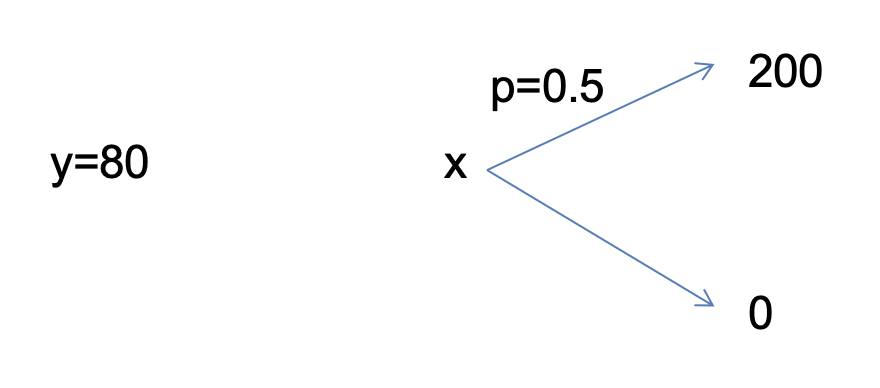
\includegraphics[width=0.5\textwidth]{L1UT1}
    \centering
\end{figure}
\end{frame}

\begin{frame}
Axioms of Rational Behaviour\\
\hfill \break
2. \textit{Transitivity}: the preference ordering is transitive\\
\begin{center}
    if $x \succ y$ and $y \succ z \implies x \succ z$\\
    if $x \sim y$ and $y \sim z \implies x \sim z$
\end{center}
\begin{figure}[ut2]
    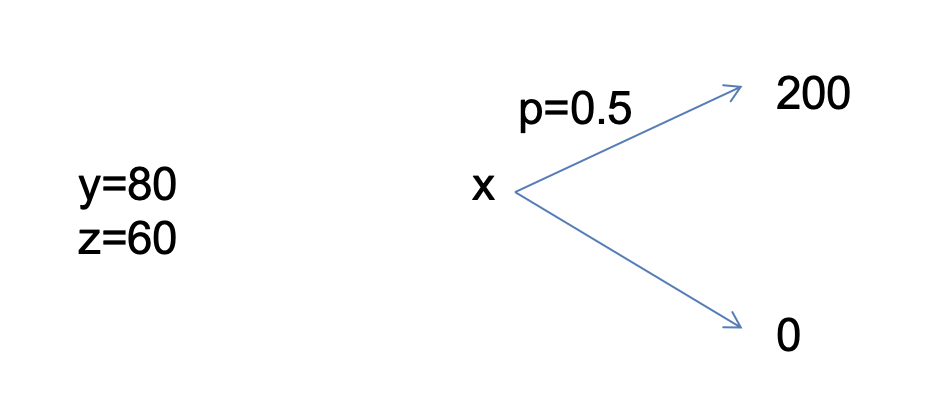
\includegraphics[width=0.5\textwidth]{L1UT2}
    \centering
\end{figure}
\end{frame}

\begin{frame}
Axioms of Rational Behaviour\\
\hfill \break
3. \textit{Independence}: Let $g(x,z;p)$ represent a gamble with probability p of paying x and (1-p) of paying z\\
\begin{figure}[ut3]
    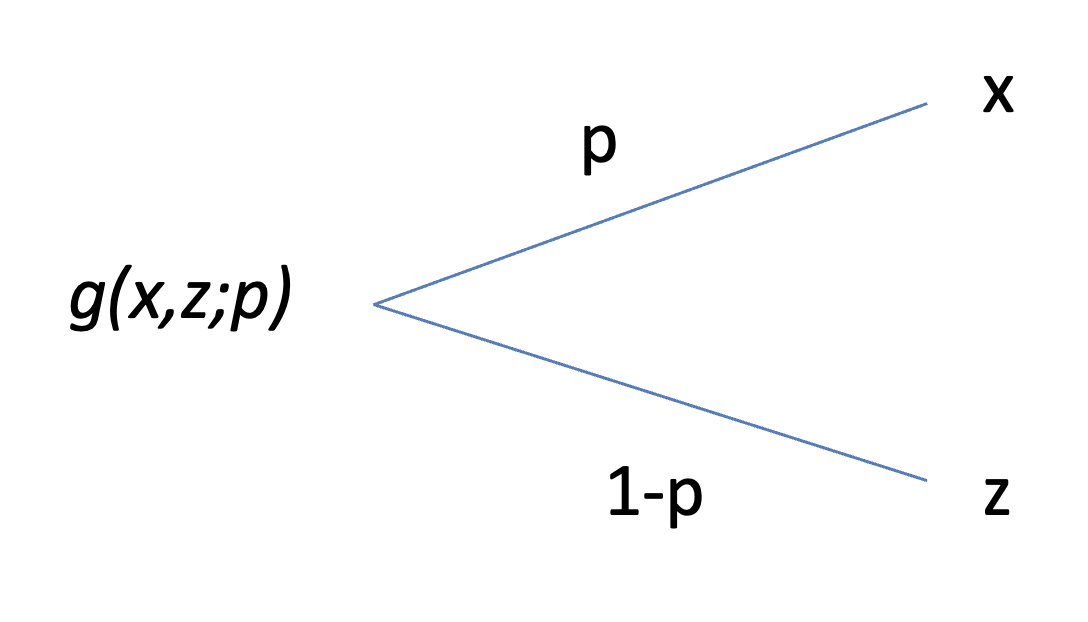
\includegraphics[width=0.4\textwidth]{L1UT3}
    \centering
\end{figure}
\begin{align*}
    &\textrm{if } x \sim y\\
    &\textrm{then } g(x,z;p) \sim g(y,z;p)
\end{align*}
\end{frame}

\begin{frame}
Axioms of Rational Behaviour\\
\hfill \break
4. \textit{Continuity}: If $x \succsim y \succsim z$ then there exists a probability p (unique unless $x \sim y \sim z$) such that $y \sim g(x,z;p)$\\
\begin{figure}[ut4]
    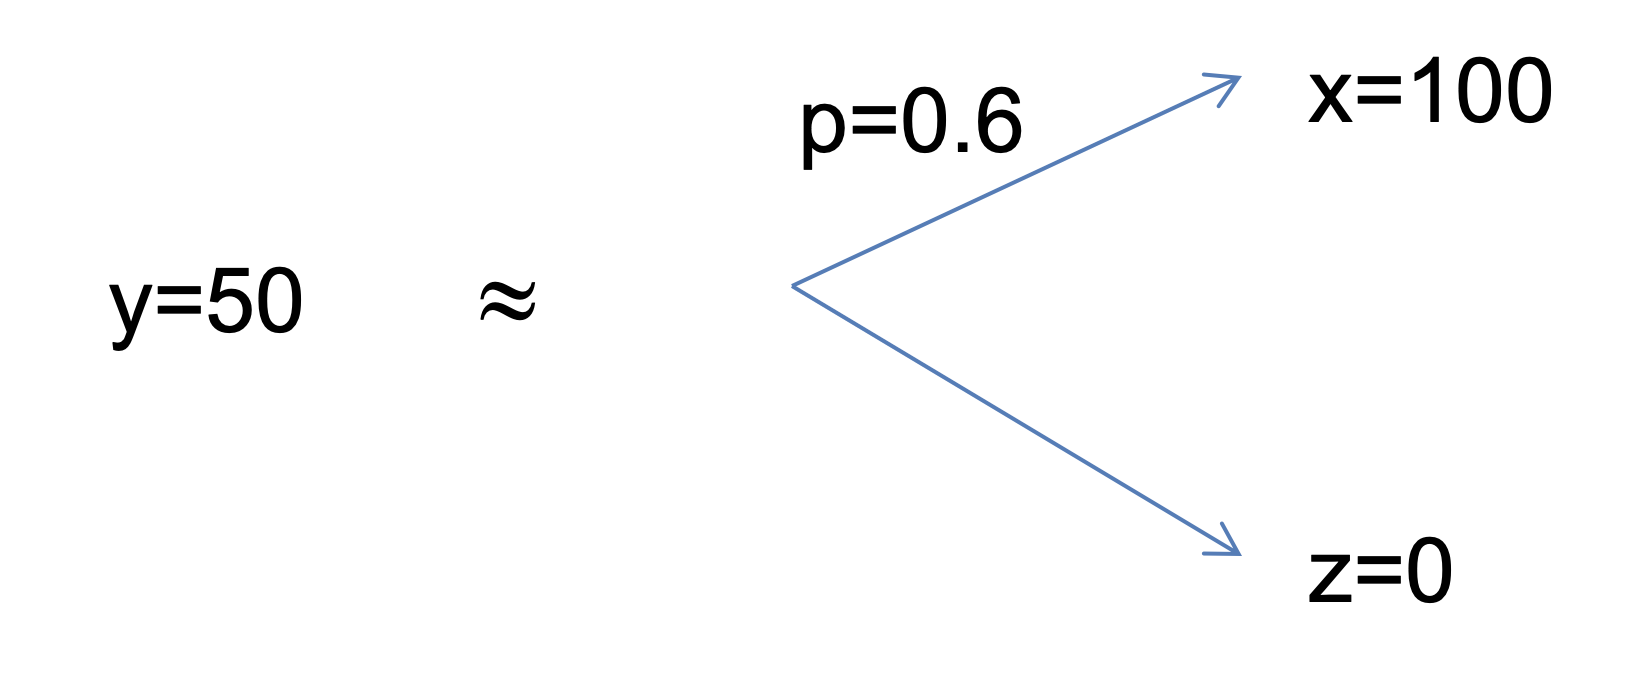
\includegraphics[width=0.5\textwidth]{L1UT4}
    \centering
\end{figure}
\end{frame}

\begin{frame}
Axioms of Rational Behaviour\\
\hfill \break
5. \textit{Dominance}: If $x \succ y \succ z$ and $x \succ t \succ z$, $y \sim g(x,z;p_1)$ and $t \sim g(x,z;p_2)$\\
\begin{center}
    then $p_1 > p_2 \implies y \succ t$\\
    and $p_1 = p_2 \implies y \sim t$\\
\end{center}
\begin{figure}[ut5]
    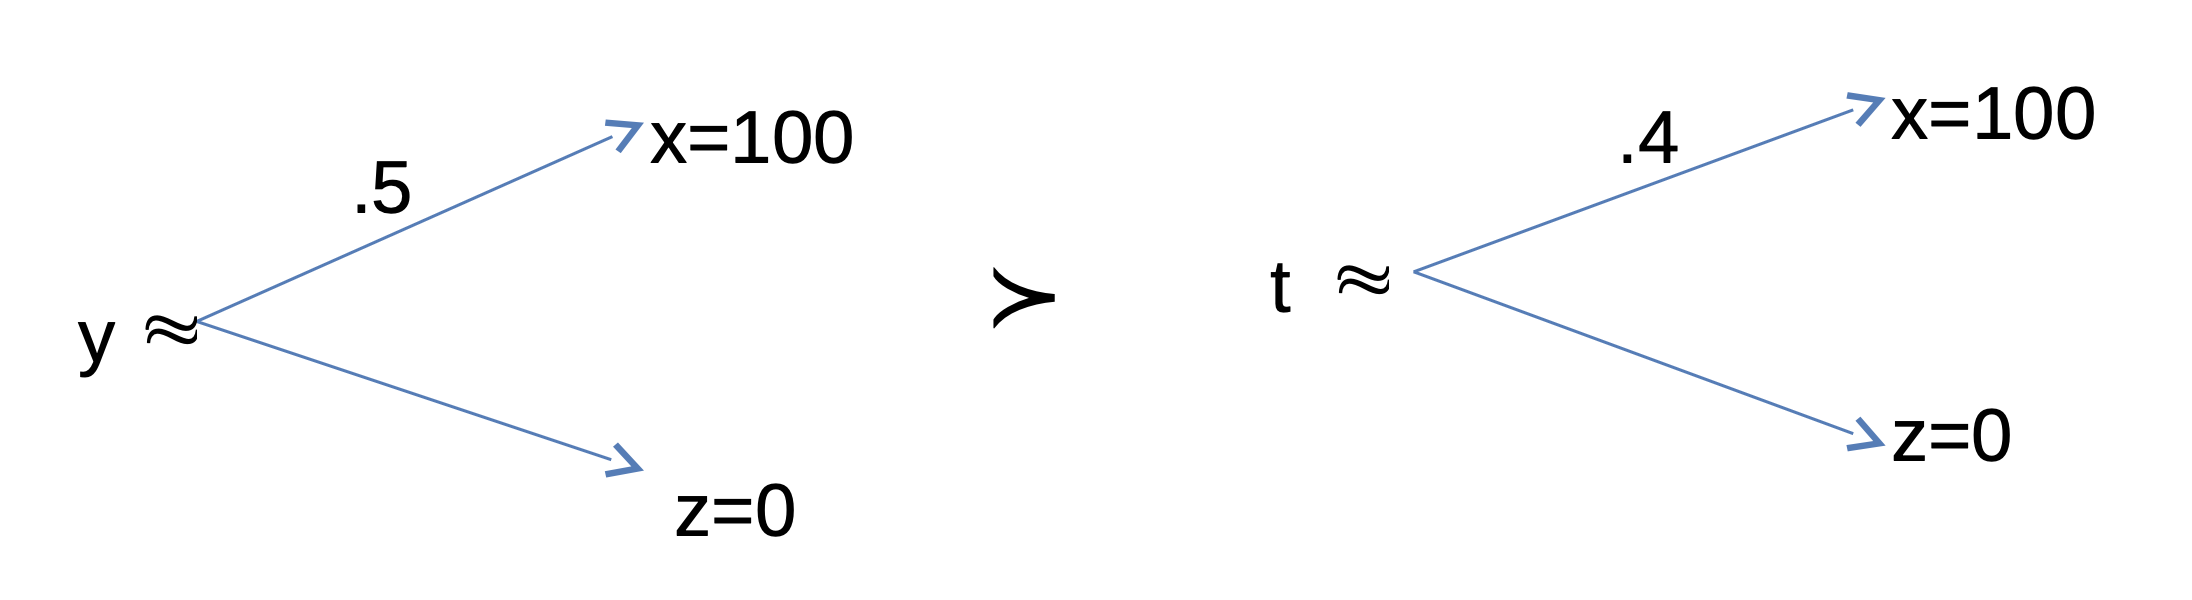
\includegraphics[width=0.6\textwidth]{L1UT5}
    \centering
\end{figure}
\end{frame}

\begin{frame}
Rational Preferences Under Uncertainty\\
\hfill \break
\textbf{Existence}: A preference ordering on risky prospects which satisfy these rationality requirements can be represented by a utility function u defined over the set of outcomes in the sense that\\
\hfill \break
\begin{center}
    $E[u(x)] \geq E[u(y)]$\\
    $iff\;x \succsim y$\\
\end{center}
\end{frame}

\begin{frame}
Rational Preferences Under Uncertainty\\
\hfill \break
\textbf{Uniqueness}: u(x) is unique up to a positive linear transformation.\\
\hfill \break
If u(x) is a utility function, so is $v(x)=au(x)+b$ with $a>0$ \\
\begin{center}
    $E[v(x)] \geq E[u(y)]$\\
    $E[au(x)+b] \geq E[au(y)+b]$\\
    $aE[u(x)]+b \geq aE[u(y)]+b$\\
    $E[u(x)] \geq E[u(y)]$\\
\end{center}
\end{frame}


\subsection{Risk Aversion}

\begin{frame}
Concave utility function for wealth: $u''<0$\\
\begin{figure}[l1-concave]
    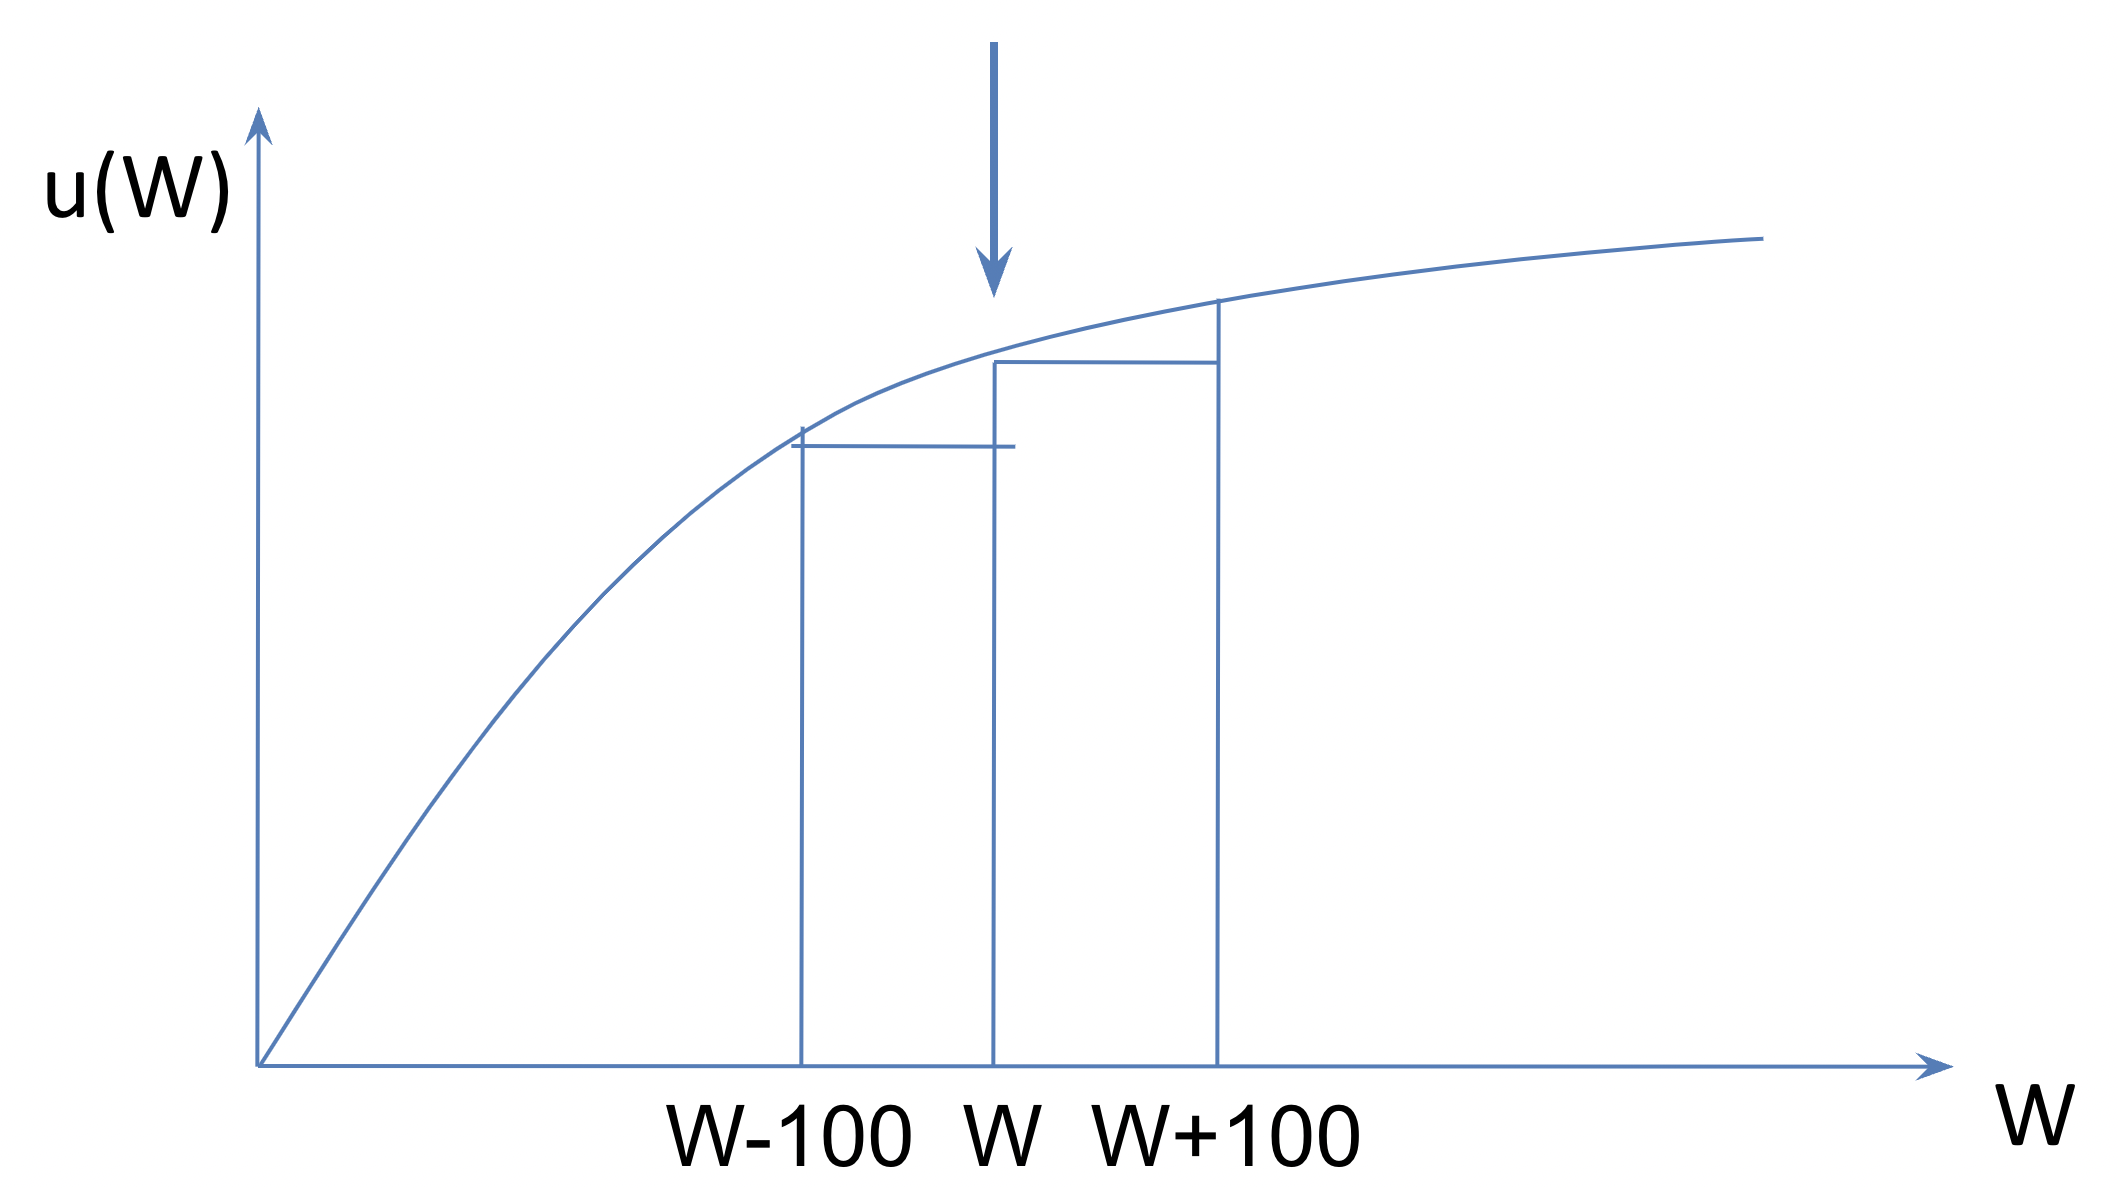
\includegraphics[width=0.5\textwidth]{L1-concave}
    \centering
\end{figure}
\hfill \break
Feel more “pain” to lose \$100 than “pleasure” to win \$100. Decreasing marginal utility of money\\
\hfill \break
($u'>0$ since more is preferred to less!)\\
\end{frame}

\begin{frame}
Risk Averse\\
\hfill \break
\begin{itemize}
    \item Investor will not trade \$100 for sure for 50/50 chance of getting \$200 or nothing
    \item With concave utility:
\end{itemize}
\[ u(100) > 0.5 u(200) + 0.5 u(0)\]
\begin{figure}[l1-ra]
    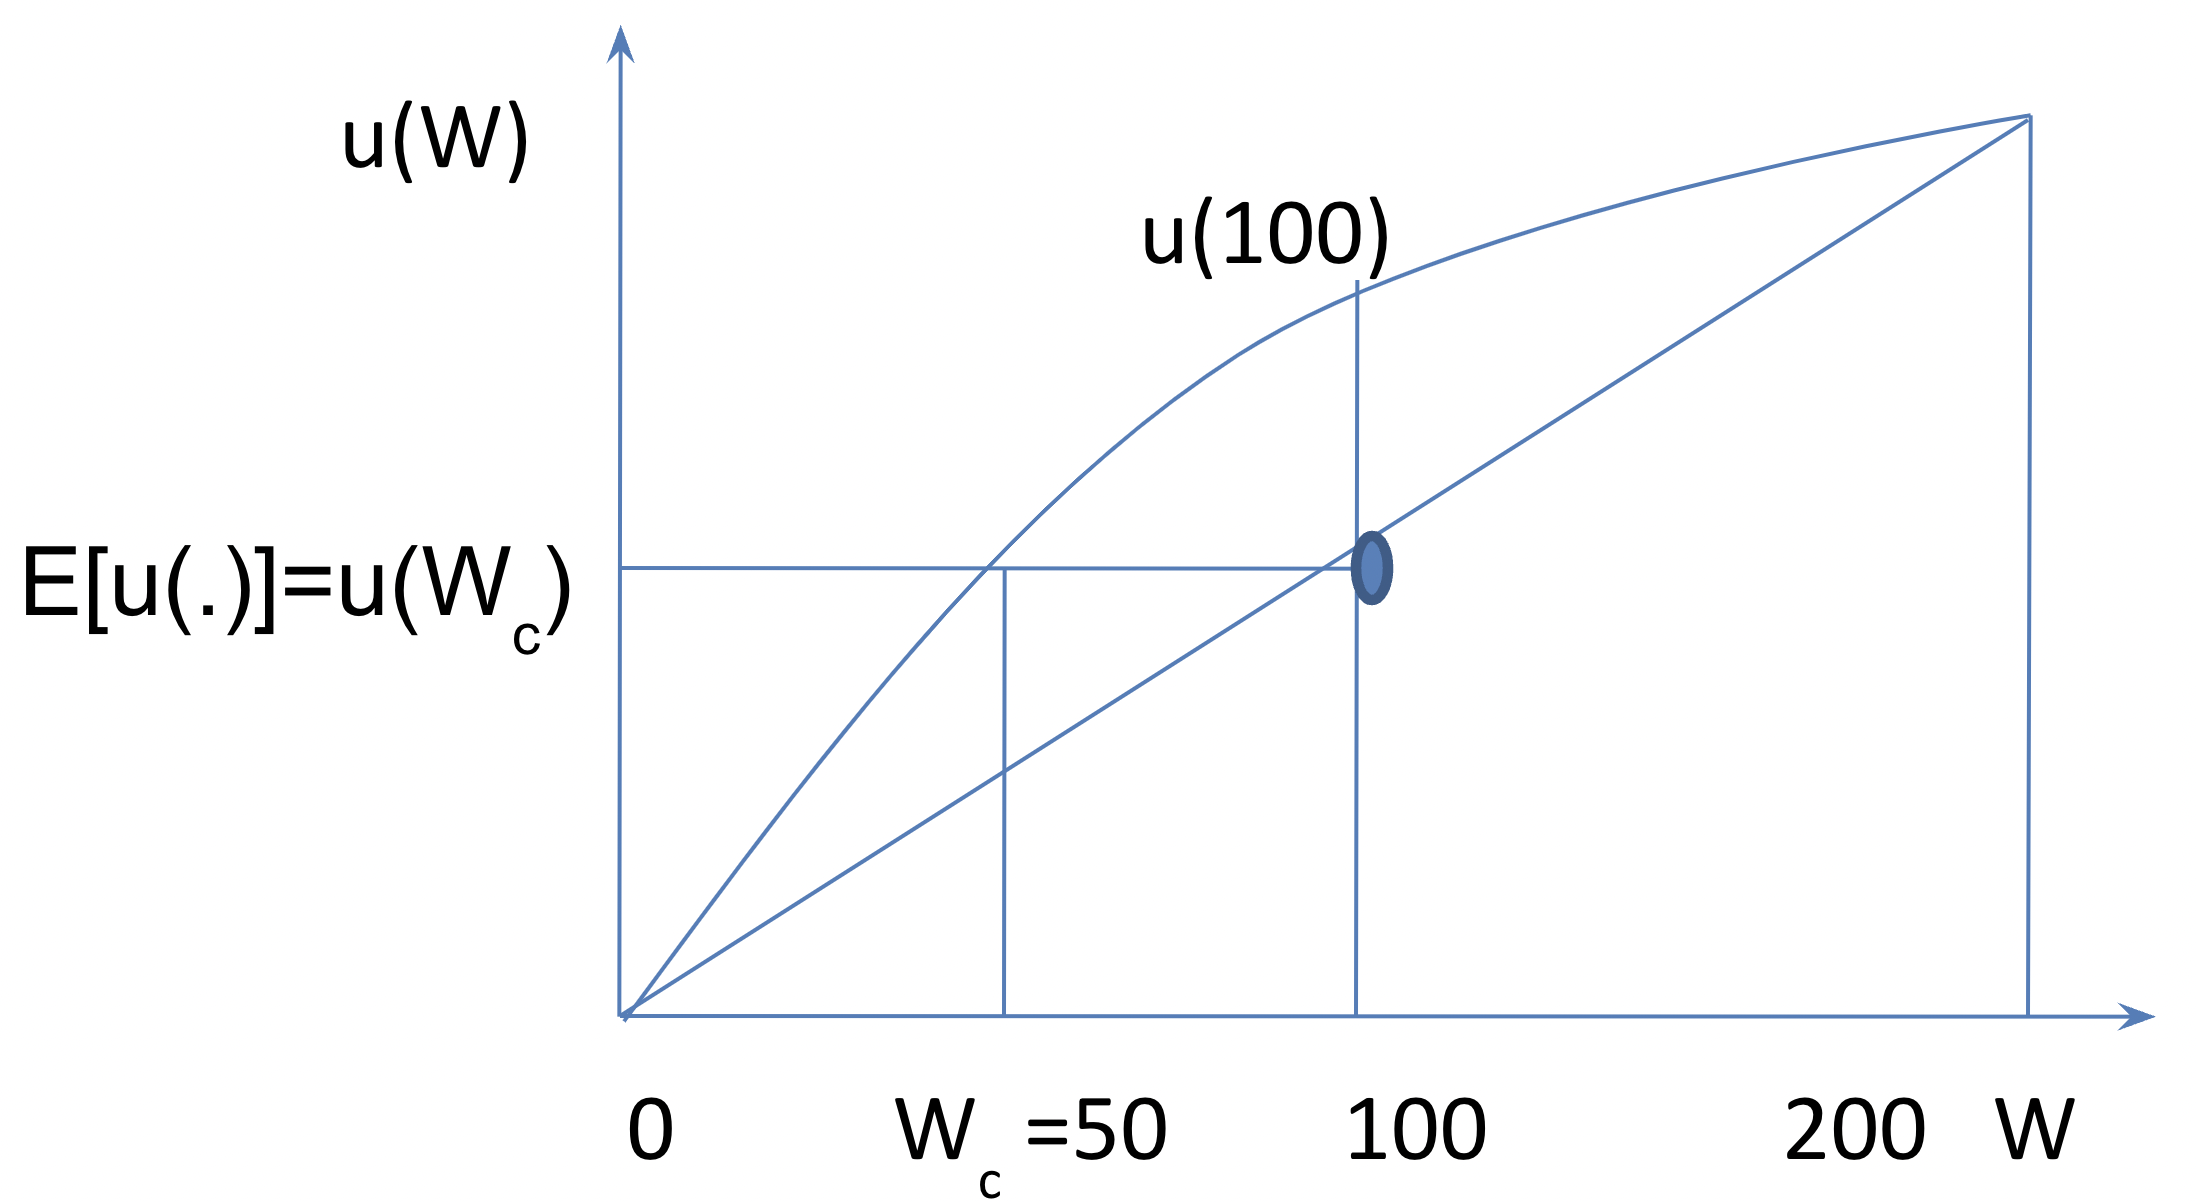
\includegraphics[width=0.5\textwidth]{L1-riskaversion}
    \centering
\end{figure}
\end{frame}

\begin{frame}
Risk Neutral\\
\hfill \break
\begin{itemize}
    \item Linear utility function for wealth: $u''=0$
\end{itemize}
\begin{figure}[l1-rn]
    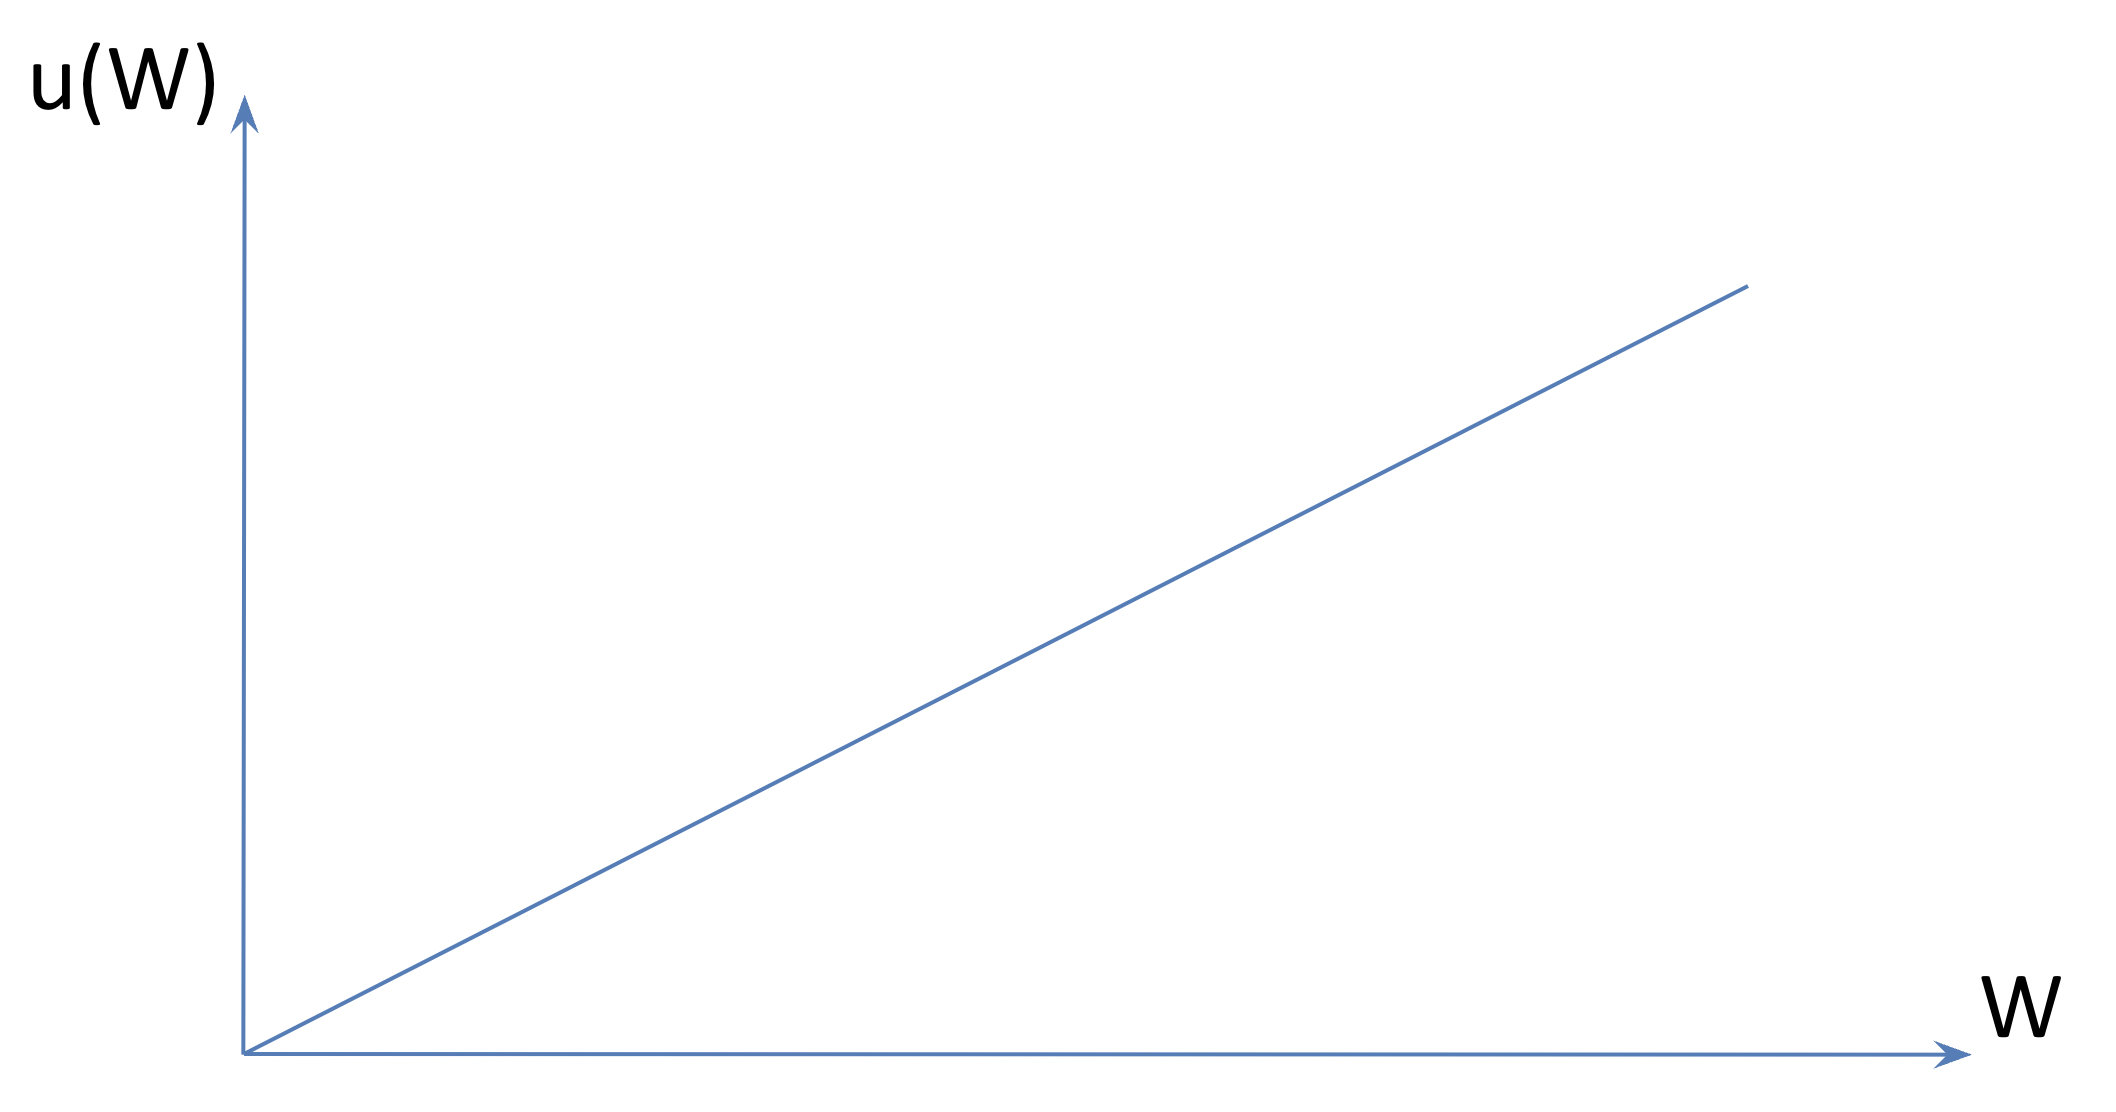
\includegraphics[width=0.6\textwidth]{L1-riskneutral}
    \centering
\end{figure}
Investor maximizes expected wealth\\
\end{frame}

\begin{frame}
Risk Seeking\\
\hfill \break
\begin{itemize}
    \item Convex utility function for wealth: $u''>0$
\end{itemize}
\begin{figure}[l1-rs]
    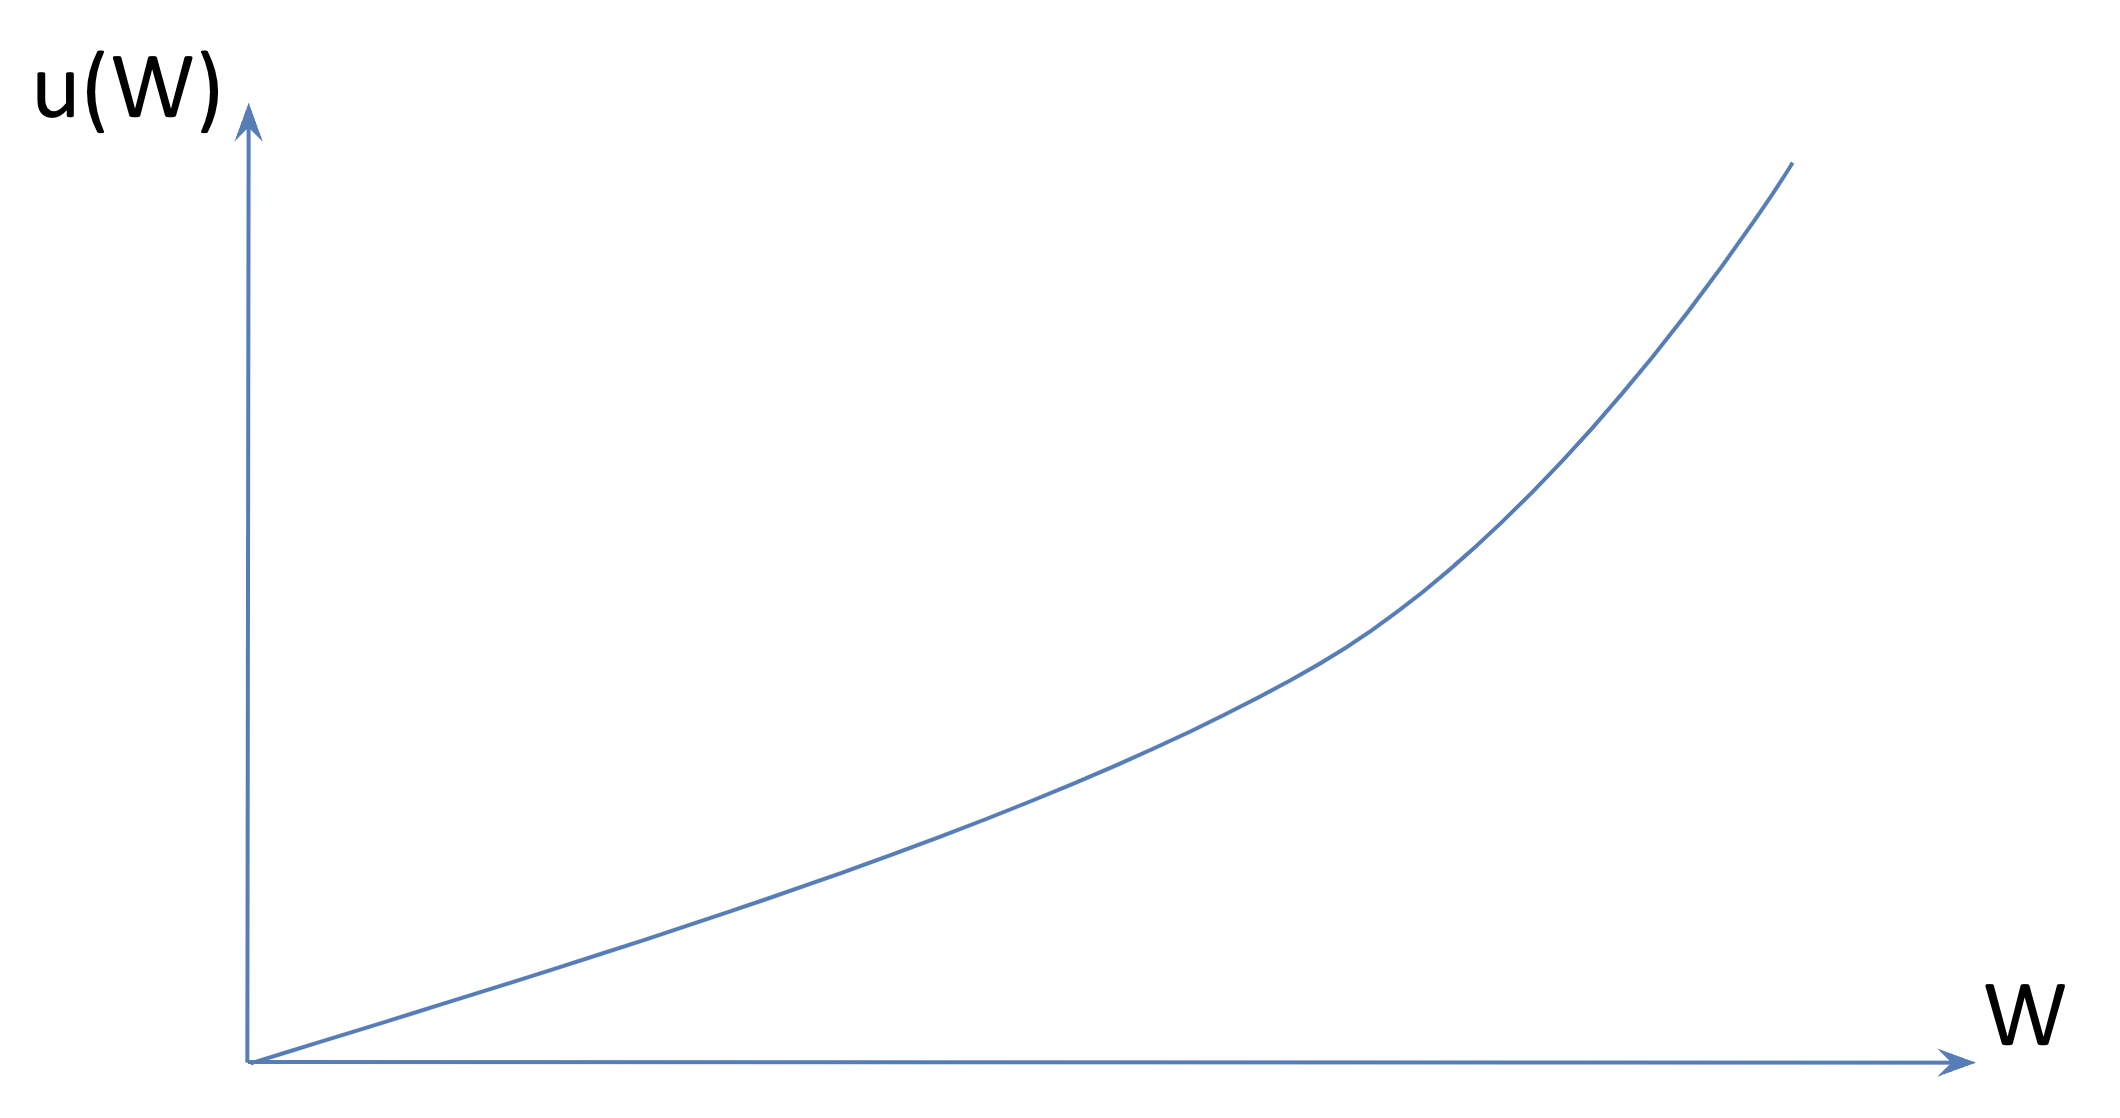
\includegraphics[width=0.6\textwidth]{L1-riskseeker}
    \centering
\end{figure}
Gambling?\\
\end{frame}

\begin{frame}
\textbf{Certainty Equivalent for Complex Gambles ($W_c$)}\\
\begin{center}
    $u(W_c) > E[u(complex\;gamble)]$\\
\end{center}
\begin{center}
    Amount you would accept for certain instead of the gamble.
\end{center}
\hfill \break
If $\bar{W}$ is the expected outcome:\\
\begin{enumerate}
\setlength{\itemindent}{.5in}
    \item risk averse if $W_c < \bar{W} \impliedby u''<0$  concave
    \item risk neutral if $W_c = \bar{W} \impliedby u''=0$  linear
    \item risk seeker if $W_c > \bar{W} \impliedby u''>0$  convex
\end{enumerate}
\end{frame}

\begin{frame}
Risk Averse Certainty Equivalent\\
\begin{figure}[l1-ce]
    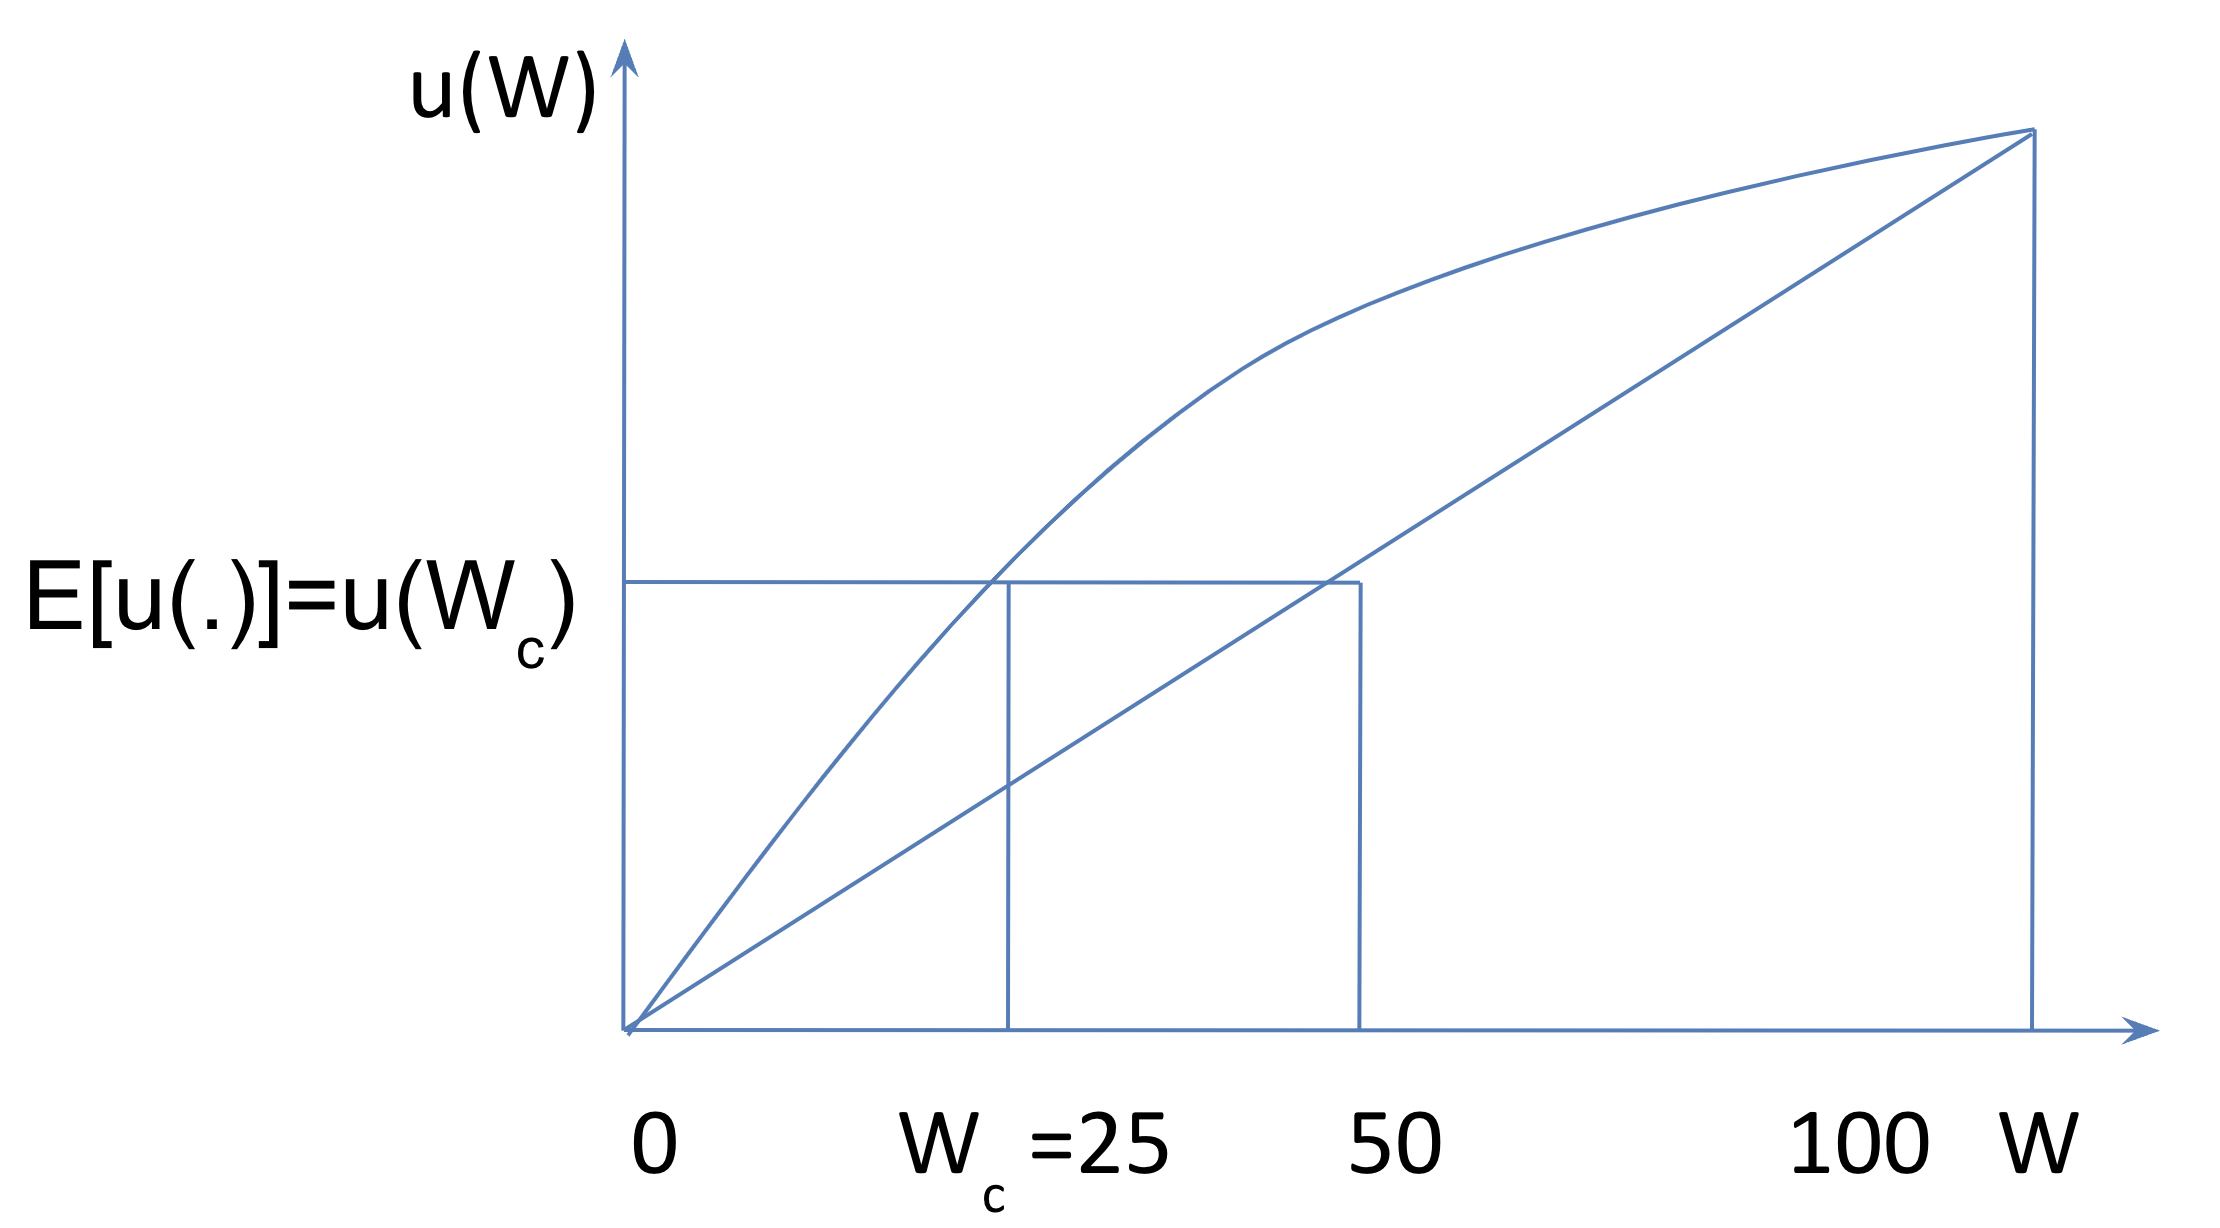
\includegraphics[width=0.5\textwidth]{L1-certaintyequiv}
    \centering
\end{figure}
\begin{figure}[l1-ce2]
    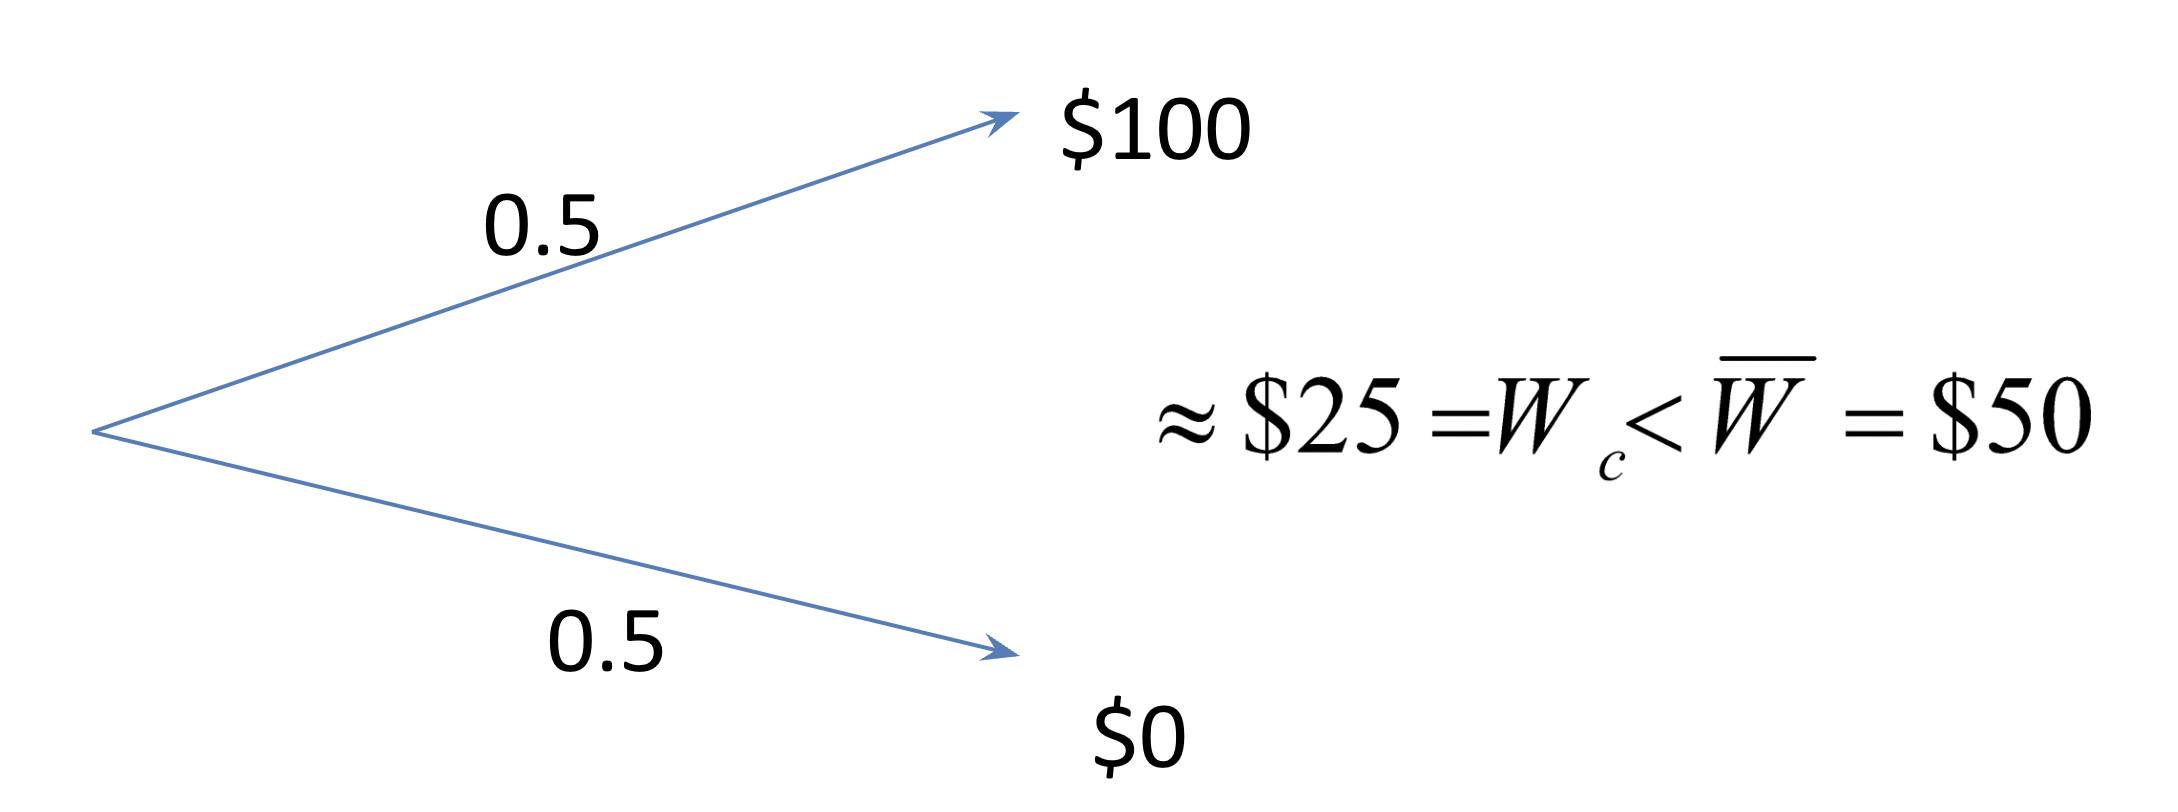
\includegraphics[width=0.5\textwidth]{L1-certaintyequiv2}
    \centering
\end{figure}
\end{frame}

\subsection{Absolute and Relative Risk Aversion}

\begin{frame}
\textbf{Measures of Risk Aversion}\\
\hfill \break
Size of  $u''(W)<0$  is not meaningful (unique up to a positive linear transformation),  $u'(W)>0$ more is preferred to less.\\
\begin{itemize}
    \item Absolute Risk Aversion $\;A(W) = -\frac{u''(W)}{u'(W)}$\\
    \item Relative Risk Aversion $\;\;R(W) = -\frac{Wu''(W)}{u'(W)} = W\cdot A(W)$\\
\end{itemize}
\hfill \break
Independent of positive linear transformation of the utility fn.
\begin{center}
    $v(W)=au(W)+b$, with $a>0$\\
\end{center}
Allows comparisons between individuals.\\
\end{frame}

\begin{frame}
\textbf{Measures of Risk Aversion}\\
\hfill \break
\begin{align*}
    v(W)&=au(W)+b, a>0\\
    v'(W)&=au'(W)>0\\
    v''(W)&=au''(W)<0\\
\end{align*}
\begin{align*}
    A(W)&=-\frac{u''(W)}{u'(W)}=-\frac{v''(W)}{v'(W)}>0\\
    R(W)&=-\frac{Wu''(W)}{u'(W)}=-\frac{Wv''(W)}{v'(W)}>0\\
\end{align*}
\end{frame}

\subsection{Useful Utility Functions}
\begin{frame}
\textbf{Exponential}: constant absolute risk aversion\\
\begin{align*}
    u(W)&=-\frac{1}{a}e^{-aW} \textit{ with } a>0\\
    u'(W)&=e^{-aW}>0\\
    u''(W)&=-ae^{-aW}<0\\
    A(W)&=-\frac{u''(W)}{u'(W)} = a
\end{align*}
\begin{figure}[exponential]
    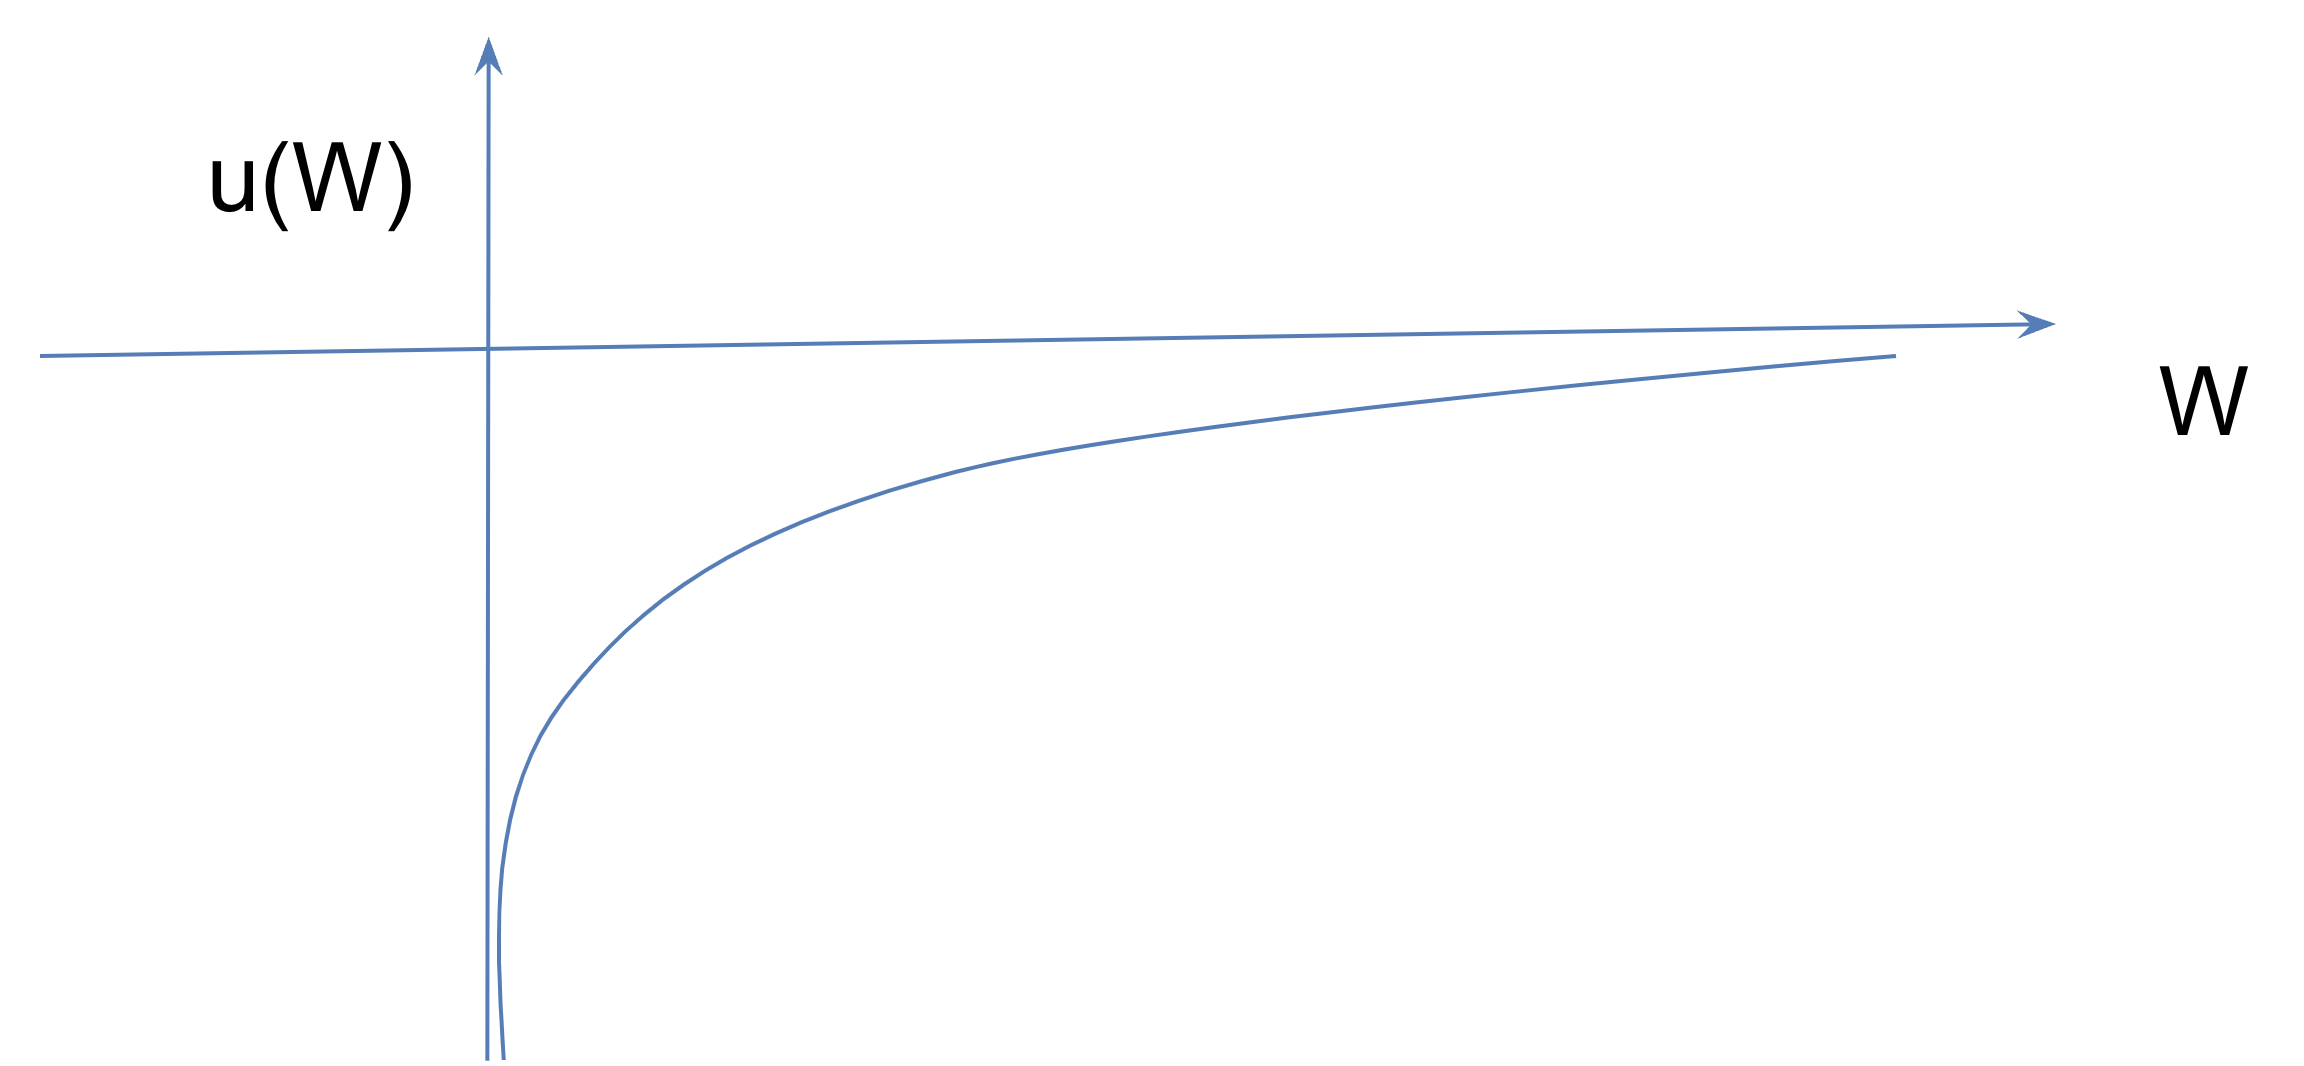
\includegraphics[width=0.4\textwidth]{L1-exp}
    \centering
\end{figure}
\end{frame}

\begin{frame}
\textbf{Power}: constant relative risk aversion\\
\begin{align*}
    u(W)&=\frac{W^\gamma}{\gamma} \textit{ for } \gamma<1, \gamma\neq0\\
    u'(W)&=W^{\gamma-1}>0\\
    u''(W)&=(\gamma-1)W^{\gamma-2}<0\\
    R(W)&=-\frac{Wu''(W)}{u'(W)} = 1-\gamma = c > 0, \gamma < 1 \;\; u(W)=\frac{W^{1-c}}{1-c}
\end{align*}
\begin{figure}[power]
    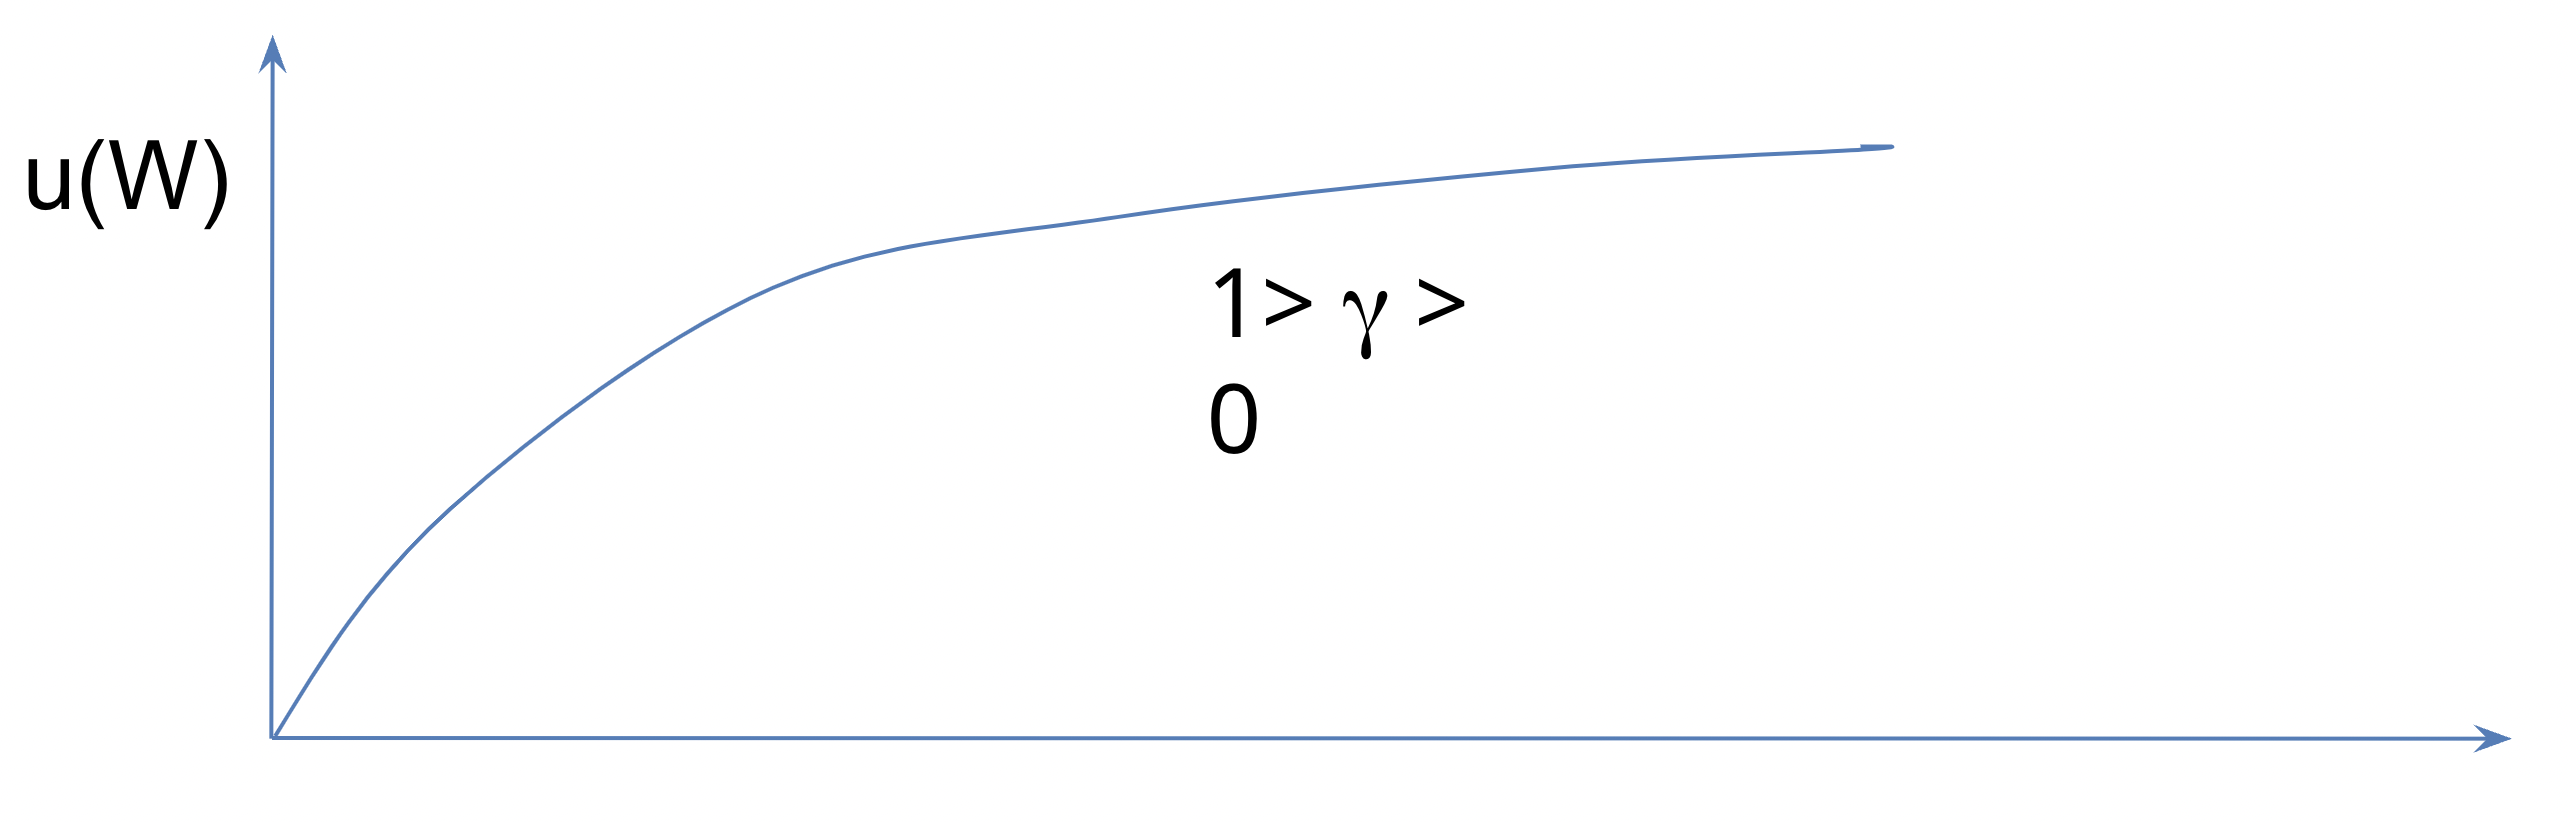
\includegraphics[width=0.5\textwidth]{L1-power}
    \centering
\end{figure}
\end{frame}

\begin{frame}
\textbf{Log}: also constant relative risk aversion\\
\begin{align*}
    u(W)&=\ln{W} (\gamma=0)\\
    u'(W)&=\frac{1}{W}>0\\
    u''(W)&=-\frac{1}{W^2}<0\\
    R(W)&=-\frac{Wu''(W)}{u'(W)}=1
\end{align*}
\begin{figure}[logarithmic]
    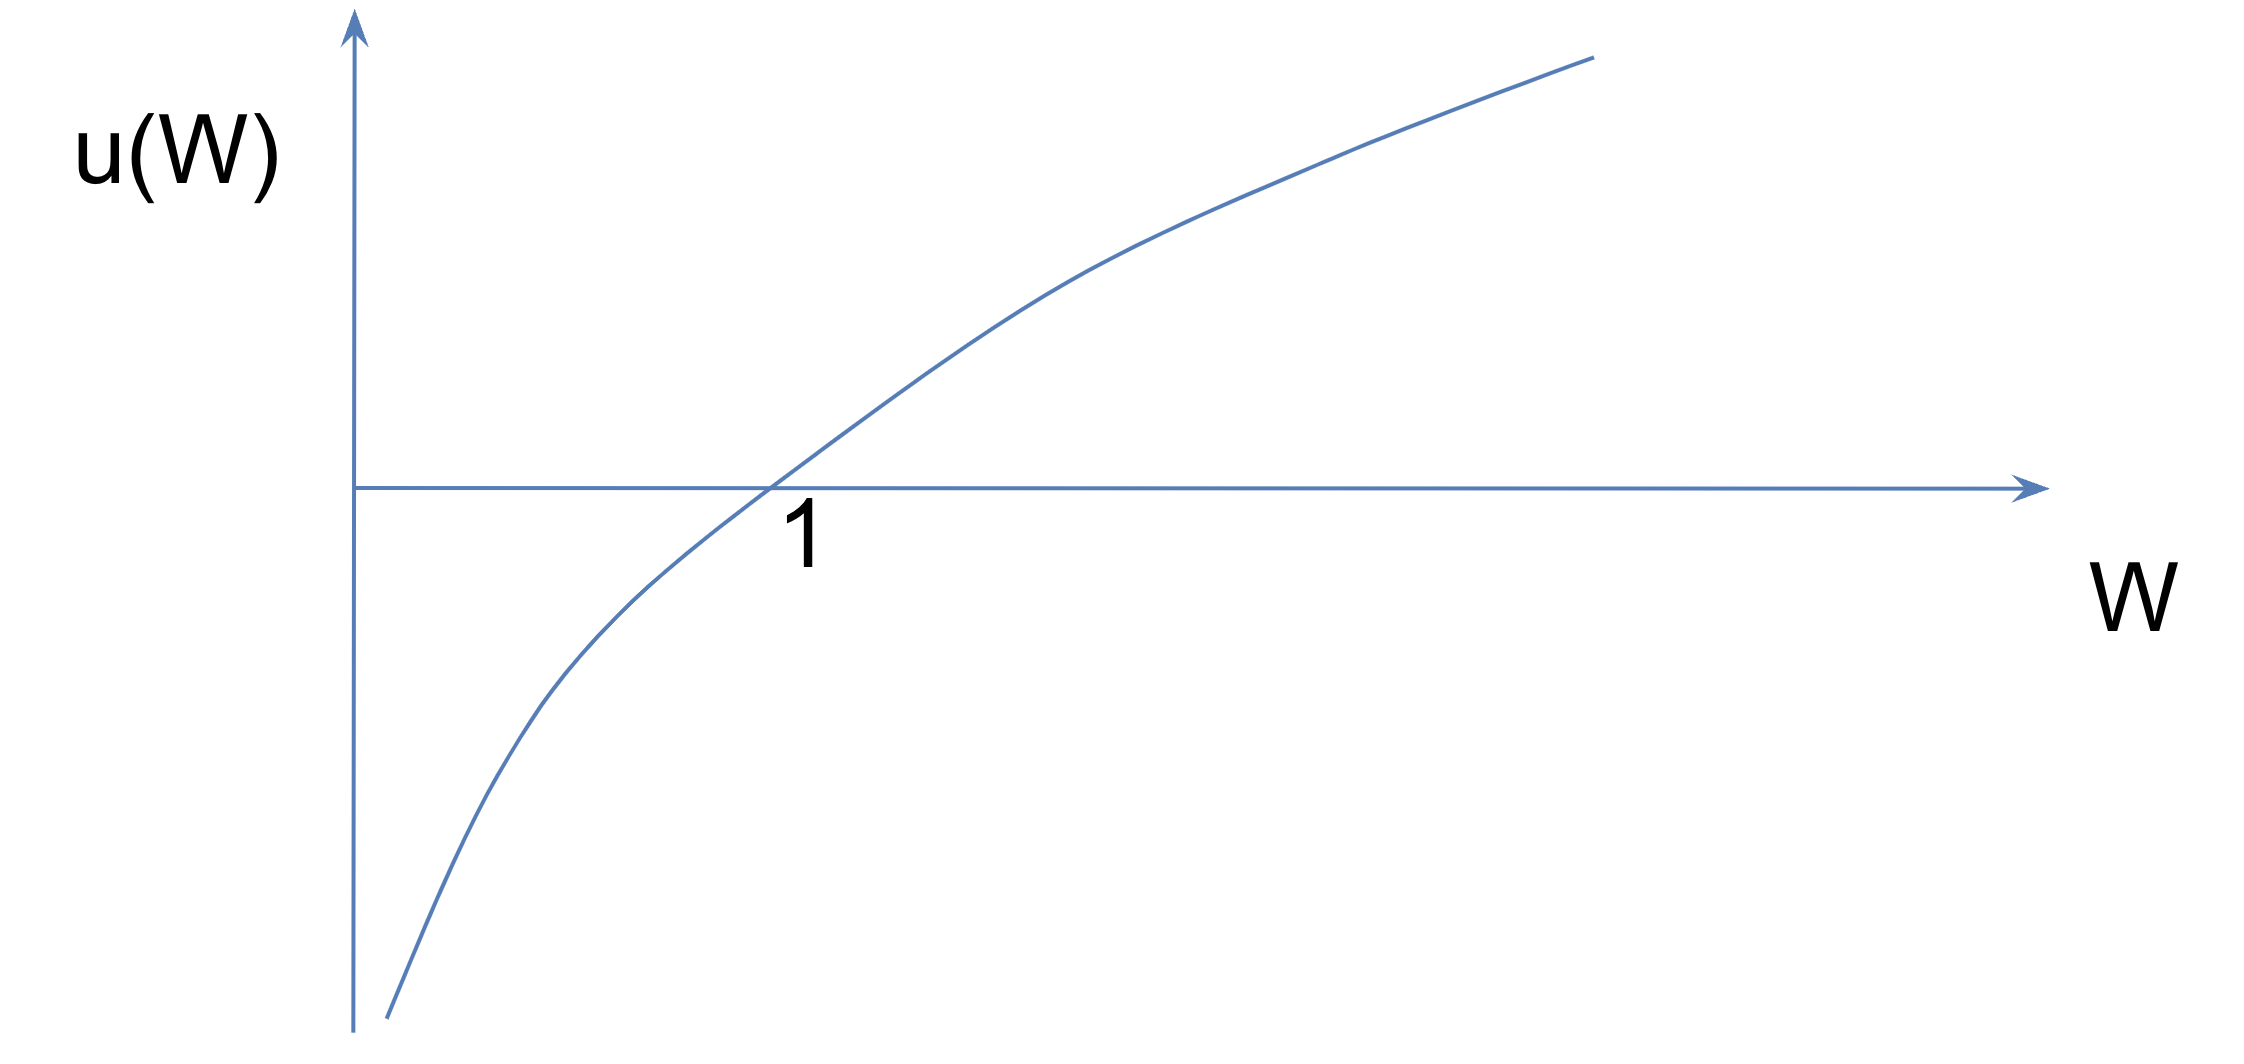
\includegraphics[width=0.4\textwidth]{L1-log}
    \centering
\end{figure}
\end{frame}

\begin{frame}
\textbf{Quadratic}\\
\begin{align*}
    u(W)&=W-\frac{1}{2}bW^2 \textit{\;\;for } 0\leq W\leq \frac{1}{b}\\
    u'(W)&=1-bW>0 \textit{\;\;for } 0\leq W\leq \frac{1}{b}\\
    u''(W)&=-b<0\\
    A(W)&=-\frac{b}{1-bW} \textit{\;\;increasing with W (not good)}
\end{align*}
\begin{figure}[quadratic]
    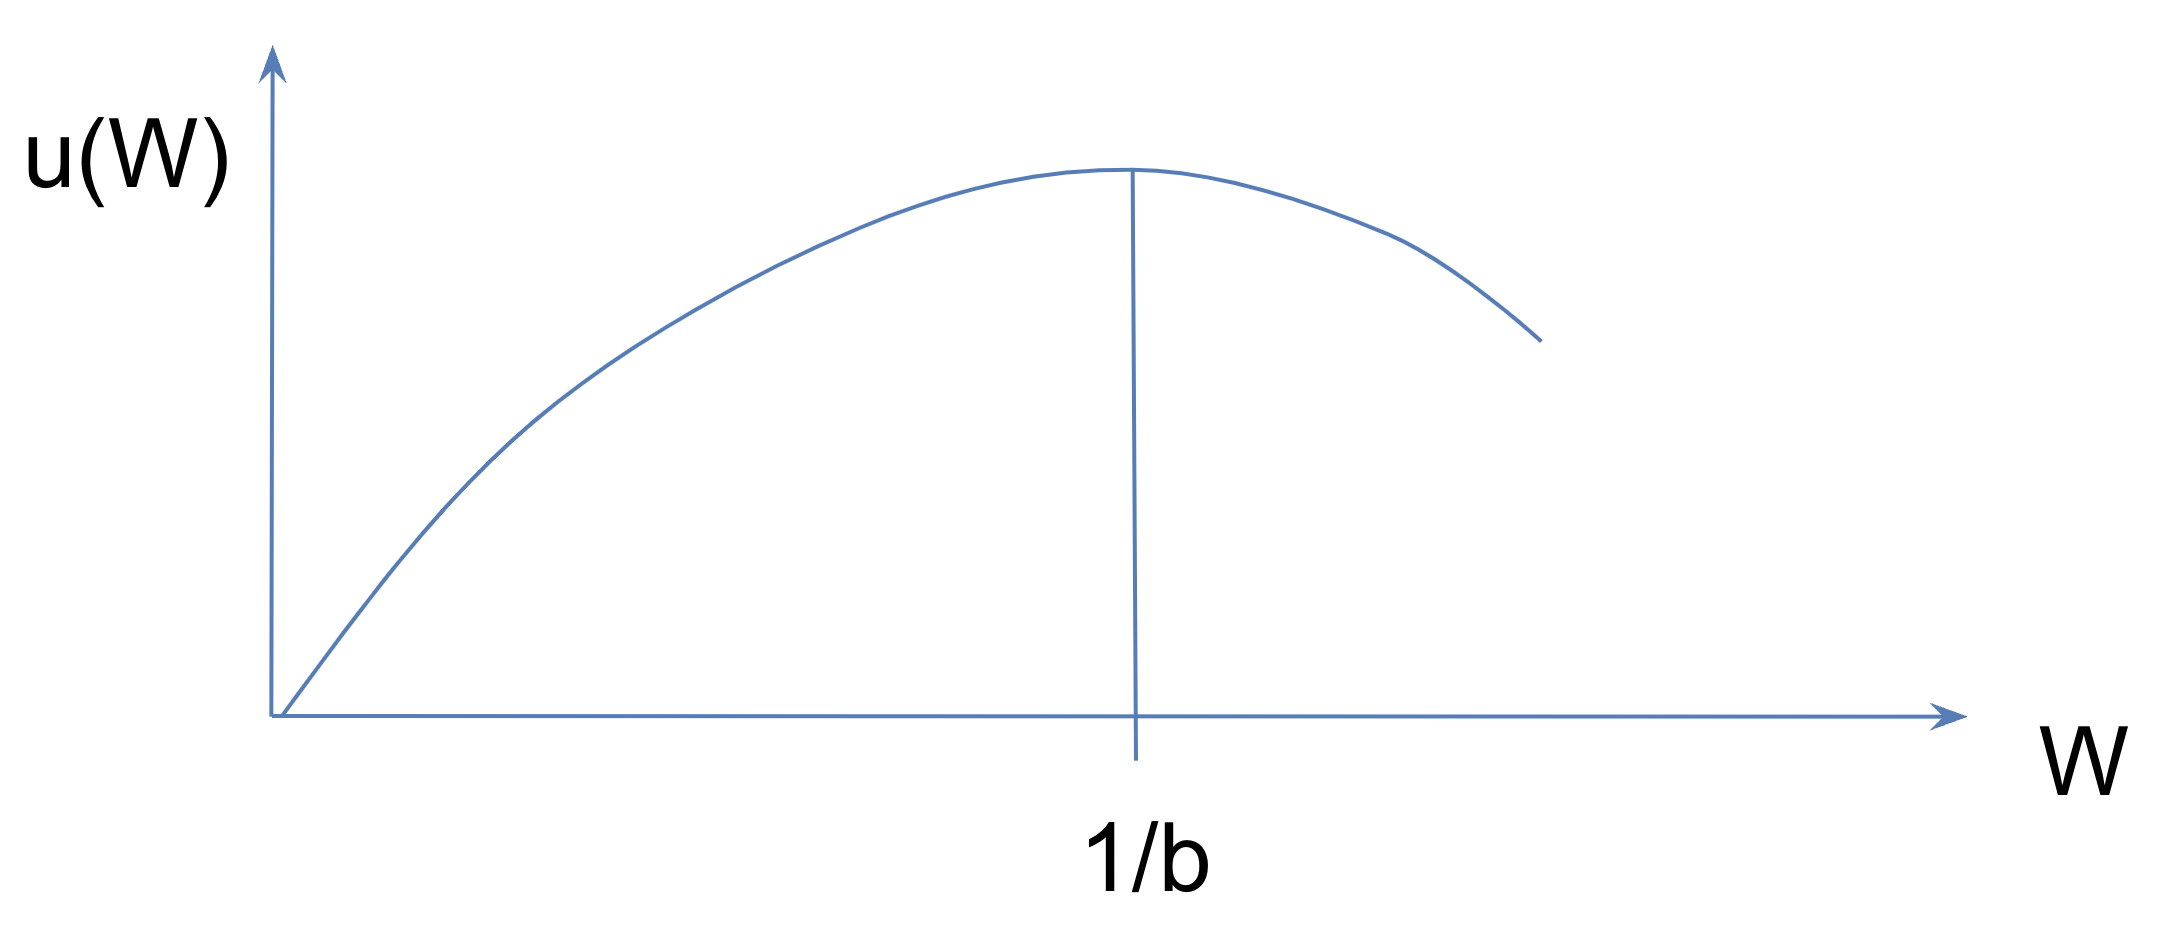
\includegraphics[width=0.4\textwidth]{L1-quad}
    \centering
\end{figure}
\end{frame}

\begin{frame}
Expected utility max. and mean variance analysis are equivalent when...\\
\hfill \break
\begin{outline}
    \1 Utility functions are quadratic
    \begin{align*}
        u(W)&=W-\frac{1}{2}bW^2\\
        E[u(W)]&=\Bar{W}-\frac{1}{2}b[\Bar{W}^2+Var(W)]
    \end{align*}
    \1 Distributions of returns are joint normal
        \2 Normal is completely defined by mean and variance
        \2 Additive
        \2 Indifference curves (constant Eu) can be written in terms of mean and s.d. only
    \1 Be careful when distributions are not normal (options)
\end{outline}
\end{frame}

\begin{frame}
Indifference Curves (for risk averse)\\
\hfill \break
A and B have the same expected utility
\begin{figure}[exponential]
    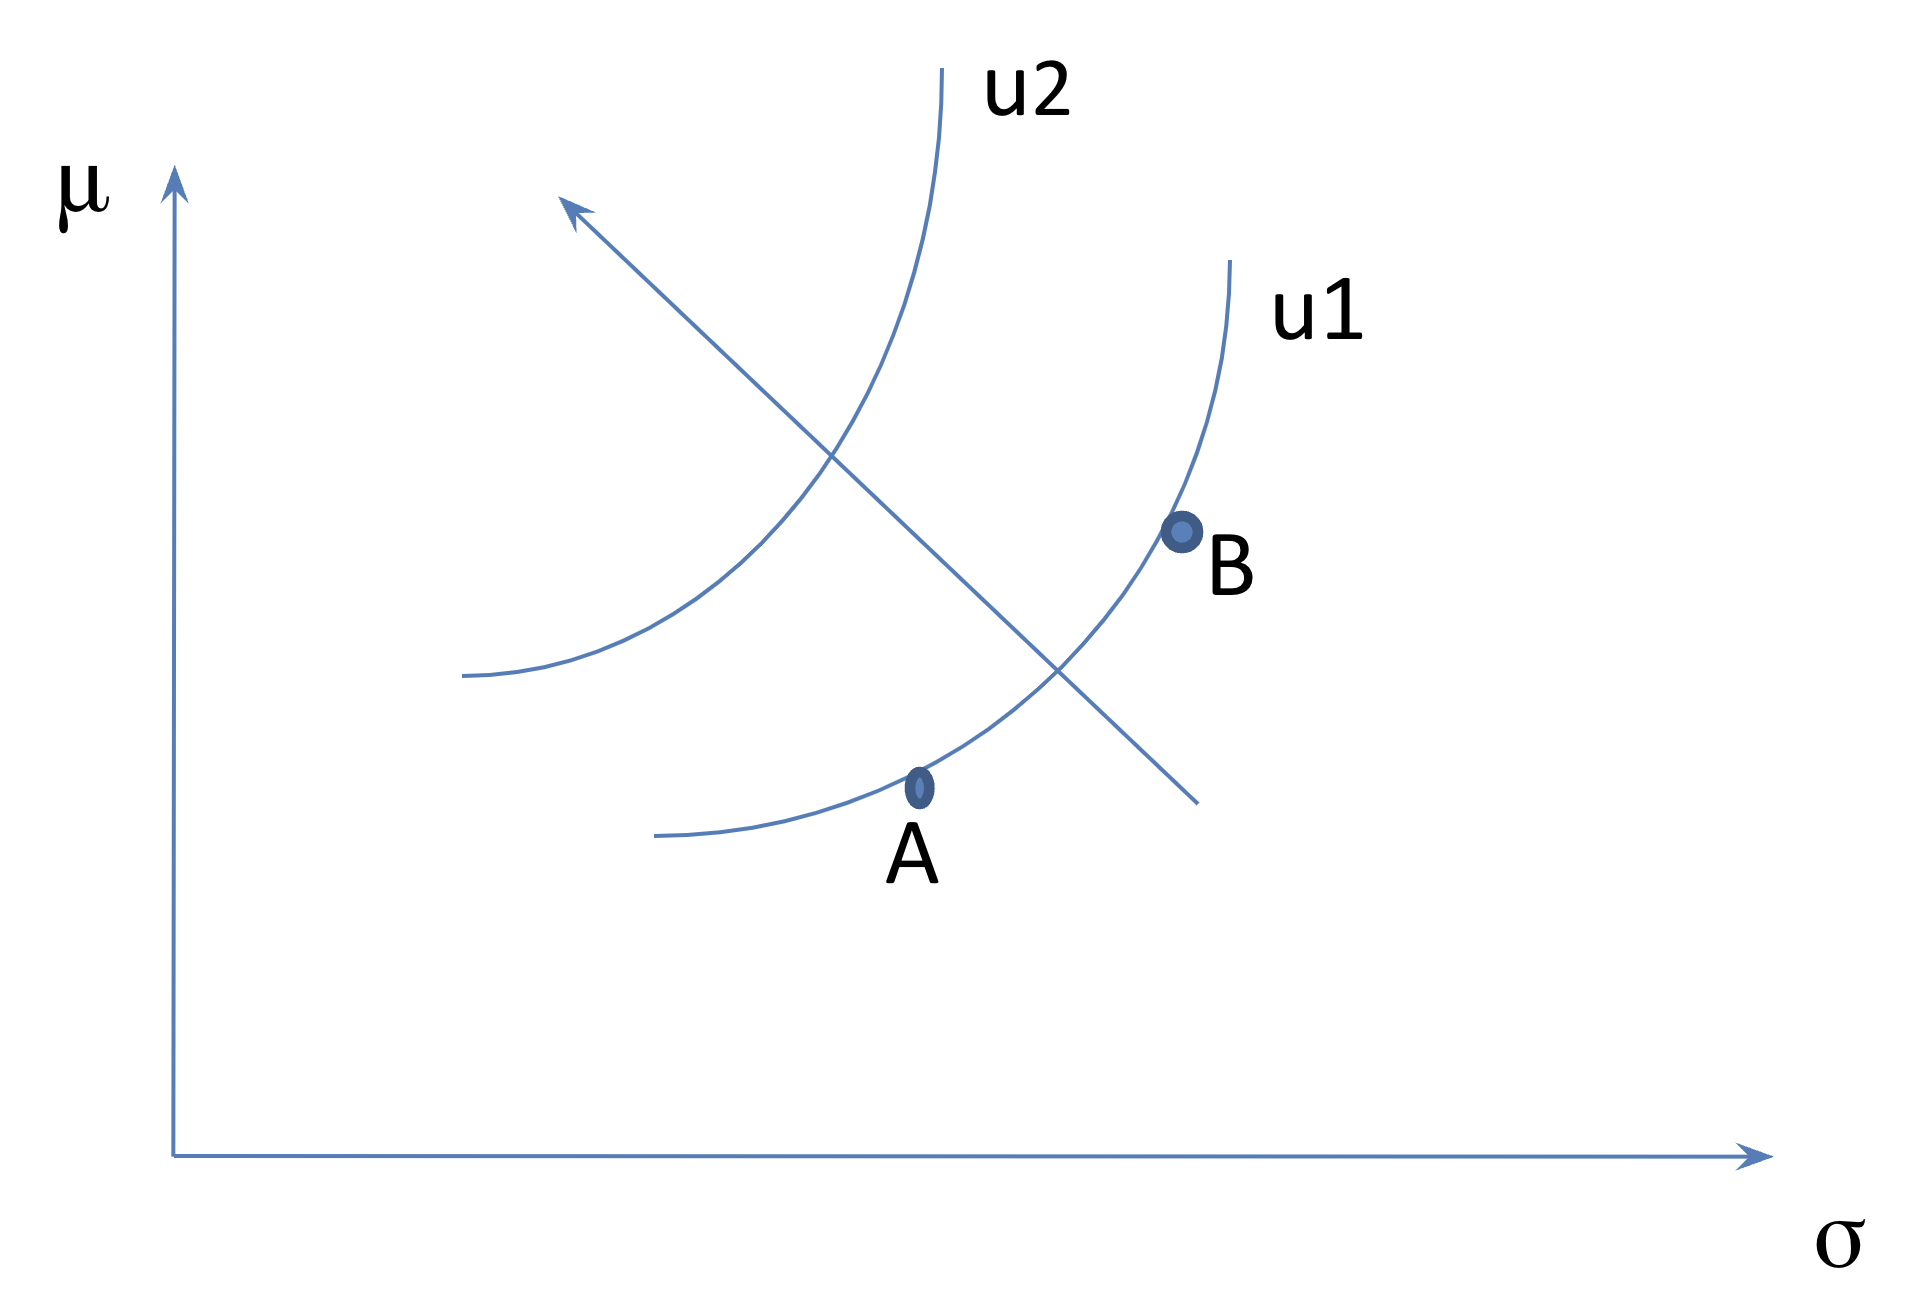
\includegraphics[width=0.6\textwidth]{L1-indiff}
    \centering
\end{figure}
\end{frame}

\begin{frame}
Expected Utility - Example
\hfill \break
\begin{outline}
    \1 Your current wealth is \$100,000.
    \1 You want to purchase a homeowner’s insurance policy to cover potential loss due to fire.
    \1 You estimate that the probability of fire is 10\%
    \1 If your house is damaged by fire your loss would be \$60,000. 
    \1 You have determined that your utility of wealth is $U(W) = \sqrt{W}$. 
    \1 What is the maximum amount you would be willing to pay to fully insure against possible losses due to fire?
\end{outline}
\end{frame}

\begin{frame}
\underline{Expected Utility - Solution}
\hfill \break
\begin{outline}
    \1 Let us assume that you will at the most be willing to pay \$D\break
    \1 If you buy insurance your wealth is \$(100,000 – D) for sure.\break
    \1 If you do not buy insurance there is a 10\% chance that you will end with a wealth of \$40,000 and a 90\% chance that you will end with a wealth of \$100,000\break
\end{outline}
\end{frame}

\begin{frame}
\underline{Expected Utility - Solution}\\
\begin{figure}[ex-util]
    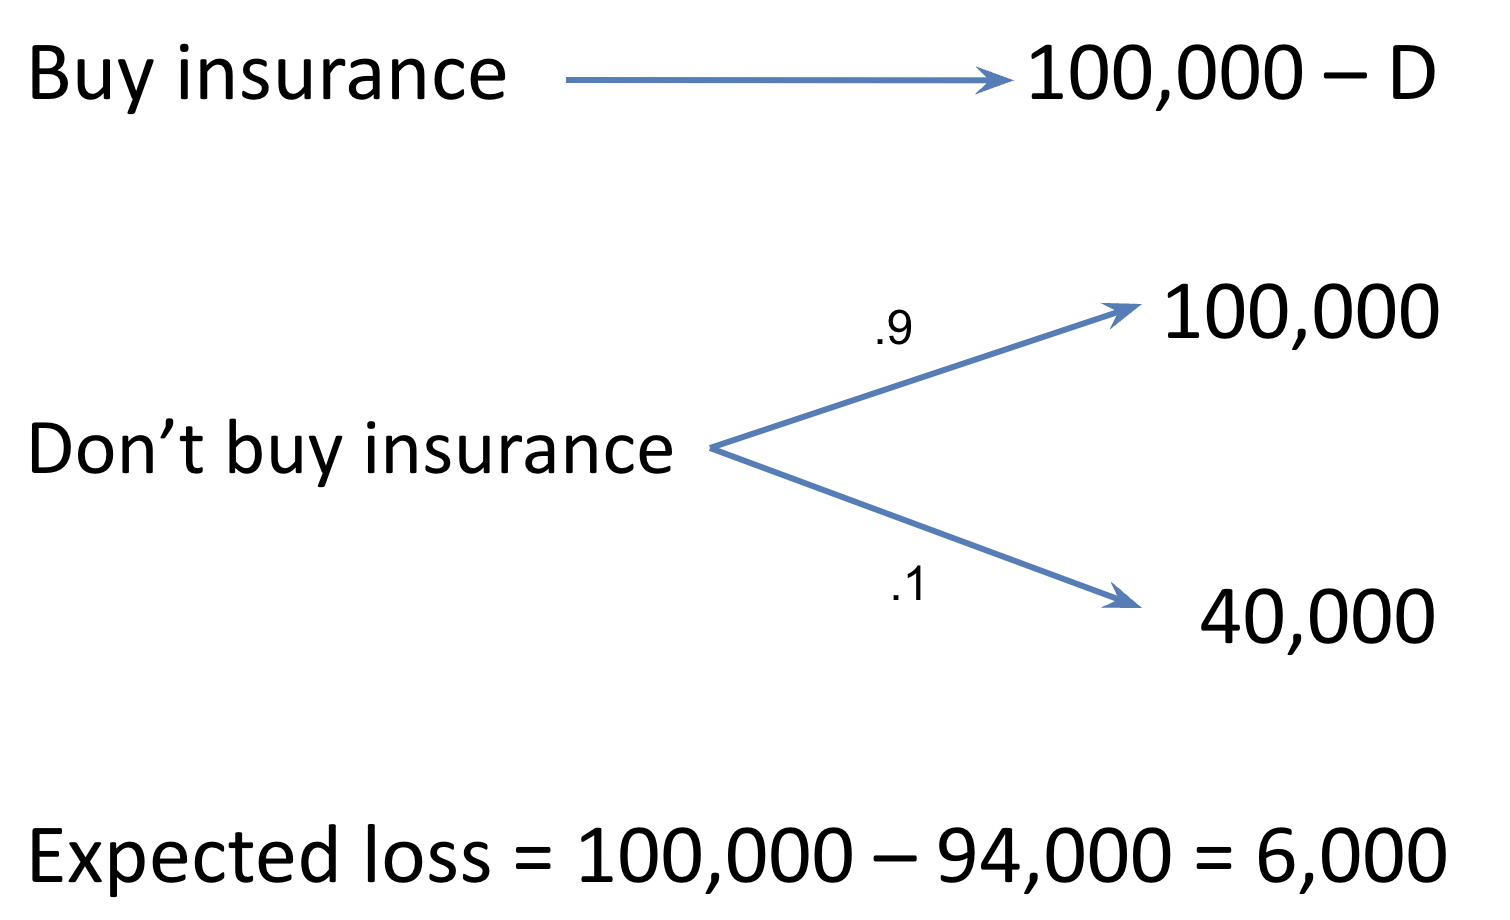
\includegraphics[width=0.7\textwidth]{L1-ex-util}
    \centering
\end{figure}
\end{frame}

\begin{frame}
\underline{Expected Utility - Solution}
\hfill \break
\begin{outline}
    \1 We defined certainty equivalent, $W_c$  as that amount of wealth which makes you indifferent between this wealth and a gamble\break
    \1 That is $U(W_c) = E[U]$
    \begin{align*}
        U(100,000 - D) &= 0.1\cdot U(40,000) + 0.9\cdot U(100,000)\\
        \sqrt(100000-D) &= 0.1\sqrt{40,000} + 0.9\sqrt{100,000}\\
        D &= 7,215.80 > 6,000 \textit{ expected loss }\\
    \end{align*}
\end{outline}
\end{frame}


%%%%%%%%%%%%%%%%%%%%%%%%%%%%%%%%%%%%%%%%%%%%%%%%%%%%%
%%%%%%%%%%%%% TOPIC 2  Utility Theorem %%%%%%%%%%%%%%
%%%%%%%%%%%%%%%%%%%%%%%%%%%%%%%%%%%%%%%%%%%%%%%%%%%%%
\section{Utility Theory}  % TOPIC 2: Utility Theory

\begin{frame}
Rational "preferences" under uncertainty (over consumption hurdles):\\
\begin{outline}
    \1 Completeness
    \1 Transitivity
    \1 Continuity
    \1 Monotonicity (more is preferred to less)
\end{outline}
Ordinal utility fn: any positive transformation preserves the same ordering\\
\end{frame}

\begin{frame}
Rational "preferences" under uncertainty:\\
\hfill \break
Existence and uniqueness theorems based on certain rationality requirements (axioms of rational behaviour).\\
\hfill \break
Even though these axioms have been challenged there is no theory competing with this:\\
\begin{outline}
    \1 measurable or Von Neumann-Morgenstern utility fn.
      \2 "Preferences over gambles"
\end{outline}
\hfill \break
Let $S$ be the set of all risky prospects (or payoff distributions).\\
\end{frame}

\subsection{Expected Utility Theorem}

\begin{frame}
Let $S$ be the set of all risky prospects (or payoff distributions).\\
\hfill \break
\underline{\textbf{Expected Utility Theorem}}:\\
\hfill\break
(Existence) A preference ordering on $S$ which satisfies certain rationality requirements (A1-A5) can be represented by a utility function $u$ defined on the set of outcomes in the sense that:\\
\begin{align*}
    E[u(x)] \geq& E[u(y)]\\
    x, y \; \epsilon& \; S\\
    \textit{ iff } x \succsim & \; y\\
\end{align*}
\end{frame}

\begin{frame}
\underline{\textbf{Expected Utility Theorem}}:\\
\hfill\break
(Uniqueness) If $u(x)$ is a utility function, so is $au(x)+b\textit{, }a>0$. That is, $u(x)$ is unique up to a positive linear transformation. \\
\begin{align*}
    E[u(x)] =& \sum_i u(x)_i p(x_i)\\
    =& \int_{-\infty}^\infty u(x)f(x)dx\\
    =& \int_{-\infty}^\infty u(x)dF(x)\\
    F(x) =& Pr\{X \leq x\}\\
    f(x) =& \frac{dF(x)}{dx}\\
\end{align*}
\end{frame}

\subsection{Axioms}

\begin{frame}
Axioms governing investors' behavior\\
\hfill \break
\textbf{A1 (Completeness)}: There exists a preference ordering over all risky prospects which is complete.\\
\hfill \break
ie. For any two gambles $x,y$
\hfill \break
\begin{align*}
    x &\succ y\\
    x &\prec y\\
    x &\sim y\\
\end{align*}
\end{frame}

\begin{frame}
Axioms governing investors' behavior\\
\hfill \break
\textbf{A2 (Transitivity)}: The preference ordering is transitive\\
\hfill \break
\begin{align*}
    \textit{If }x &\succ y \textit{ and } y \succ z \implies x \succ z\\
    x &\sim y \textit{ and } y \sim z \implies x \sim z\\
\end{align*}
\end{frame}

\begin{frame}
Axioms governing investors' behavior\\
\hfill \break
\textbf{A3 (Independence)}: Let $g(x,z;p)$ represent a gamble with probability $p$ of paying $x$ and $(1-p)$ of paying $z$.\\
\begin{figure}[gamble]
    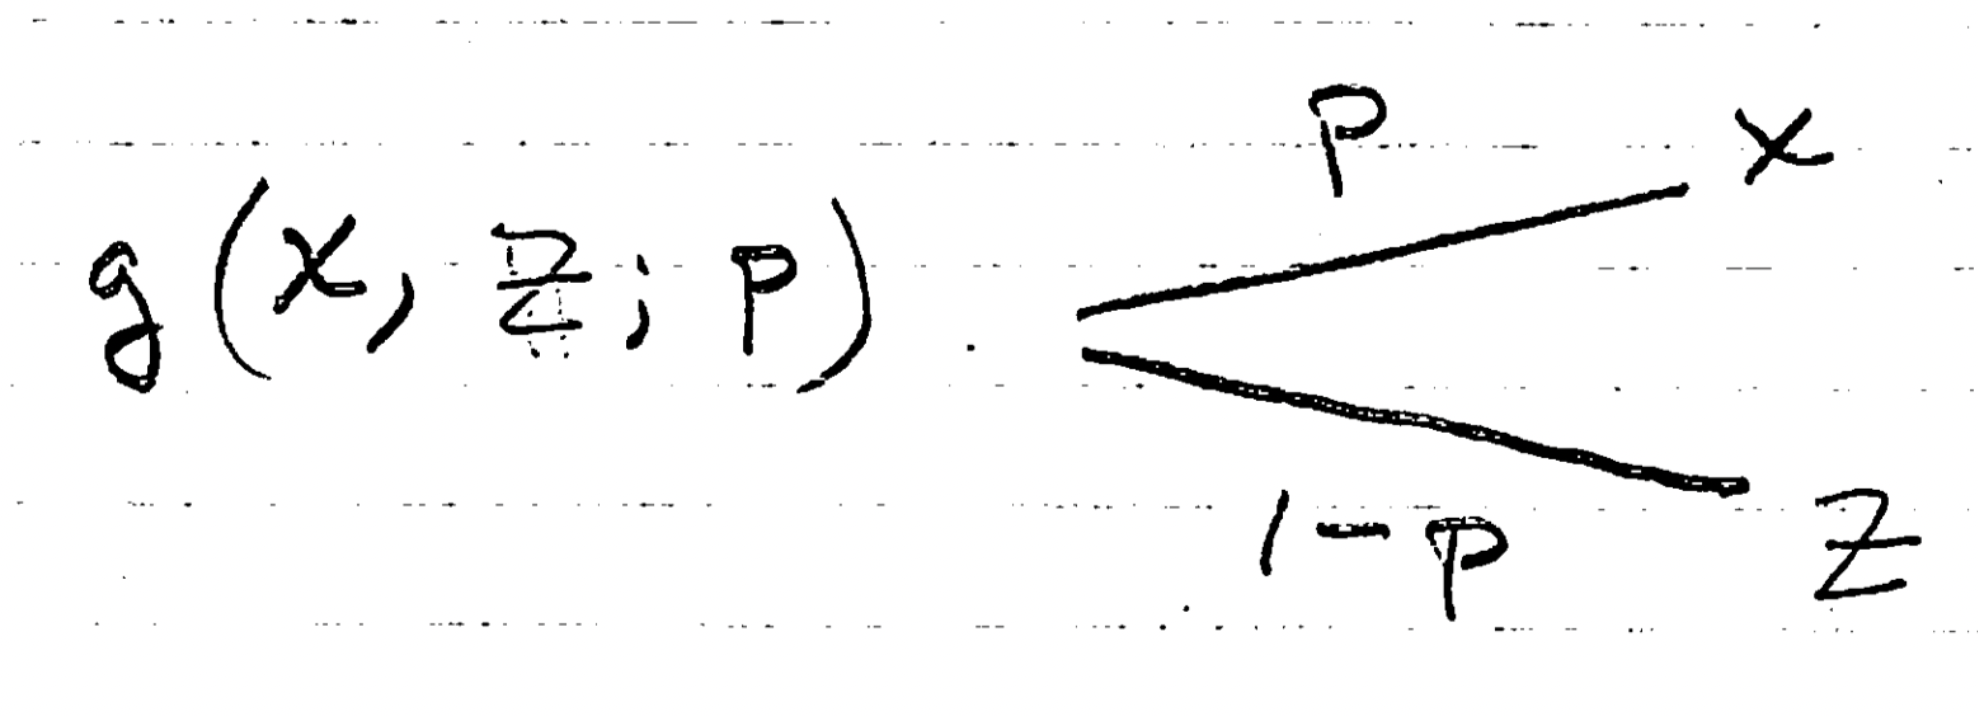
\includegraphics[width=0.7\textwidth]{L2-gamble}
    \centering
\end{figure}
\begin{align*}
    \textit{If }x &\sim y\\
    \textit{Then }g(x,y;p) &\sim g(y,z;p)\\
\end{align*}
\end{frame}

\begin{frame}
Axioms governing investors' behavior\\
\hfill \break
\textbf{A4 (Continuity)}: If $x \succsim y \succsim z$ then there exists a probability $p$ (unique unless $x \sim y \sim z$) such that\\
\hfill \break
\begin{align*}
    y &\sim g(x,z;p)\\
\end{align*}
\end{frame}

\begin{frame}
Axioms governing investors' behavior\\
\hfill \break
\textbf{A5 (Dominance)}:
\begin{align*}
    \textit{If }\;\;x \succsim y \succsim z,&\;\; x \succsim t \succsim z\\
    \textit{and }\;\;y \sim g(x,z;p_1),&\;\; t \sim g(x,z;p_2)\\
\end{align*}
\begin{align*}
    \textit{Then }\;\;p_1 > p_2 \implies& y \succ t\\
    \textit{and }\;\;p_1 = p_2 \implies& y \sim t\\
\end{align*}
\end{frame}

\subsection{Derivation}

\begin{frame}
\underline{\textbf{Derivation}}:\\
\hfill \break
Consider a set of (simple) gambles $g(M,m;h)$, that is, the payment $M$ with probability $h$ and $m<M$ with probability $1-h$.\\
From A4 (Continuity) we have $W_i\;\epsilon\;(m,M)$ such that\\
\[W_i \sim g(M,m;h(W_i))\]
\hfill \break
$W_i$ is the certainty equivalent of the gamble.
\end{frame}

\begin{frame}
We can construct the indifference set for $h=(0,1)$, (for a given individual)\\
\begin{figure}[indiff-set]
    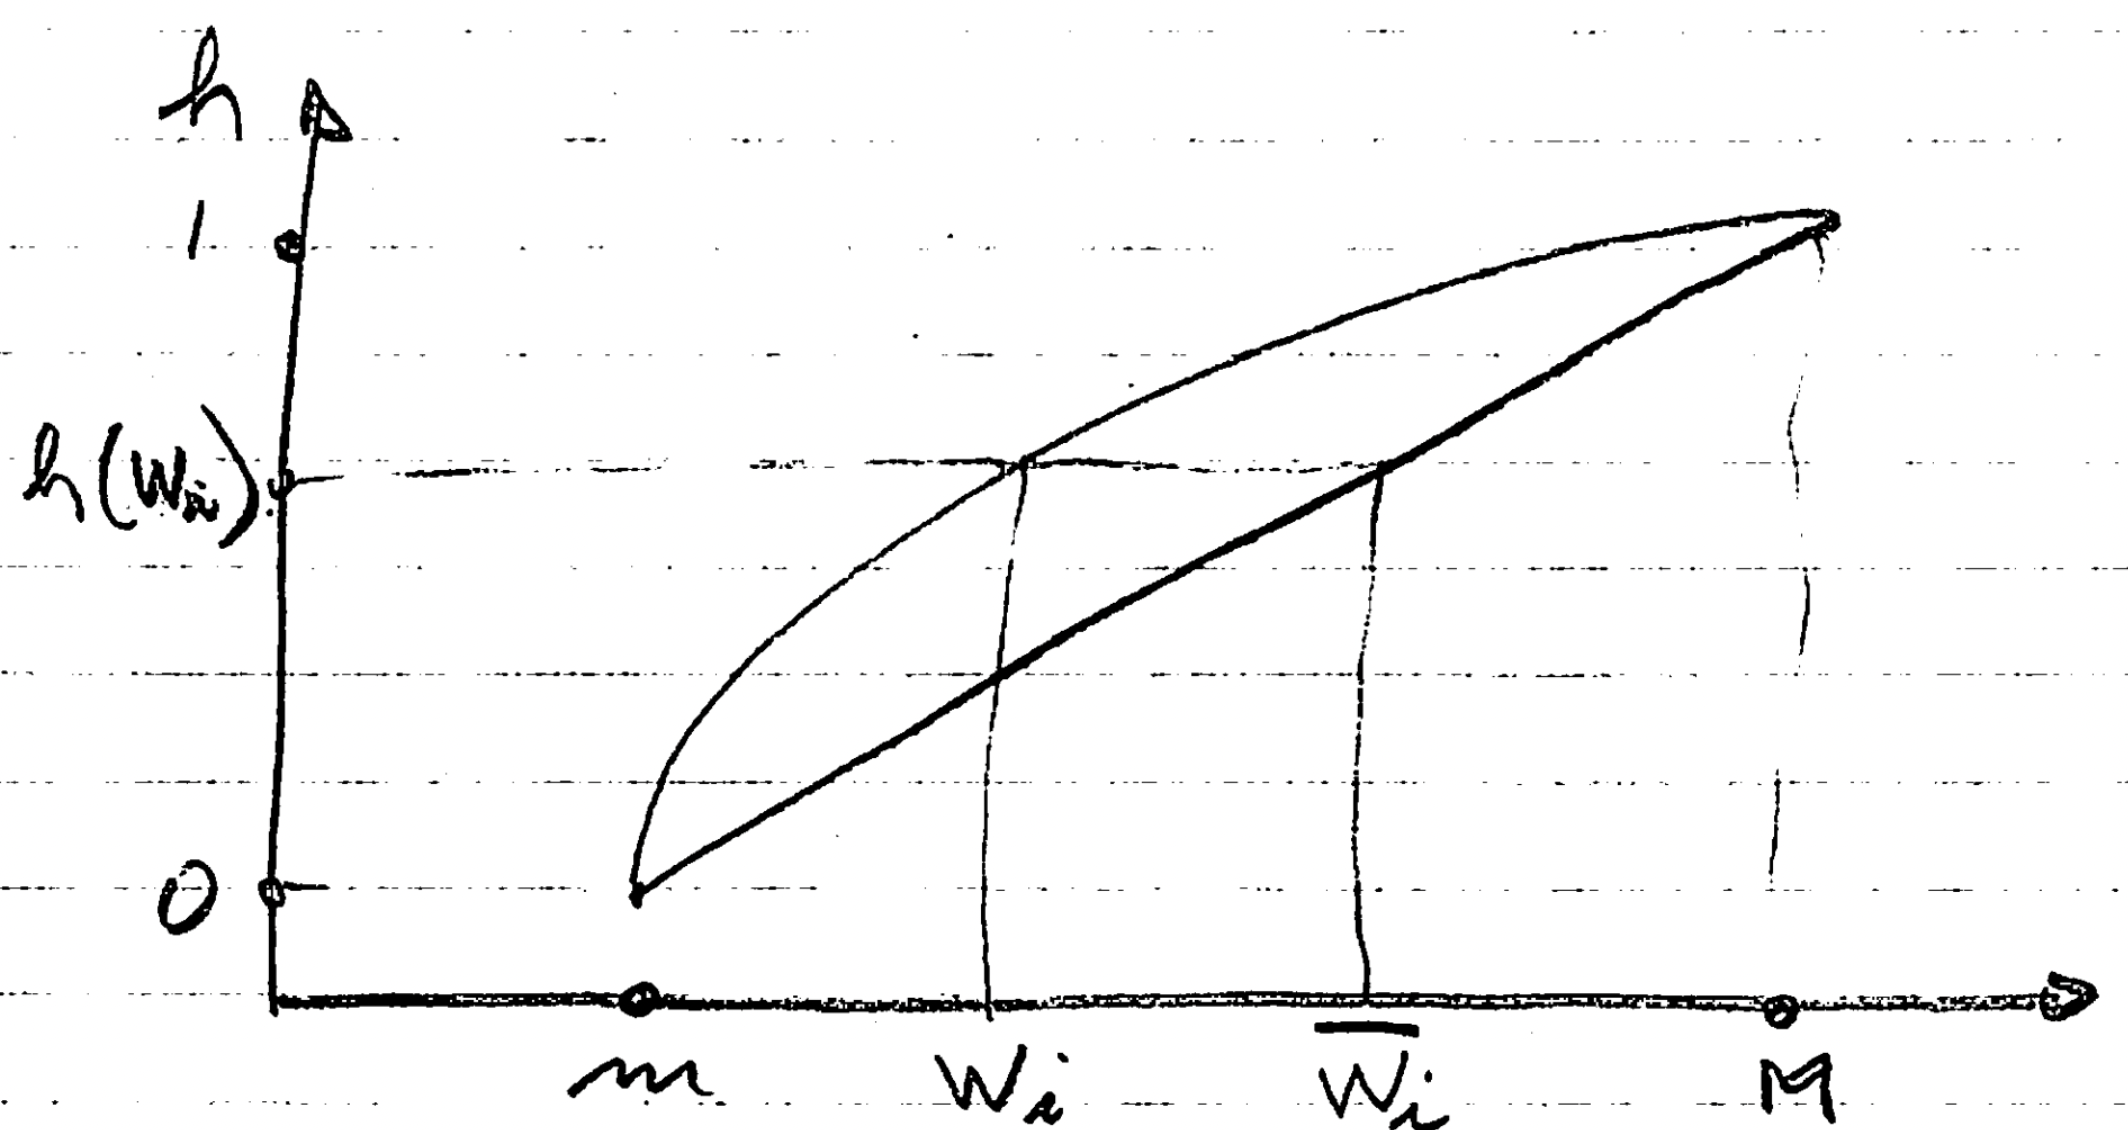
\includegraphics[width=0.6\textwidth]{L2-indiffset}
    \centering
\end{figure}
\[\bar{W}_i = hM+(1-h)m\]
For this preference function (concave) CE < expected value of the gamble ($W_i<\bar{W_i}$)
\end{frame}

\begin{frame}
Consider a (complex) gamble with payoffs $X_i$ with probabilities $p_i$, $i=1,...,n$\\
\begin{figure}[complex-gamble]
    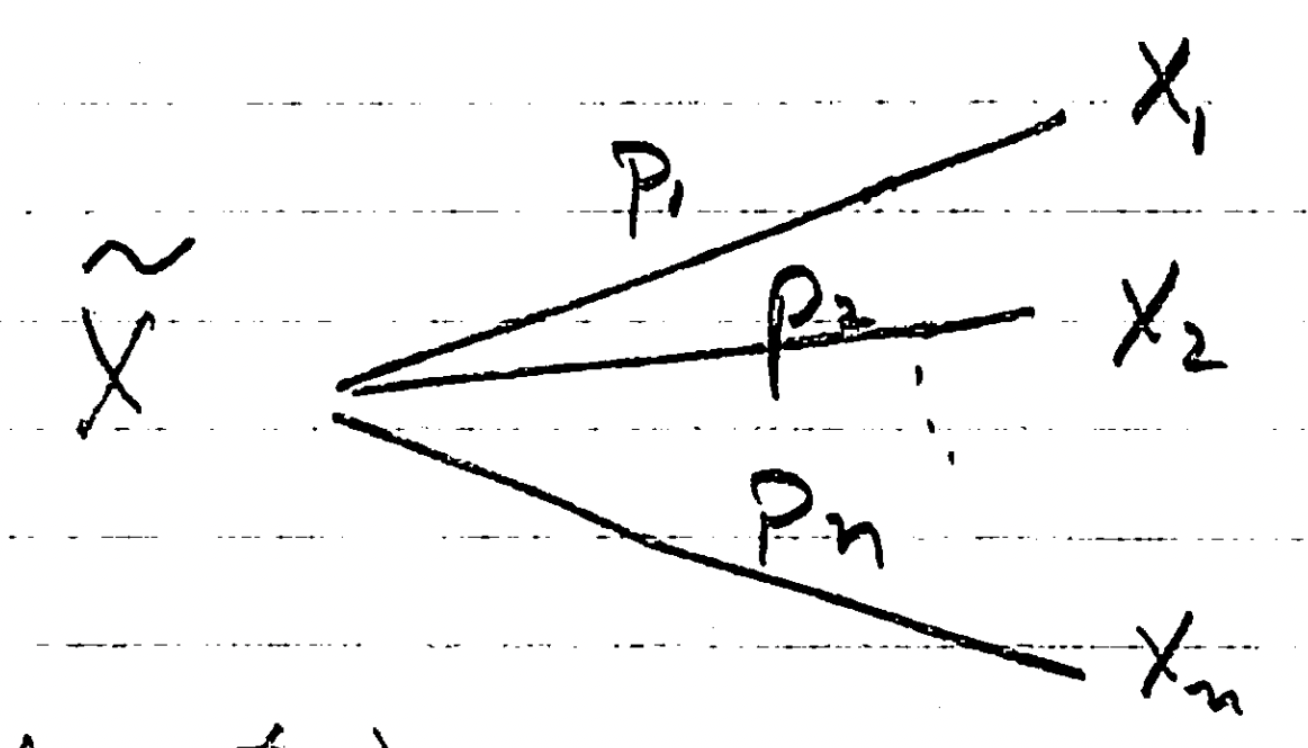
\includegraphics[width=0.5\textwidth]{L2-complex-gamble}
    \centering
\end{figure}
By A4 (Continuity) we can find $h_i$ such that $X_i \sim g(M,m;h_i)$...
\end{frame}

\begin{frame}
By A3 (Independence)\\
\begin{figure}[equivalence]
    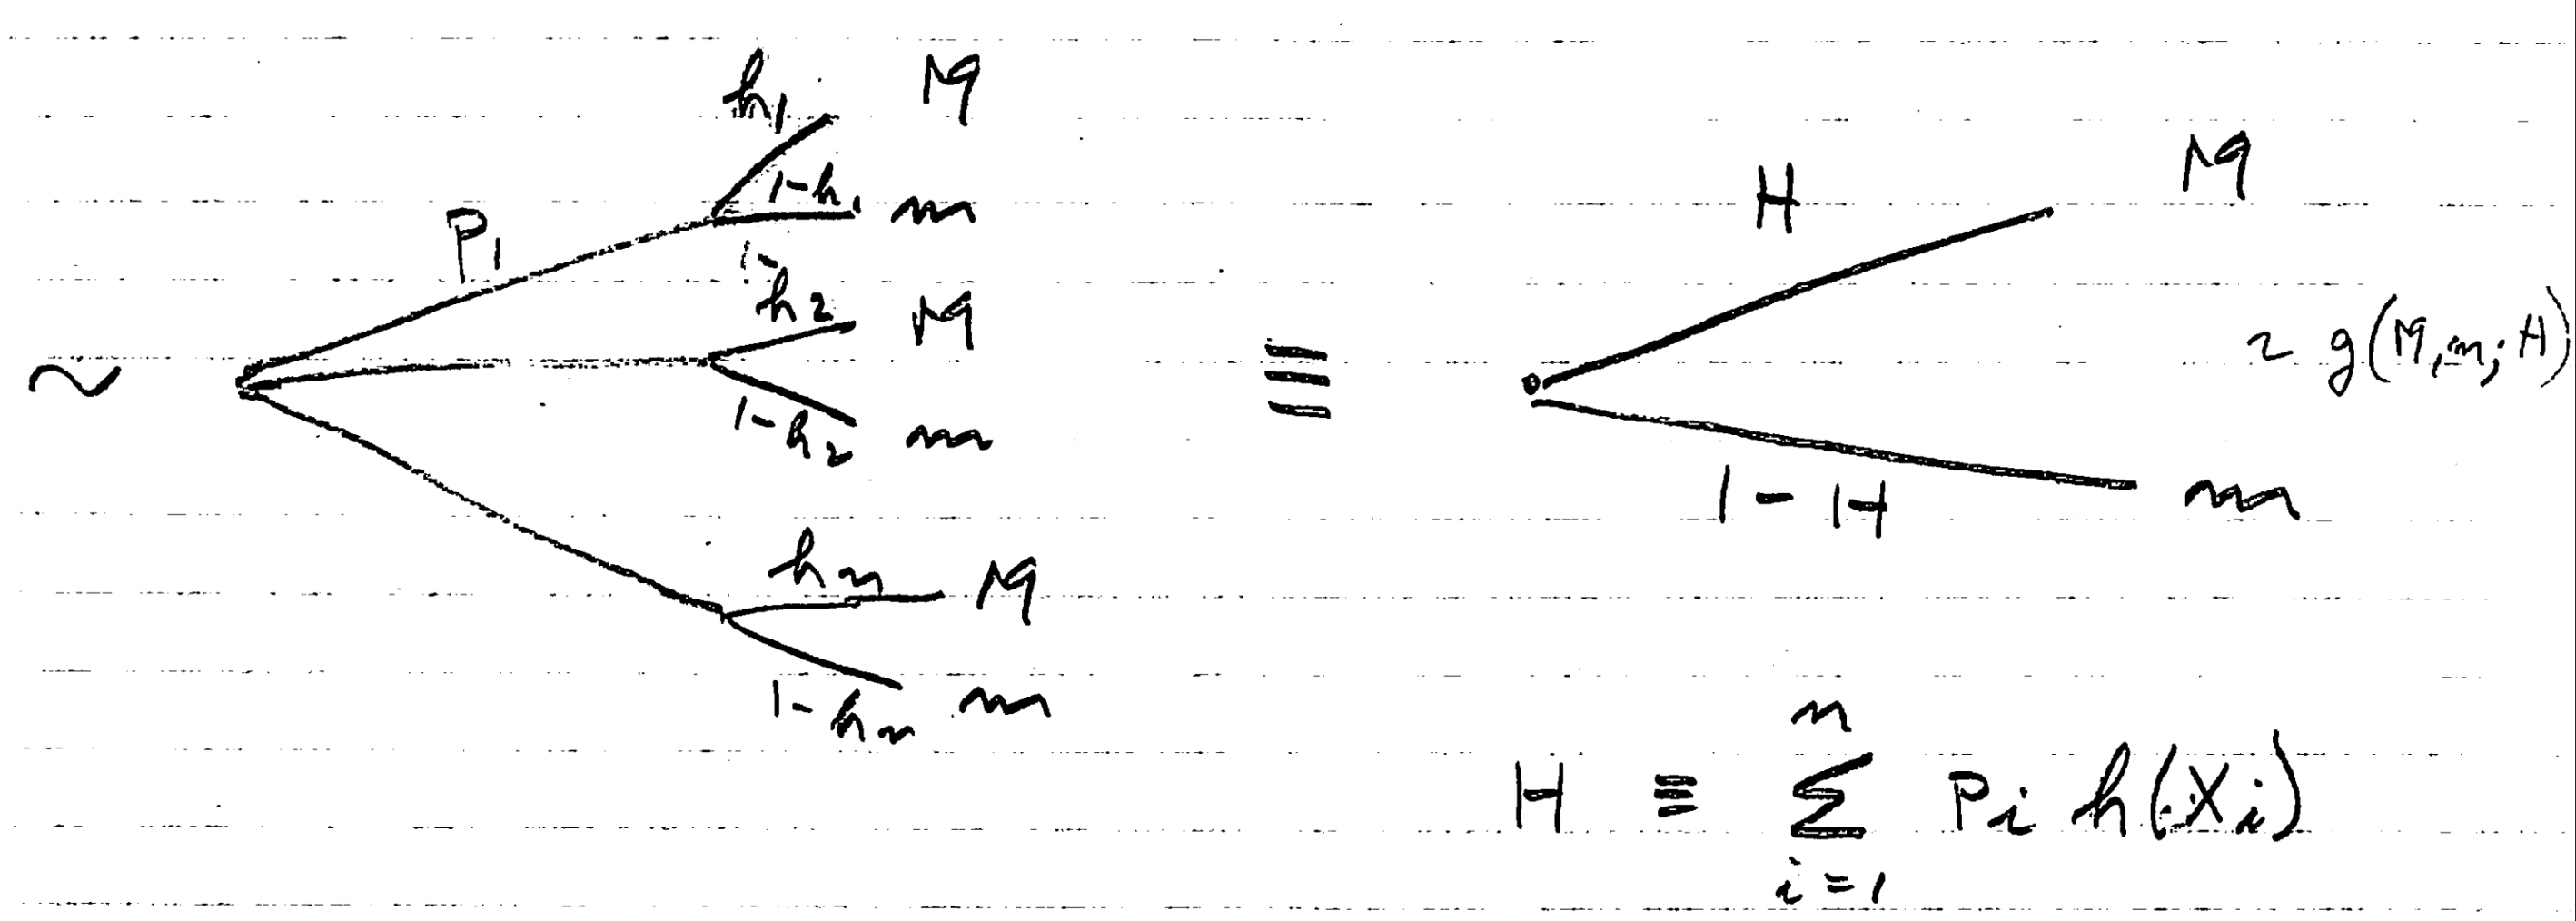
\includegraphics[width=1\textwidth]{L2-equivalence}
    \centering
\end{figure}
\end{frame}

\begin{frame}
Consider a second (complex) gamble with outcomes $Y_i$ and probabilities $q_i$, $i=1,...,N$\\
Then this gamble is equivalent to $g(M,m;Q)$
for
\[Q \equiv \sum_{i=1}^N q_i\;h(Y_i)\;\;,\;\;Y_i\sim g(M,m;h(Y_i))\]
\begin{align*}
    \therefore \;\; \Tilde{X}&\sim g(M,m;H)\\
    \Tilde{Y}&\sim g(M,m;Q)\\
\end{align*}
From A5 (Dominance) $\Tilde{X} \succ \Tilde{Y}$ iff $H > Q$ ...
\end{frame}

\begin{frame}
...we can write the probabilities $h(X_i) = u(x)$\\
\[\therefore \;\; \Tilde{X}\succ\Tilde{Y}\;\; \textit{ iff }\;\; E[u(x)]>E[u(y)]\]
\begin{center}
    \textbf{This is the expect utility theorem}\\
\end{center}
\hfill \break
The same preference ordering can be obtained by:\\
\[v(x)=a\;u(x)+b \;\;\;\; a,b \textit{ constants; } a>0\]
$\implies$ unique up to a positive linear transformation.\\
(Note: Interpersonal comparisons of utility are not possible.)
\end{frame}

\begin{frame}
\[v(x)=a\;u(x)+b \;\;\;\; a,b \textit{ constants; } a>0\]
\hfill \break
\underline{\textbf{b}} determines the origin and \underline{\textbf{a}} determines the scale of the utility measures (but they don't change the preference ordering).\\
\hfill \break
This should not be surprising because the selection of $\$m$ and $\$M$ were an arbitrary two points in the utility function.
\end{frame}

\subsection{Certainty Equivalent}

\begin{frame}
Certainty equivalent $W_c$ for complex gambles:
\[W_c \sim g(M,m;H)\]
\[\textit{ie. } u(W_c) = E[u(\textit{complex gamble}]\]
\hfill \break
If $\bar{W}$ is the expected outcome, then the individual is said to be:
\begin{align*}
    \textit{risk-averse if } W_c &< \bar{W} \impliedby u''<0\\
    \textit{risk-neutral if } W_c &= \bar{W} \impliedby u''=0\\
    \textit{risk-seeking if } W_c &> \bar{W} \impliedby u''>0\\
\end{align*}
It is easy to show this by Taylor's Theorem...
\end{frame}

\begin{frame}
\begin{align*}
    \textit{risk-averse if } W_c &< \bar{W} \impliedby u''<0\\
    \textit{risk-neutral if } W_c &= \bar{W} \impliedby u''=0\\
    \textit{risk-seeking if } W_c &> \bar{W} \impliedby u''>0
\end{align*}
By Taylor's Theorem:
\begin{align*}
    E[u(W)] &= E[u(\bar{W}+(W-\bar{W}))]\\
    &= E\bigg[u(\bar{W})+u'(\bar{W})(W-\bar{W})\\
    &\;\;\;+\frac{1}{2}u''(\bar{W}(1-\theta)+\theta W)(W-\bar{W})^2\bigg]\;\;\textit{for some }\theta, 0 \leq \theta \leq 1\\
    \therefore \;\; E[u(W)]-E[u(\bar{W})] &= u(W_c)-u(\bar{W}) = \frac{1}{2}E[u''(\cdot)(W-\bar{W})^2
\end{align*}
\end{frame}

\subsection{Example}
\begin{frame}
Risk Averse ($u''<0$)\\
\begin{figure}[l2-ra]
    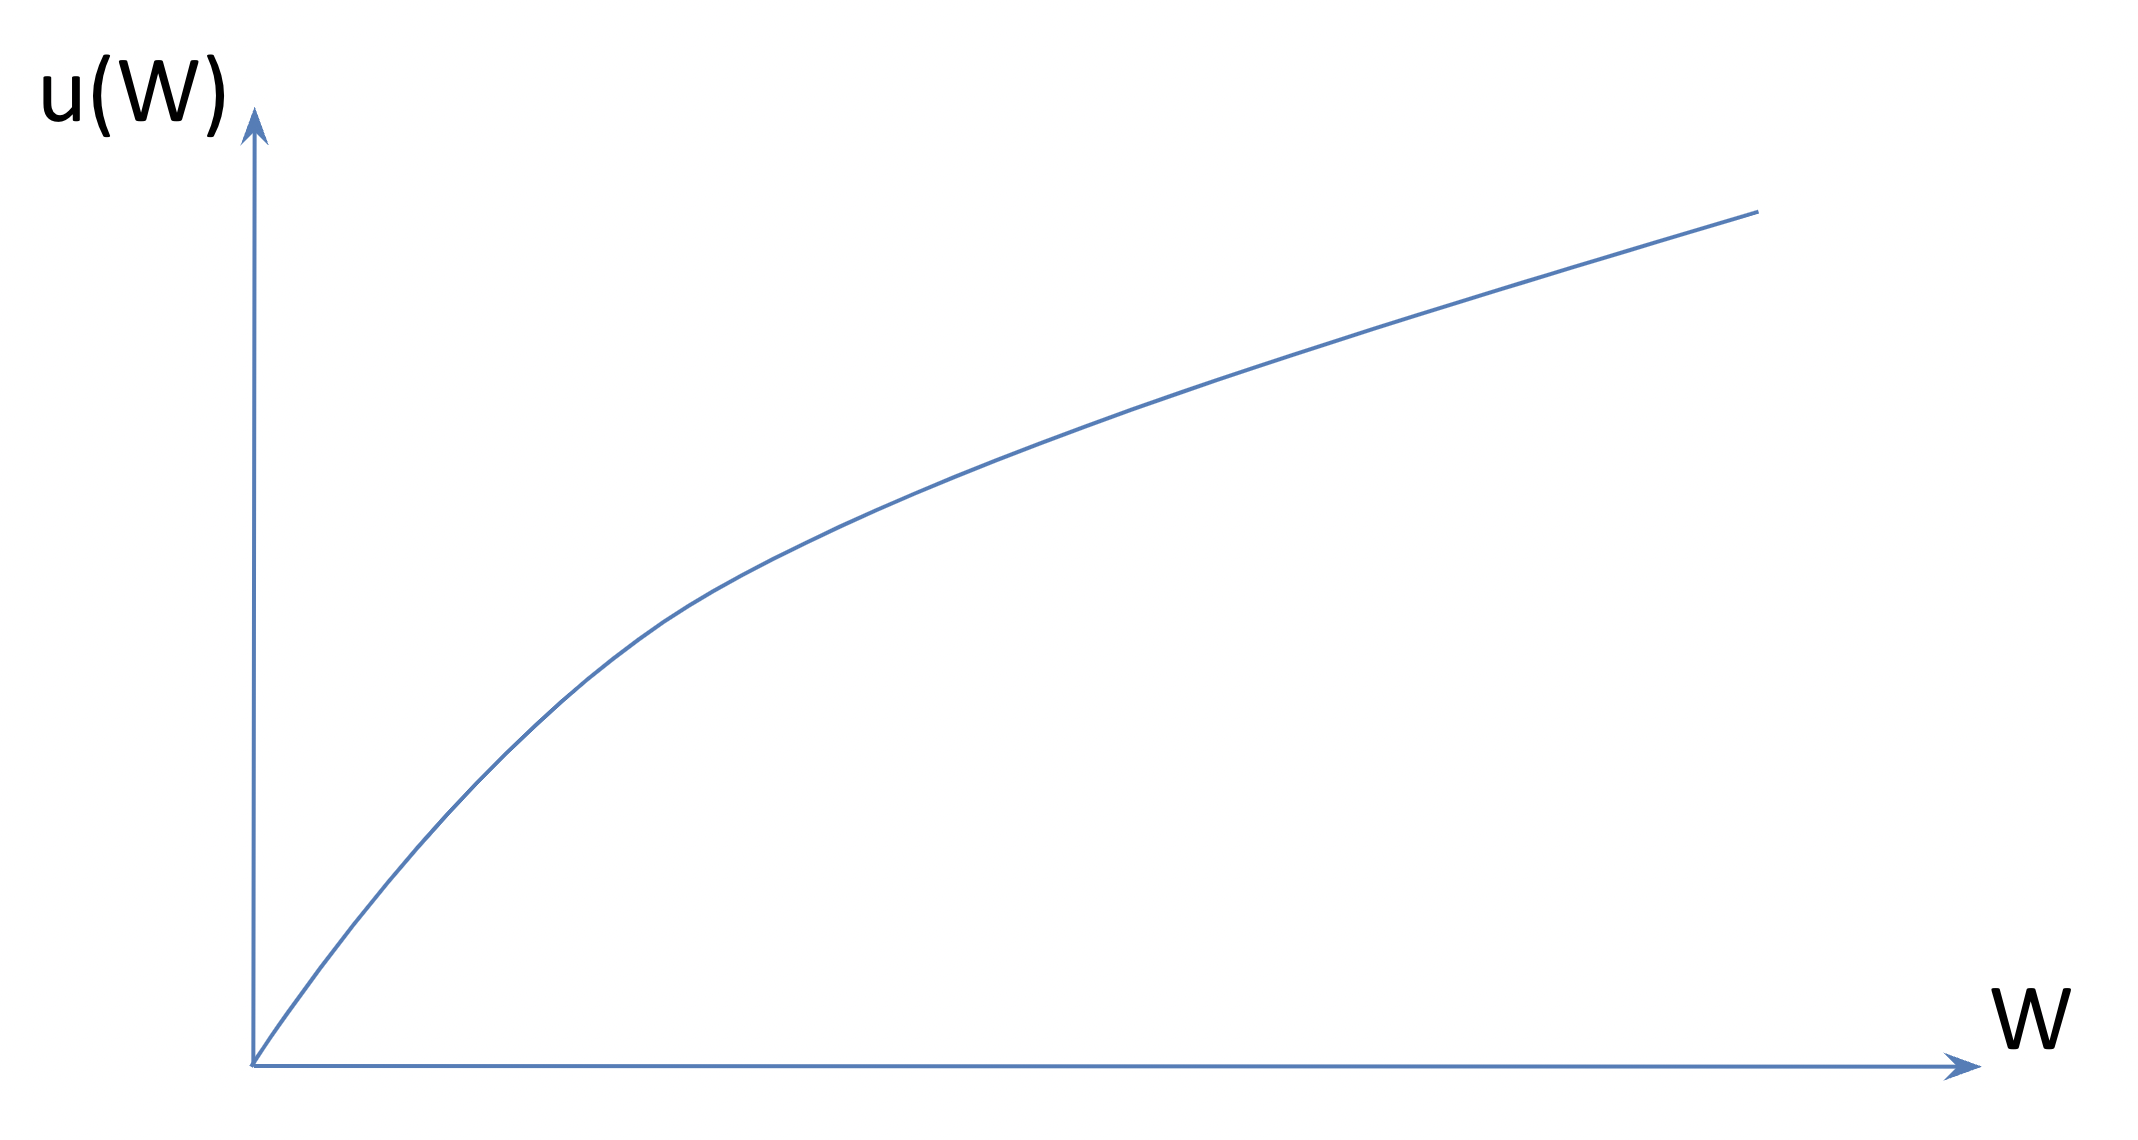
\includegraphics[width=0.7\textwidth]{L2-riskaverse}
    \centering
\end{figure}
Concave (Feel more "pain" to lose \$100 than pleasure to win) \$100.
\end{frame}

\begin{frame}
Risk Neutral ($u''=0$)\\
\begin{figure}[l2-rn]
    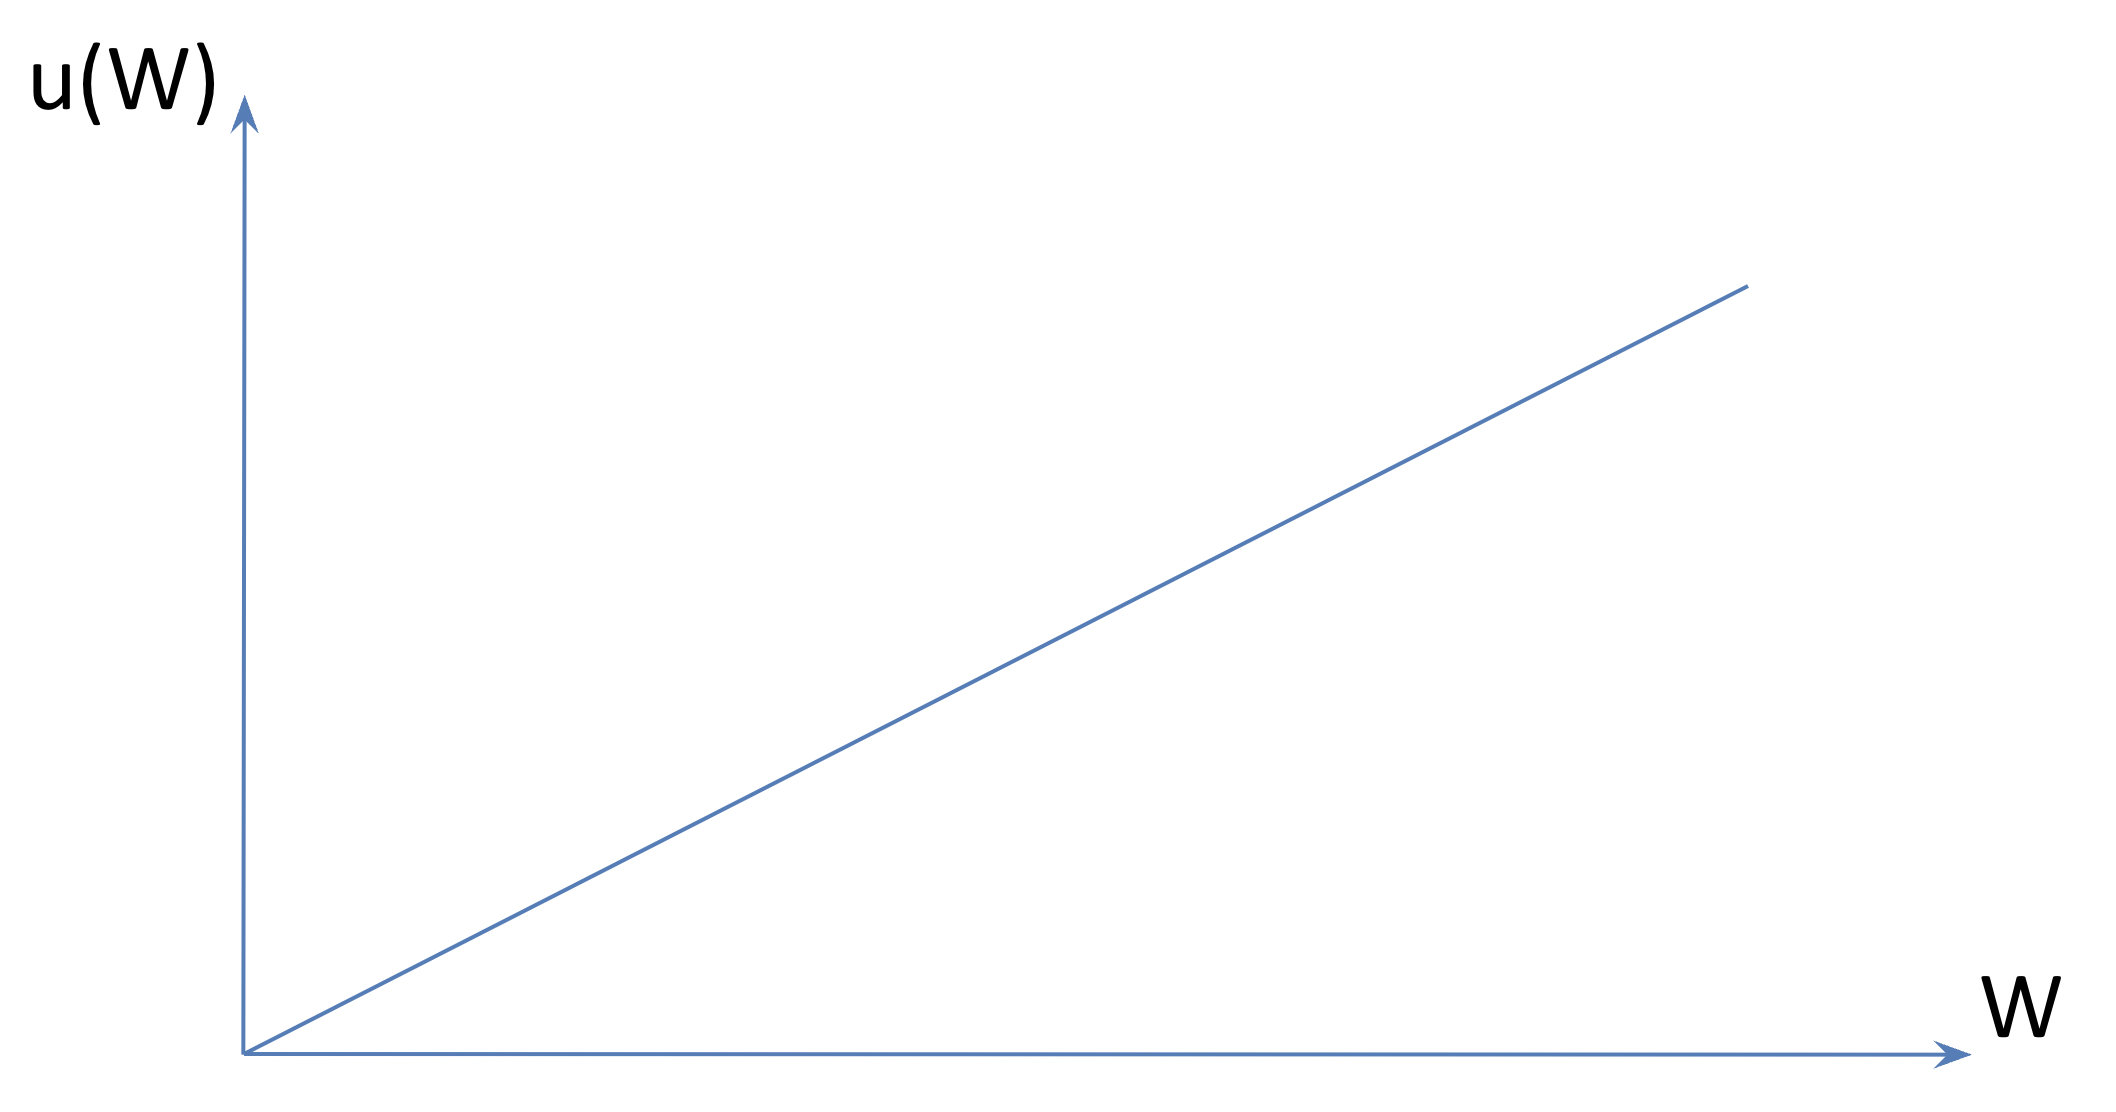
\includegraphics[width=0.7\textwidth]{L1-riskneutral}
    \centering
\end{figure}
Linear\\
\end{frame}

\begin{frame}
Risk Seeking ($u''>0$)\\
\begin{figure}[l2-rs]
    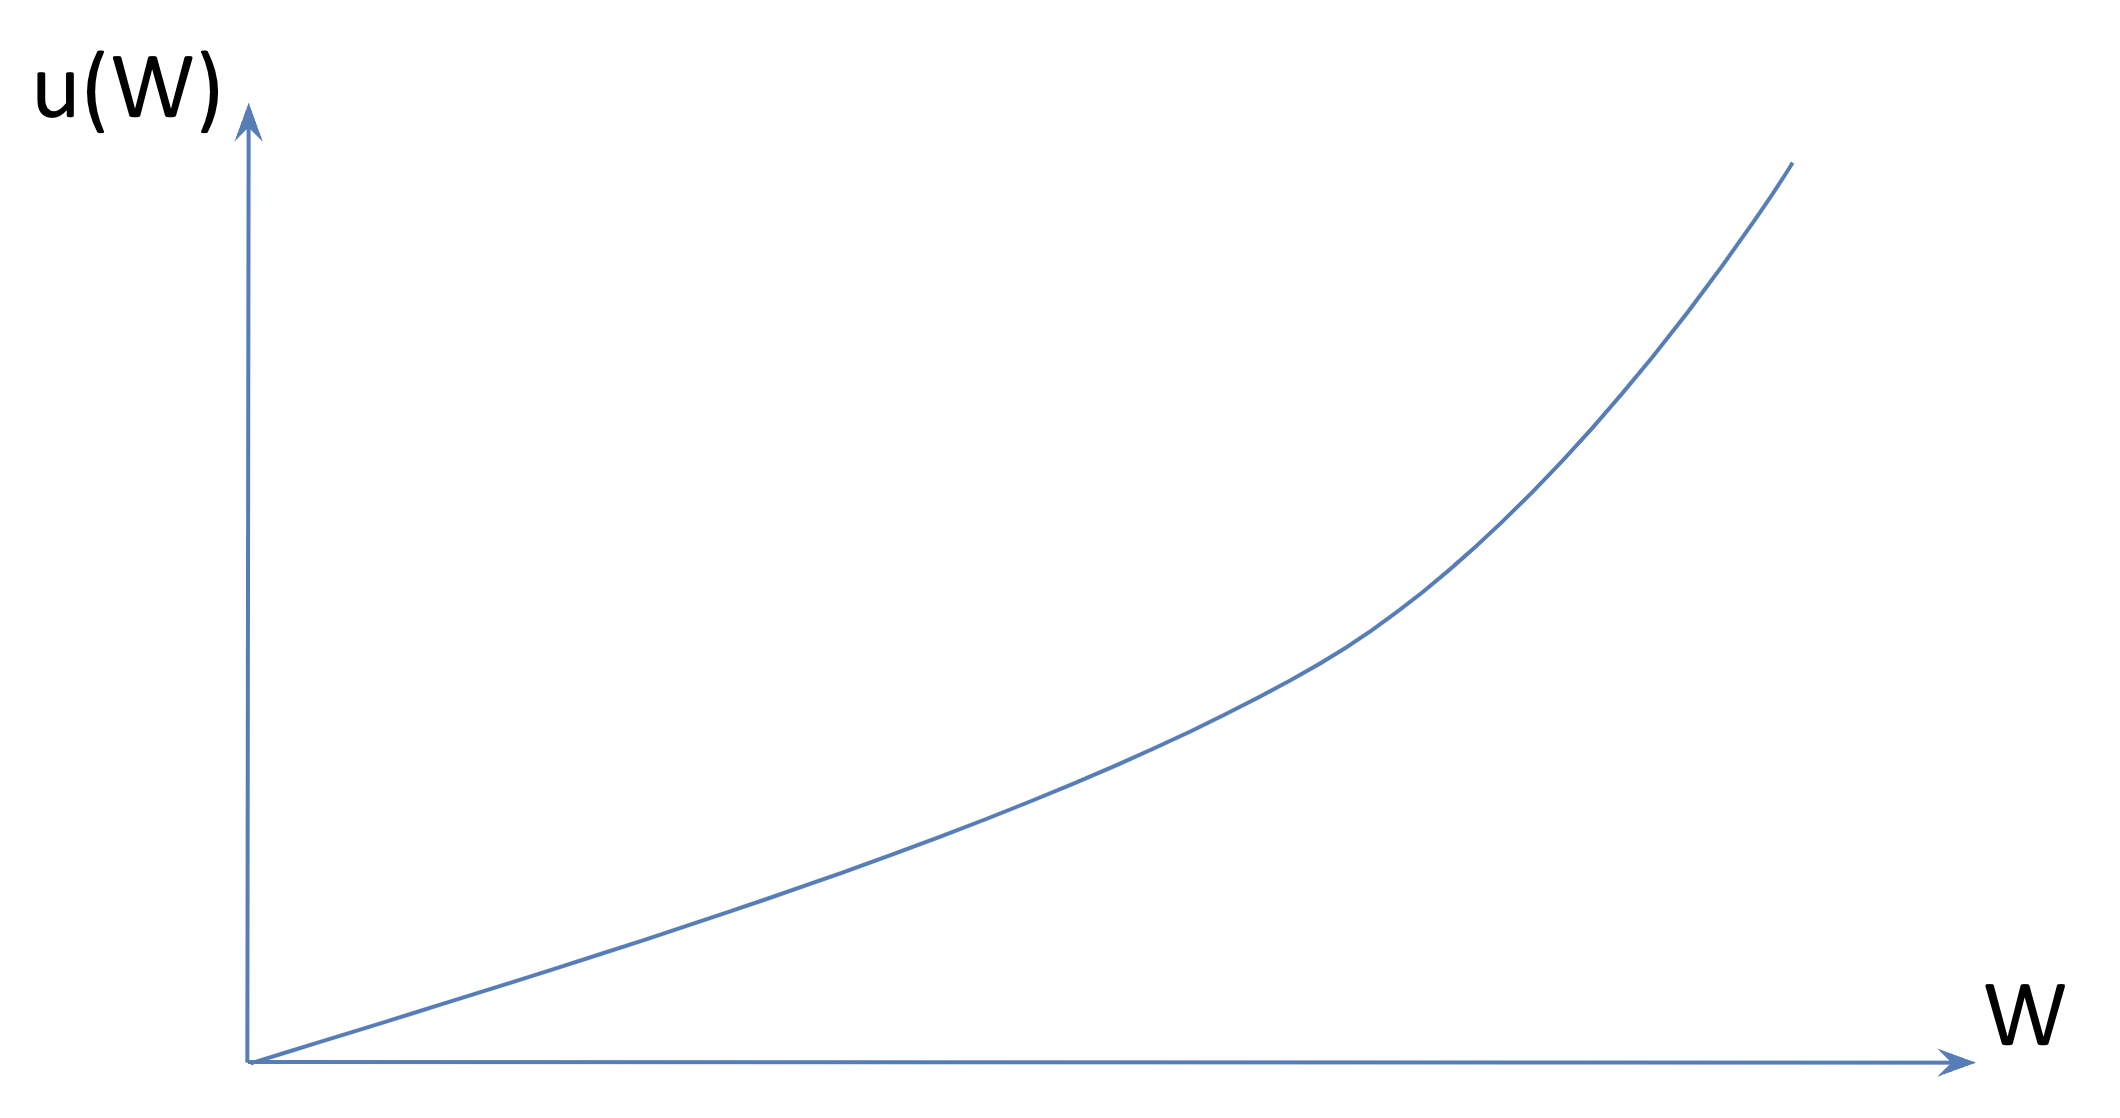
\includegraphics[width=0.7\textwidth]{L1-riskseeker}
    \centering
\end{figure}
Convex\\
\end{frame}

%%%%%%%%%%%%%%%%%%%%%%%%%%%%%%%%%%%%%%%%%%%%%%%%%%%%%
%%%%%%%%%%%%%% TOPIC 3  Risk Aversion %%%%%%%%%%%%%%%
%%%%%%%%%%%%%%%%%%%%%%%%%%%%%%%%%%%%%%%%%%%%%%%%%%%%%
\section{Risk Aversion}
\begin{frame}
We will assume that decision makers maximize expected utility of terminal wealth (one period model). Expected Utility Theorem: Von Neumann-Morgenstern utility function existence and uniqueness (if axioms of rational behaviour hold).\\
\hfill \break
\underline{risk averse}: if unwilling to accept every actuarially fair and immediately resolved gamble.\\
\[\textit{ie. } u(W) > E[u(W+\hat{\varepsilon})]\]
\[\textit{for all gambles with $E[\hat{\varepsilon}]=0$ and $\sigma_\varepsilon^2 >0$}\]
\hfill \break
\underline{globally risk averse}: if risk averse at all levels of wealth.\\
\end{frame}

\begin{frame}
Theorem: A necessary and sufficient condition for (global) risk aversion is a utility function of wealth that is strictly concave.\\
\hfill \break
Proof: if $u(\cdot)$ is strictly concave at W by Jensen's inequality (if $E[\varepsilon]=0$ actuarially fair)\\
\[ E[U(W+\tilde\varepsilon)] < U(E[W+\tilde\varepsilon]) = U(W)\]
\hfill \break
Actuarially Fair Gamble:\\
\[p\varepsilon_1+(1-p)\varepsilon_2 = 0\]
\[\varepsilon_1>0\;\;,\;\;\varepsilon_2<0\]
\end{frame}

\begin{frame}
Risk Averse\\
\[ E[u(W)+\tilde\varepsilon)] < U(E[W+\tilde\varepsilon]) = U(W)\]
\begin{align*}
    u(W) &= u(p(W+\varepsilon_1)+(1-p)(W+\varepsilon_2))\\
    &> p u(W+\varepsilon_1)+(1-p)u(W+\varepsilon_2)
\end{align*}
\begin{figure}[L3-riskaverse]
    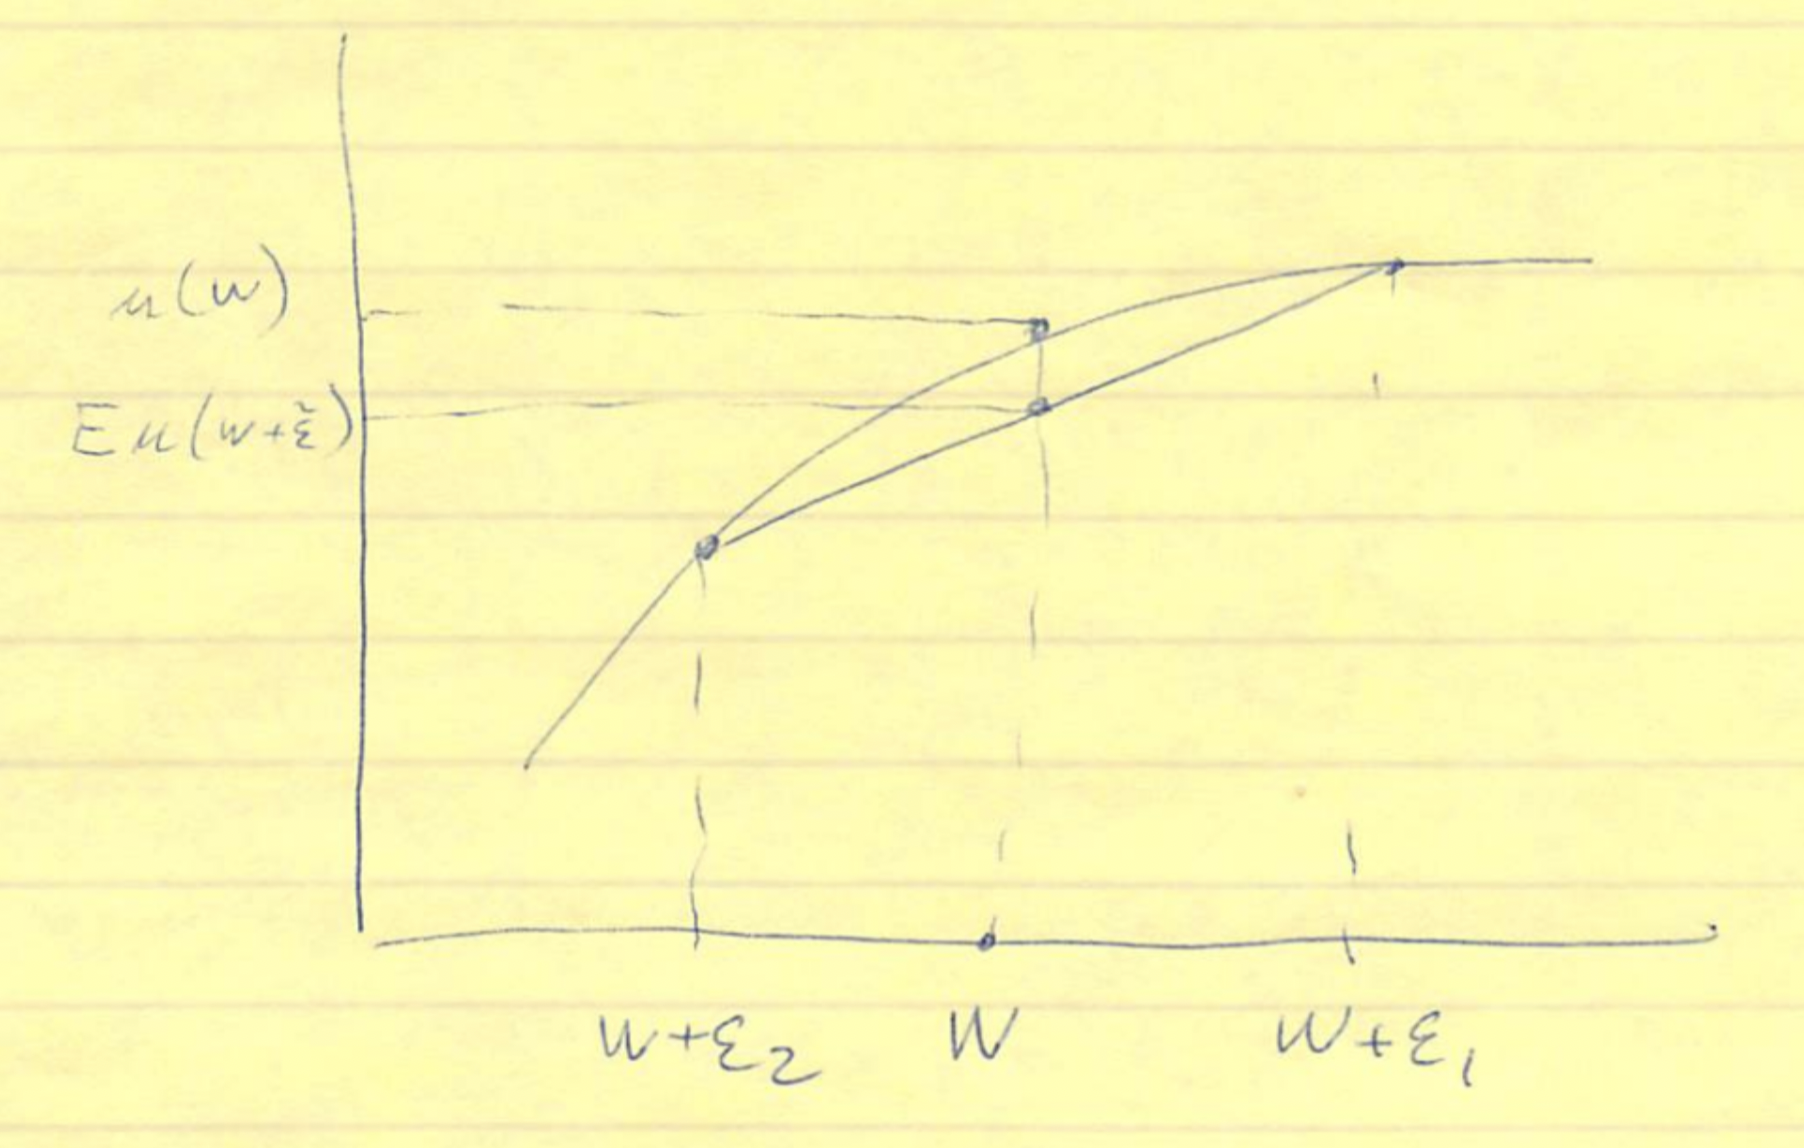
\includegraphics[width=0.5\textwidth]{L3-riskaverse}
    \centering
\end{figure}
\end{frame}

\begin{frame}
$\therefore$ risk averse $\implies$ concave utility function.\\
\hfill\break
A reversal of these steps demonstrates that concave utility function $\implies$ risk averse.\\
\begin{figure}[L3-riskaverse2]
    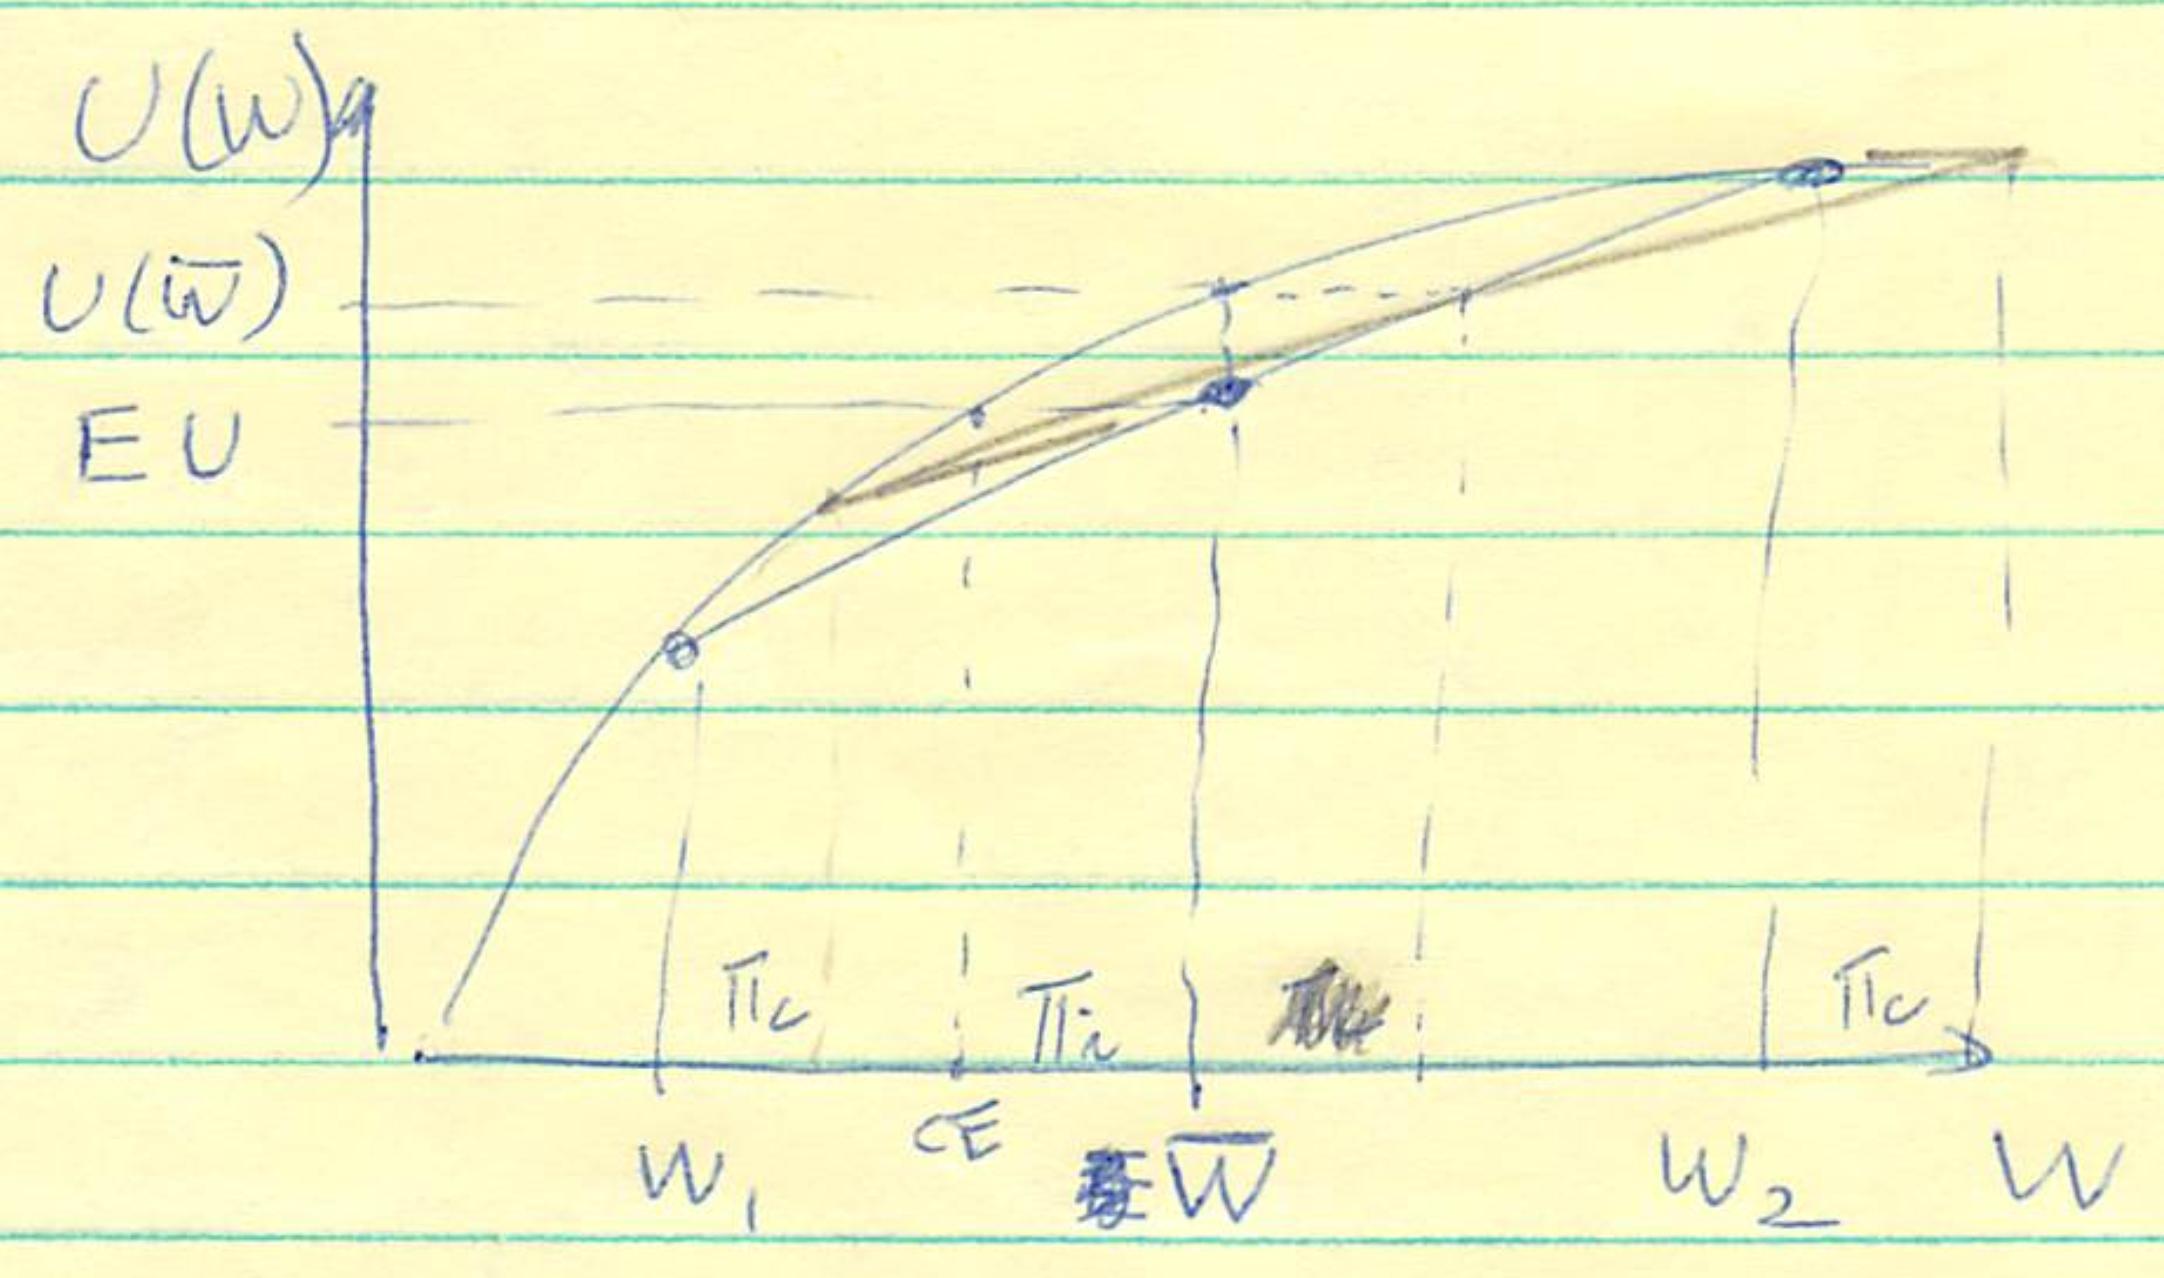
\includegraphics[width=0.5\textwidth]{L3-riskaverse2}
    \centering
\end{figure}
\begin{center}
    [to prove necessity, see Ingersoll]\\
    Concave $\iff$ $u''(W)<0$\\
\end{center}
\end{frame}

\begin{frame}
To avoid a gamble, a risk averse person would be willing to pay an \underline{insurance risk premium}, $\pi_i$ (used in economic analyses)\\
\hfill \break
1. $E[U(W+\tilde\varepsilon)] = U(W-\pi_i)$\\
\hfill \break
$W-\pi_i$: the certainty equivalent of gamble $W+\tilde\varepsilon$\\
To induce a risk averse investor to undertake a gamble, a \underline{compensatory} risk premium $\pi_C$ would have to be offered.\\
\hfill \break
2. $E[U(W+\pi_c+\tilde\varepsilon)] = U(W)$\\
\hfill \break
Used in financial applications, "extra" return expected on a riskier assets.\\
\hfill \break
The two premia are closely related but not identical. If utility function is smooth and risk is small, they are almost equal.\\
\end{frame}

\subsection{Measures of Risk Aversion}
\begin{frame}
The size of $u''(W)<0$ is not meaningful, $u'(W)>0$ more is preferred to less.\\
\hfill \break
Absolute Risk Aversion $\;\;A(W) = -\frac{u''(W)}{u'(W)}$\\
\hfill \break
Risk-Tolerance Function $\;\;T(W) = \frac{1}{A(W)}$\\
\hfill \break
Relative Risk Aversion $\;\;R(W) = W\cdot A(W)$\\
\hfill \break
All of these are independent of positive linear transformations of the utility function.\\
\[v(W)=a\cdot u(W)+b,\;\;a>0\]
Allows for comparisons between individuals.
\end{frame}

\subsection{Useful Utility Functions}
\begin{frame}
1. \underline{Constant Absolute Risk Aversion} ($A(W) = a$)\\
Only utility function $\iff$ exponential (up to two arbitrary constants).
\hfill \break
\begin{align*}
    u(W) =& -\frac{1}{a} e^{aW},\;\;a>0 \;\;\textit{for risk aversion}\\
    u' =& \;e^{-aW}\\
    u''=&\;-ae^{-aW}\\
\end{align*}
\begin{align*}
    A(W) = a&,\;\;A'(W) = 0\\
    R(W) = aW&,\;\;R'(W) = a > 0\\
\end{align*}
\end{frame}

\begin{frame}
2. \underline{Constant Relative Risk Aversion} $\iff$ power and logarithmic functions.\\
This family is also known as \underline{isoelastic} utility functions.\\
\begin{align*}
    u(W) =& \frac{W^{\gamma}}{\gamma}\;\;\gamma<1,\gamma\neq0\\
    =& \log(W)\;\;\gamma=0,\Bigg[\lim_{\gamma \to 0} \frac{W^\gamma-1}{\gamma}=\lim\frac{W^\gamma \ln{W}}{1}\Bigg]\\
\end{align*}
($u'=W^{\gamma-1}; u'' = (\gamma-1)W^{\gamma-2}$)\\
\begin{align*}
    A(W) = \frac{(1-\gamma)}{W}&,\;\;A'(W) = -\frac{(1-\gamma)}{W^2}<0\\
    R(W) = (1-\gamma)&,\;\;R'(W) = 0\\
\end{align*}
\end{frame}

\begin{frame}
3. \underline{Quadratic}: one of the theoretical justifications of the CAPM.\\
\hfill \break
\begin{align*}
    u(W) = W-\frac{1}{2}bW^2 &,\;\;0\leq W \leq \frac{1}{b}\\
    \Bigg(u' = 1-bW&, u''=-b\Bigg)\\
\end{align*}
\begin{align*}
    A(W) = \frac{b}{1-bW}&,\;\;A'(W) = A^2(W)>0\\
    R(W) = \frac{bW}{1-bW}&,\;\;R(W) > 0\\
\end{align*}
\end{frame}

\begin{frame}
4. \underline{HARA} (Hyperbolic Absolute Risk Aversion) or Linear Risk Tolerance\\
\hfill \break
\begin{align*}
    u(W) = \frac{1-\gamma}{\gamma}(\frac{\beta W}{1-\gamma}+\eta)^\gamma &,\;\;\beta>0,\gamma\neq1,\frac{\beta W}{1-\gamma}+\eta>0\\
\end{align*}
\begin{align*}
    A(W) = \Bigg[\frac{W}{1-\gamma}+\frac{\eta}{\beta}\Bigg]^{-1}&,\;\;\implies \frac{1}{A(W)} = a+bW \;\textit{"linear risk tolerance"}\\
    R(W) = W\cdot A(W) \;\;\;\;\;\; &A'(W)=-(1-\gamma)A^2(W) \;\;\;\;\;\; R'(W)=\frac{\eta}{\beta}A^2(W)\\
\end{align*}
\end{frame}

\begin{frame}
Useful property: gives demand curves for the risky assets which are linear in wealth.\\
\begin{center}
\begin{tabular}{ l l l }
 Exponential & $\eta = 1$ & $\gamma= -\infty$ \\ 
 Quadratic & & $\gamma = 2$ \\  
 Isoelastic & $\eta = 0$ & $\gamma < 1$ \\
 Generalized Logarithmic &  & $\gamma = 0$ \\
 Linear(risk neutral) &  & $\gamma = 1$
\end{tabular}
\end{center}
and,
\begin{align*}
    u'(W) &= \beta \bigg[\frac{\beta W}{a-\gamma}+\eta\bigg]^{\gamma-1}\\
    u''(W) &= \beta^2 \bigg[\frac{\beta W}{1-\gamma} + \eta\bigg]^{\gamma-2}\\
    -\frac{u''}{u'} &= \bigg[ \frac{W}{1-\gamma}+\frac{\eta}{\beta}\bigg]^{-1}\\
\end{align*}
\end{frame}

%%%%%%%%%%%%%%%%%%%%%%%%%%%%%%%%%%%%%%%%%%%%%%%%%%%%%%%%%%%
%%%%%%%%%%%%%% TOPIC 4  Portfolio Selection %%%%%%%%%%%%%%%
%%%%%%%%%%%%%%%%%%%%%%%%%%%%%%%%%%%%%%%%%%%%%%%%%%%%%%%%%%%
\section{Portfolio Selection Problem}
\subsection{Portfolio Selection Problem (Arrow)}
\begin{frame}
In its simplest form, we have the choice of investing wealth $w_0$ in a riskless asset (cash) and a risky asset with rate of return $\tilde z$. (Amount $0 \leq x \leq w_0$)\\
\hfill \break
Final Wealth:
\begin{align*}
    \tilde w =& w_0-x + x(\tilde z+1) = w_0 + x\tilde z\\
    \Bigg[\;\textit{if $r_f$}\;\;\;\; \tilde w =& (w_0-x)(1+r_f)+x(\tilde z+1) = w_0(1+r_f) + x(\tilde z - r_f) \Bigg]\\
\end{align*}
\begin{align*}
    \max_x \; E[u(\tilde w)] =& E[u(w_0+x\tilde z)] = f(x)\\
    \textit{1st order cond. }\;\;\;\; f'(x) =& E[u'(\tilde w)z]\\
    f''(x) =& E[u''(\tilde w)z^2] < 0 \;\;\;\;\implies f \textit{ concave}\\
\end{align*}
\end{frame}

\begin{frame}
Kuhn–Tucker conditions:
\begin{align*}
    &\frac{df}{dx} \boldsymbol\leq 0,\;\frac{df}{dx}\cdot x=0 \;\;\;\;\;\;\;\;\;\;\;\;\textit{the problem has a lower constraint, $0\leq x$}\\
    &\frac{df}{dx} \boldsymbol\geq 0,\;\frac{df}{dx}\cdot (w_0-x)=0 \;\;\;\;\textit{the problem has an upper constraint, $x\leq w_0$}\\
\end{align*}
\begin{figure}[threecases]
    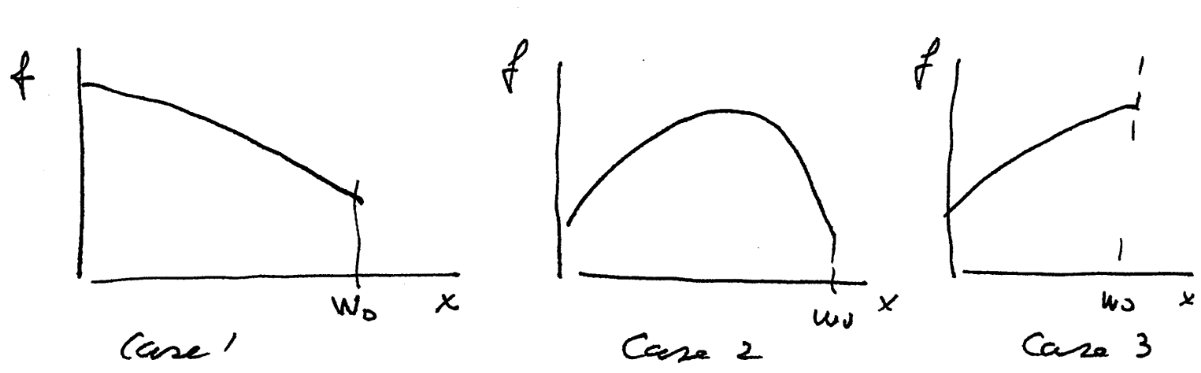
\includegraphics[width=0.8\textwidth]{L4-three-cases.png}
    \centering
\end{figure}
\end{frame}

\begin{frame}
\underline{Case 1}\\
\hfill \break
$\;\;\max\;f(x)$ at $x=0 \iff f'(x) \leq 0$\\
$\;\;\;\;\implies w=w_0$ and $u'(w) = u'(w_0) = \textit{constant}$\\
\begin{align*}
    \therefore \;\;\;\;&f'(0) = u'(w_0)E[z]\\
    &x=0 \iff E[z] \leq 0 \;\;\;\; [or\; E[z] \leq r_f]\\
    &x>0 \iff E[z] > 0\;\;\;\; \textit{independent of risk aversion}\\
\end{align*}
\underline{Case 3}\\
\[f'(w_0) = E[u'(w_0+w_0z)z] \geq 0\]
\end{frame}

\begin{frame}
\underline{Case 2:} Interior maximum at $f'(x^*)=0$\\
\[E[u'(w_0+x^*z)z] = 0\]
\hfill \break
given $u(\cdot)$ and the distribution of $z$, this can be solved for $x^*$.\\
\hfill \break
\begin{itemize}
    \item How does $x^*$ change with $w_0$? \textit{(see next page: implicit fn. thm.)}\\
\end{itemize}
\[\frac{dx^*}{dw_0} = -\frac{\partial f'/\partial w_0}{\partial f'/\partial x^*} = \frac{E[u''(w)z]}{E[u''(w)z^2]}\;\;\;\;\textit{(where $u''(w) < 0$)}\]
\[\therefore \;\; sign(\frac{dx^*}{dw_0}) = sign(E[u''(w)z])\]
\end{frame}

\begin{frame}
\underline{Recall:} Implicit Function Theorem\\
\begin{align*}
    &g(x,y) = 0\\
    &\frac{dx}{dy} = -\frac{\partial g / \partial y}{\partial g / \partial x}\\
\end{align*}
\end{frame}

\subsection{Relationship between Utility Functions and Risk Aversion}
\begin{frame}
We will now show that \underline{decreasing} $A(w)$, that is $A'(w) < 0$, $\implies \frac{dx^*}{dw_0}>0$ (risky investment is a normal good).\\
\hfill \break
Decreasing $A(w)$ implies
\begin{align*}
    -\frac{u''(w)}{u'(w)} = A(w_0+xz) &\leq A(w_0)\;\;\;\;\textit{for $z \geq 0$}\\
    \therefore \;\; u''(w_0+xz) &\geq -A(w_0)\cdot u'(w_0+xz)\\
    \textit{mult by $z \geq 0$} \;\;\;\; u''(w_0+xz)z &\geq -A(w_0)\cdot u'(w_0+xz)z\\
\end{align*}
and the same inequality holds for $z \leq 0$...
\end{frame}

\begin{frame}
\begin{align*}
    \therefore \;\; E[u''(w)z] &\geq -A(w_0)\cdot E[u'(w)z] >= 0\\
    \therefore \;\; \textit{decreasing }A(w) &\implies \frac{dx^*}{dw_0}>0 \;\;\;\;\textbf{(power)}\\
    \textit{constant }A(w) &\implies \frac{dx^*}{dw_0}=0 \;\;\;\;\textbf{(exponential)}\\
    \textit{increasing }A(w) &\implies \frac{dx^*}{dw_0}<0 \;\;\;\;\textbf{(quadratic)}\\
\end{align*}
\end{frame}

\begin{frame}
By defining $x = \alpha w_0$ as a fraction of wealth,
\[\tilde w = w_0 + \alpha w_0 \tilde z = w_0(1+\alpha \tilde z)\]
we could have proven similar results for $R(w)$.
\begin{align*}
    \textit{decreasing }R(w) &\implies \frac{d\alpha^*}{dw_0}>0\\
    \textit{constant }R(w) &\implies \frac{d\alpha^*}{dw_0}=0 \;\;\;\;\textbf{(power, logarithmic)}\\
    \textit{increasing }R(w) &\implies \frac{d\alpha^*}{dw_0}<0 \;\;\;\;\textbf{(exponential, quadratic)}\\
\end{align*}
\end{frame}

\begin{frame}
\underline{Exponential Utility}
\[u(w) = -\frac{1}{a}e^{-aW}\]
\begin{align*}
    \textit{1st order condition:}\;\;\;\; E[e^{-a(w_0+x^*z)} \cdot z] &= 0\\
    f'(\cdot) = e^{-aW_0} &= 0\;\;\;\;\textit{where $x^*$ is independent of $w_0$}
\end{align*}
\begin{itemize}
    \item How does $x^*$ change with $a$?\\
\end{itemize}
\begin{align*}
    \frac{dx^*}{da} &= -\frac{\partial f'/\partial a}{\partial f'/\partial x^*} = -\frac{E[-z^2 x^*e^{-ax^*z}]}{E[-z^2 ae^{-ax^*z}]}\\
    \frac{dx^*}{da} &= -\frac{x^*}{a}<0 \;\;\;\; \textit{for $x^*>0$}
\end{align*}
The more risk averse (greater a) the investor, the less they will invest in a risky asset.
\end{frame}

\begin{frame}
\underline{Power Utility}
\[u(w) = \frac{w^\gamma}{\gamma} = u(w_0(1+\alpha z))\]
\begin{align*}
    E[(w_0(1+\alpha^*z))^{\gamma-1}\cdot w_0z] &= 0\\
    f'(\cdot) = E[(1+\alpha^*z)^{\gamma-1}\cdot z] &= 0\;\;\;\;\textit{where $\alpha^*$ is independent of $w_0$}
\end{align*}
\begin{itemize}
    \item How does $\alpha^*$ change with $\gamma$?\\
\end{itemize}
\begin{align*}
    \frac{d\alpha^*}{d\gamma} &= -\frac{\partial f'/\partial \gamma}{\partial f'/\partial \alpha^*} >0 \;\;\;\; \textit{for $\gamma<1$ and $\alpha^*>0$}\\
\end{align*}
the more risk averse the investor, the less proportion they will buy of a risky asset
\end{frame}

\begin{frame}
Argument of utility function $\rightarrow$ \underline{wealth}\\
\hfill \break
When is it independent of $w_0$ and depends only on the set of risky prospects, $\tilde y$?\\
\[iff\rightarrow u(w_0+\tilde y) = a u(\tilde y) + b\]
This is only satisfied by exponential and linear utility functions of wealth.\\
\hfill \break
In both cases we can substitute $w = y+w_0$, the order does not change ($A(x) = constant$)
\end{frame}

\subsection{Unbounded Utility Functions}
\begin{frame}
\underline{St. Petersburg Paradox}: "proves" risk aversion since the expected value of the gamble designed to pay $\$2^n$ if the first occurrence of "heads" is on the $n^{th}$ toss is a payout of $\infty$.\\
\hfill \break
In the same fashion, for any unbounded (from above) utility function, there exists a solution $w_n$ to $u(w)=2^n$ for all $n$. Thus, if we make the payoffs $u^{-1}(2^n)$, the value of the gamble to our risk averse individual...
\[\sum_{n=1}^\infty \frac{1}{2^n} \cdot u[u^{-1}(2^n)] = \sum_{n=1}^\infty \frac{1}{2^n} \cdot 2^n = \infty\]
\begin{itemize}
    \item Note: not all gambles can be compared (violates Axiom I Completeness). Eg. consider a payoff of $u^{-1}(3^n)$ instead of $u^{-1}(2^n)$\break$E[u]=\infty$ still, but clearly the former is better.
\end{itemize}
\end{frame}

\subsection{Multi-period Utility Functions}
\begin{frame}
Defined over the vector of consumption withdrawals from wealth.\\
\[u(\underline{c}) = u(c_0, c_1, ..., c_T)\]
It is often convenient to assume that utility is \underline{additively separable}, ie.\\
\[u(\underline{c}) = \sum_{t=0}^T u(c,t)\]
the level of consumption in any period does not affect the amount of utility derived from consumption in any other period.\\
\end{frame}

\begin{frame}
Here we can define the concept of \underline{time preference}\\
\[\rho(c,t) = \frac{\partial u/ \partial c(t)}{\partial u/ \partial c(t+1)} = \frac{U_c(c,t))}{U_c(c,t+1)}\]
\begin{align*}
    \textit{if }\;\;\;\; U(c,t) = f(t) U(c) \;\;&\rightarrow\;\; \rho(t) = \frac{f(t)}{f(t+1)}\\
    \textit{and if }\;\;\;\; \rho(t) = \rho\;\textit{constant } \;\;&\rightarrow\;\; f(t)=\rho^{-t}\\
\end{align*}
\[u(\underline{c}) = \sum_{t=0}^T \rho^{-t}U(c)\]
This is very common in economic problems. In this framework $\rho$ can be viewed as a \underline{personal discount factor for utility over time}. 
\end{frame}

%%%%%%%%%%%%%%%%%%%%%%%%%%%%%%%%%%%%%%%%%%%%%%%%%%%%%%%%%%%%%%%%%%%%%%%%%
%%%%%%%%%%%%%% TOPIC 5  Discrete Time Portfolio Selection %%%%%%%%%%%%%%%
%%%%%%%%%%%%%%%%%%%%%%%%%%%%%%%%%%%%%%%%%%%%%%%%%%%%%%%%%%%%%%%%%%%%%%%%%
\section{Discrete Time Portfolio Selection}
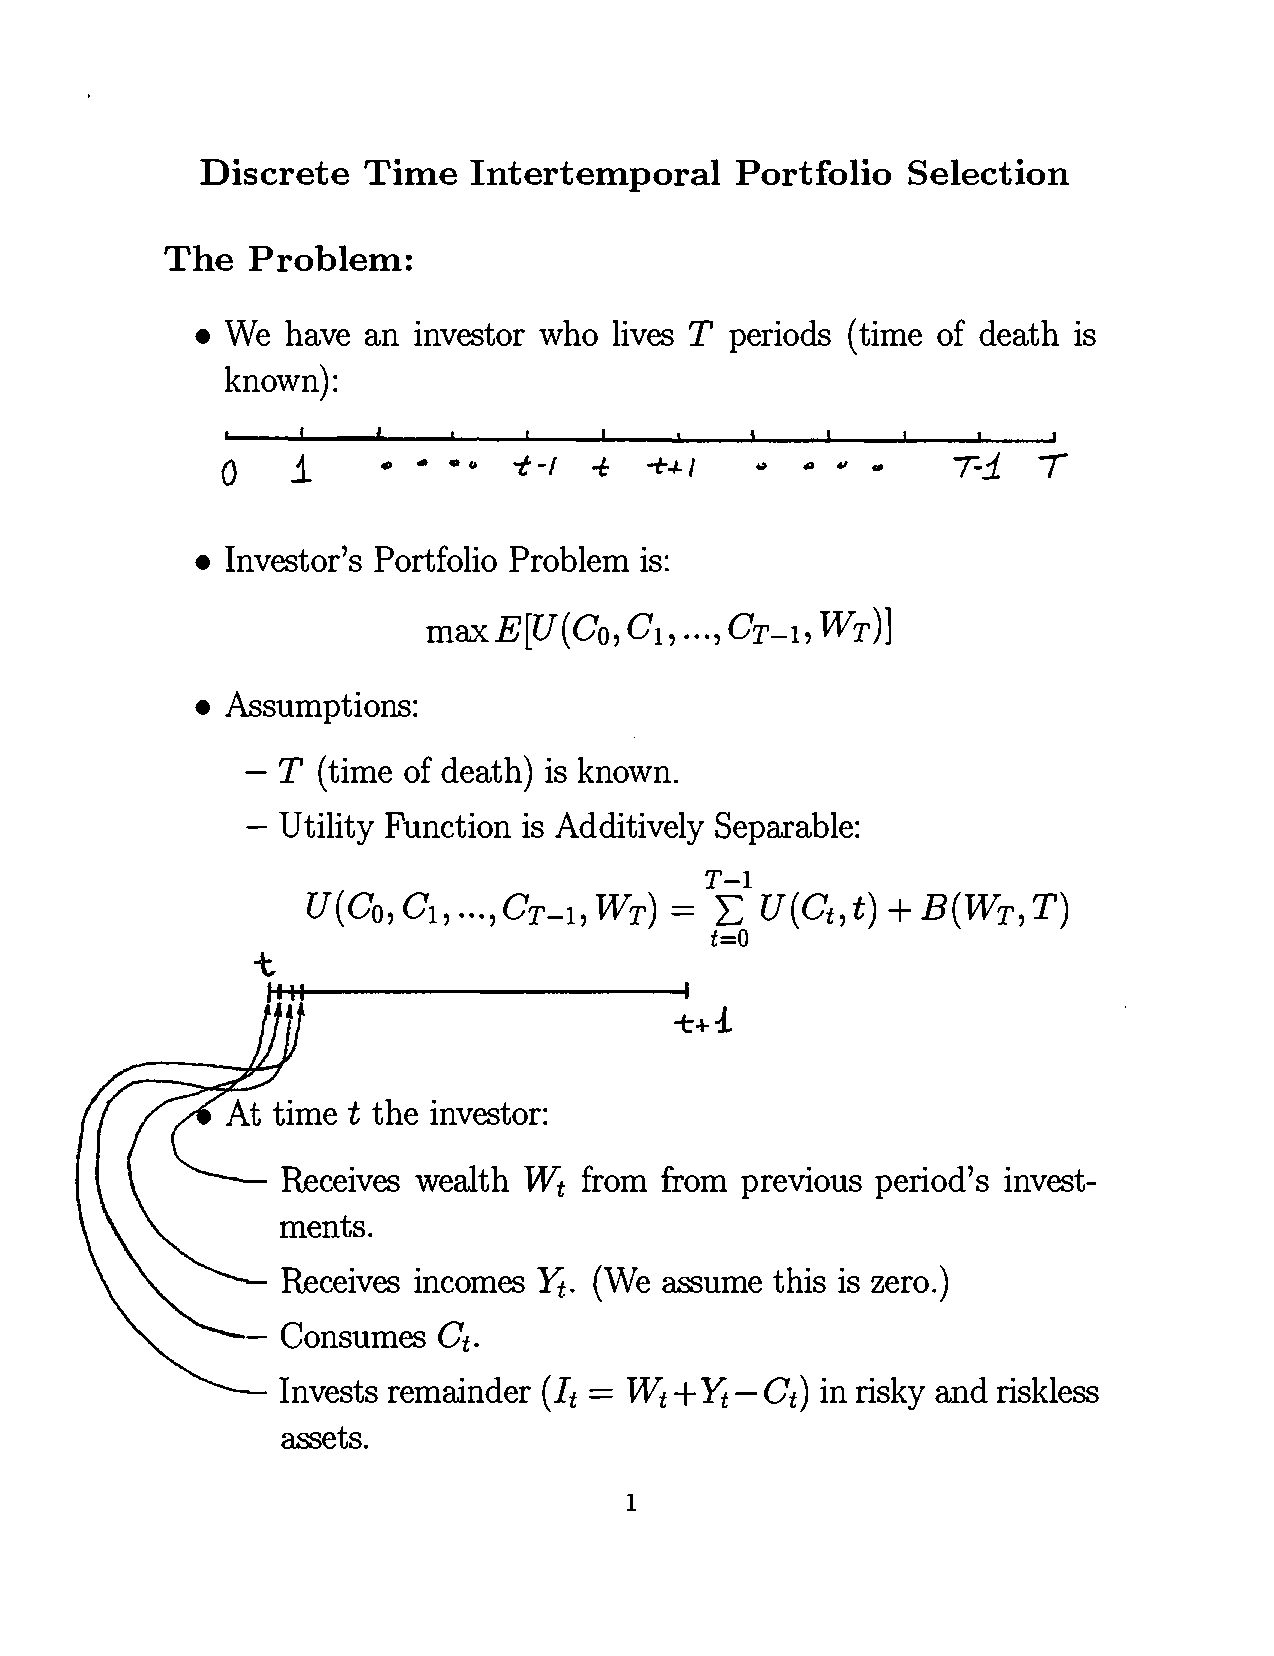
\includepdf[page={1-5}]{pdfs/topic5}

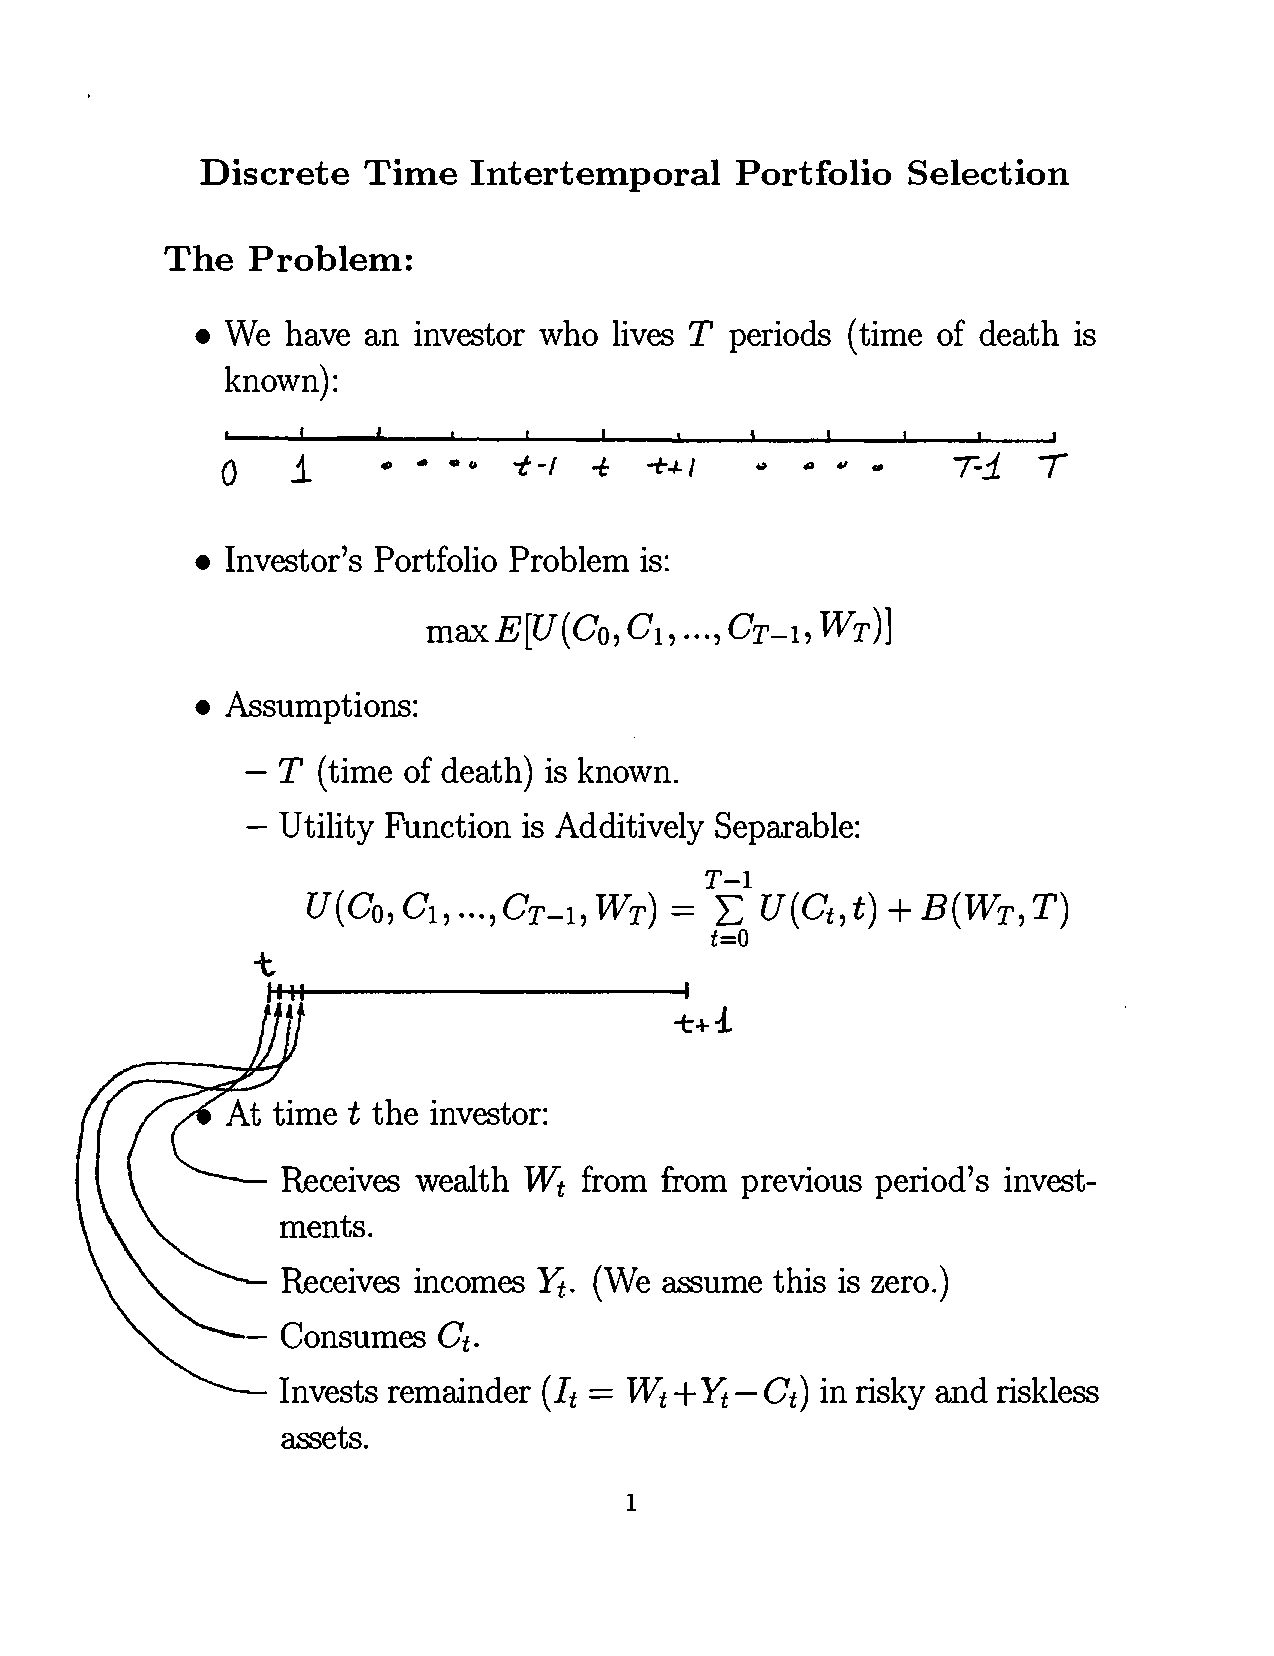
\includepdf[page={7-14}]{pdfs/topic5}

%%%%%%%%%%%%%%%%%%%%%%%%%%%%%%%%%%%%%%%%%%%%%%%%%%%%%%%%%%%%%%%%%%%%%%%%%%%%%%%%%%%%%%%%
%%%%%%%%%%%%%% TOPIC 6  Mean-Variance Portfolio Choice and Asset Pricing %%%%%%%%%%%%%%%
%%%%%%%%%%%%%%%%%%%%%%%%%%%%%%%%%%%%%%%%%%%%%%%%%%%%%%%%%%%%%%%%%%%%%%%%%%%%%%%%%%%%%%%%
\section{Mean-Variance Portfolio Choice and Asset Pricing}

\includepdf[page={2-}]{pdfs/topic6}

%%%%%%%%%%%%%%%%%%%%%%%%%%%%%%%%%%%%%%%%%%%%%%%%%%%%%%%%%%%%%%%%%%%%%%%
%%%%%%%%%%%%%% TOPIC 7  Math of Continuous Time Finance %%%%%%%%%%%%%%%
%%%%%%%%%%%%%%%%%%%%%%%%%%%%%%%%%%%%%%%%%%%%%%%%%%%%%%%%%%%%%%%%%%%%%%%
\section{Math of Continuous Time Finance}

\begin{frame}
We saw that the \textbf{intertemportal consumption portfolio} problem could in many cases be restricted as a \underline{single period problem by introducing a derived utility function of wealth} in place of the utility function defined over lifetime consumption.\\
\hfill\break
This is solvable in principle, but messy... In a single period framework, mean-variance analysis simplifies things because the portfolio demands are the solution to a set of simultaneous \underline{linear} equations.\\
\hfill\break
Mean-variance analysis works only for the quadratic utility function and in the case of separating distributions. However, for certain types of distributions mean-variance analysis may be \underline{approximately} correct ("compact distributions") for broad classes of utility functions.\\
\hfill\break
This is intimately connected with continuous time problems.
\end{frame}

\subsection{Compact Distributions}

\begin{frame}
\underline{"Compact Distributions"}:\\
\hfill\break
Let $\tilde x$ be a random variable with\\
\begin{align*}
    \bar x =& 0\\
    Var(\tilde x) =& 1\\
    |E[x^k]| \equiv& |m_k| < \infty \;\;\;\; \textit{finite central moments}\\
\end{align*}
\end{frame}

\begin{frame}
Define a new variable $z$. (compact distribution when $t \to 0$)\\
\[\tilde z \equiv \mu t + f(t)\tilde x \equiv \mu t + t^\delta g(t) \tilde x\]
where $t^\delta$ is the lowest power in $f(t)$ so...\\
\[\lim_{t \to 0} g(t) = \sigma \;\;\;\; \textit{a constant}\]
Then the mean and the central moments are\\
\begin{align*}
    \bar z =&\; \mu t\\
    M_k \equiv E[(\tilde z - \bar z)^k] =&\; E[(t^{k\delta}g^k \tilde x^k]\\
    =&\; t^{k\delta}g^k m_k\\
    &\;\;\;\;\;\;\;\;\;\;\;\;\;\;\;\;\textit{(note that: $M_2 = g^2 t^{2\delta}$)}\\
\end{align*}
\end{frame}

\begin{frame}
Now define\\
\[L \equiv \lim_{t \to 0}\Bigg[\frac{M_2}{\bar z}\Bigg] = \lim_{t \to 0}\Bigg[\frac{g^2 t^{2\delta-1}}{\mu}\Bigg] = \frac{\sigma^2}{\mu}\lim_{t\to0}t^{2\delta-1}\]
therefore\\
\begin{align*}
    \delta>\frac{1}{2} \implies& L=0\\
    \delta=\frac{1}{2} \implies& L=\frac{\sigma^2}{\mu}\\
    0<\delta<\frac{1}{2} \implies& L=\infty\\
\end{align*}
\end{frame}

\begin{frame}
For the higher moments\\
\[L_k \equiv \lim_{t \to 0}\Bigg[\frac{M_k}{M_2}\Bigg] = \lim_{t \to 0}\Bigg[t^{(k-2)\delta} g^{k-2}m_k\Bigg] = \sigma^{k-2} m_k \lim_{t \to 0} t^{(k-2)\delta}=0\]
\textit{...for $k>2, \delta \geq 0$}\\
\hfill\break
Thus, in general for small $t$ $(dt)$ if:
\begin{align*}
    \delta>\frac{1}{2}& \;\;\;\; \textit{only expectation "matters"}\\
    0<\delta<\frac{1}{2}& \;\;\;\; \textit{only variance "matters"}\\
    \delta=\frac{1}{2}& \;\;\;\; \textit{expectation and variance have similar importance}\\
    \rightarrow \textit{higher moments }\; & \textit{\underline{never} "matter" - also true for \underline{non-central} moments}\\
\end{align*}
\end{frame}

\subsection{Implications for Portfolio Selection}
\begin{frame}
Set the rate of return on a portfolio,\\
\[ z = Z-1\]
Consider a single period problem or a single period problem embedded in a multiperiod problem.
\[E[u(w_0 Z)] = E[u(w_o(1+z))]\]
Using a Taylor series expansion:
\begin{align*}
    &= E[u(w_0)+u'(w_0)w_0 \tilde z + \frac{1}{2}u''(w_0)w_0^2 \tilde z^2 + u'''(w_0)(1+k\tilde z))\cdot \mathcal{O}(\tilde z^3)]\;\;\;\; \textit{with $0<k<1$}\\
    &= u(w_0)+b\mu t -c[g^2t^{2\delta}+\mu^2t^2]+E[u'''...]\\
\end{align*}
\end{frame}

\begin{frame}
\begin{align*}
    &= u(w_0)+\boldsymbol{b}\mu t -\boldsymbol{c}[g^2t^{2\delta}+\mu^2t^2]+E[u'''...]\\
\end{align*}
where
\begin{align*}
    b &\equiv u'(w_0)w_0 >0\\
    c &\equiv -\frac{1}{2}u''(w_0)w_0^2 >0\\
\end{align*}
If $u'''(\cdot)$ is bounded, the last term is $\mathcal{O}(M_3)$, therefore:
\[\lim_{t\to0} \Bigg[\frac{E[u(w_0z)-u(w_0)]}{t}\Bigg] = b\mu-c\sigma^2t^{2\delta-1}\]
\end{frame}

\begin{frame}
Recall\\
\[\tilde z \equiv \mu t + t^\delta g(t) \tilde x\]
So\\
\begin{align*}
    E[\tilde z] =&\; \mu t\\
    E[\tilde z^2] =&\; \mu^2 t^2 + 2\mu t^{\delta+1} g^2(t) E[\tilde x] + t^{2\delta}g^2 E[\tilde x^2]\\
    =&\; u^2t^2+t^{2\delta}g^2\\
\end{align*}
\[\lim_{t\to0} g(t) = \sigma\]
\end{frame}

\begin{frame}
Then as $t$ gets small, all investors will approximately act:\\
\begin{itemize}
    \item in a risk neutral fashion if $\delta>\frac{1}{2}$
    \item in a 'super risk averse' fashion if $\delta<\frac{1}{2}$
    \item like mean-variance maximizers if $\delta=\frac{1}{2}$
\end{itemize}
\hfill\break
It is the mean and variance of the \underline{rate of return} rather than the gross return that matters.\\
\end{frame}

\begin{frame}
One reasonable condition for this probability convergence model would be the limit of portfolio decisions over shorter and shorter time intervals if prices can not change drastically in a short time (continuous path).\\
\hfill\break
In such cases, rates of return cannot be "large". Thus, M-V analysis might be salvageable for general utility functions for short time periods.\\
\hfill\break
Then for $\delta=\frac{1}{2}$:\\
\[z \equiv \mu t + g(t)\cdot \sqrt{t} \cdot \tilde x\]
and when $t \to dt$\\
\[\frac{dP}{P} = z = \mu dt + \sigma \tilde x \sqrt{dt} \]
\end{frame}

\begin{frame}
and if we define a \underline{Wiener process} as $dw = \tilde x \sqrt{dt}$, where $\tilde x$ is usually assumed to be $N(0,1)$, we have
\[z = \mu dt + \sigma \]
and when $t \to dt$\\
\[\bigg(\frac{dP}{P} =\bigg)\;\;\; z = \mu dt + \sigma dw \]
Note that,
\[ E[dw] = \sqrt{dt}E[\tilde x] = 0 \]
\[ Var[dw] = E[dw^2] = dt E[\tilde x^2] = dt \]
\end{frame}

\subsection{Infinitely divisible stochastic process}
\begin{frame}
Before examining the problem of continuous portfolio revisions, we must define random variables and probability in \underline{continuous time} in a meaningful fashion.\\
\hfill\break
A random variable is said to follow a stochastic process over time which is "\underline{infinitely divisible}" if the observation period can be made vanishingly small and the characteristics of the stochastic process remain the same.\\
\hfill\break
Suppose we observe a random variable at discrete points in time and measure the change:\\
\[\Delta \tilde y(t) = \tilde y(t+1)-y(t)\]
\end{frame}

\begin{frame}
If we assume that this change is the result of $n$ independent and identically distributed (iid) small changes which occur every $\Delta t = \frac{1}{n}$ units of time then:\\
\[\Delta \tilde y(t) = \sum_{j=1}^n \tilde x(j)\]
When we consider the limit of the above expression as $n\to\infty$, we have an "infinitely divisible" stochastic process $y(t)$.\\
\hfill\break
Denote:\\
\[E[\;\Delta \tilde y(t) \;/\; y(t)\;] = \mu\]
\[Var[\;\Delta \tilde y(t) \;/\; y(t)\;] = \sigma^2\]
\end{frame}

\begin{frame}
Also assume that the $x$'s have a discrete distribution with $m$ possible outcomes and associates probabilities $p_i$.\\
Then\\
\begin{align*}
    E[\tilde x] =& \sum_{i=1}^m p_i x_i = \mu \Delta t\\
    \tag{$\star$}
    Var[\tilde x] =& \sum_{i=1}^m p_i (x_i-\mu \Delta t)^2 = \sigma^2 \Delta t\\
\end{align*}
In general, $p_i$ and $x_i$ must be functions of $\Delta t = \frac{1}{n}$ to satisfy ($\star$)...
\end{frame}

\begin{frame}
A simple example is provided by the binomial process:\\
\begin{align*}
    x_1 =& \mu/n + \sigma/\sqrt{n}\\
    x_2 =& \mu/n - \sigma/\sqrt{n}\\
    p_1 =& p_2 = \frac{1}{2}\\
\end{align*}
\begin{align*}
    E[\tilde x] =& \sum p_i x_i = \mu / n = \mu \Delta t\\
    Var[\tilde x] =& \sum p_i (x_i-\frac{\mu}{n})^2 = \sigma^2/n = \sigma^2 \Delta t\\
\end{align*}
in conformance with ($\star$). In this case, over a unit interval, $\Delta \tilde y$ is distributed binomially with mean $=n\mu\Delta t = \mu$ and variance $=np_1p_2(x_1-x_2)^2=\sigma^2$\\
\end{frame}

\begin{frame}
As $n\to\infty$, this binomial distribution approaches the normal distribution, but over any subperiod (instant) there is a 0 chance of non-infinitesimal change.\\
\hfill\break
By choosing $\mu$ and $\sigma$ to be functions of $y$, we can get virtually any distribution for $\Delta y$ over the unit interval that we wish.\\
\hfill\break
In general, we derive $\Delta y$ by adding $x$'s - hence the prototypical distribution for $X$ is the normal...\\
\end{frame}

\begin{frame}
Let $\tilde x$ be the standard normal random variable, then\\
\[\tilde X = \mu/n + \tilde x \sigma/\sqrt{n} = \mu \Delta t + \sigma\tilde x \sqrt{\Delta t}\]
satisfies ($\star$) and formally the limiting process distribution for $\Delta y$ is\\
\begin{align*}
    dY =& \mu dt + \sigma \tilde x \sqrt{dt}\\
    =& \mu dt + \sigma dw\\
\end{align*}
where $dw=\tilde x \sqrt{dt}$ is a Wiener process.\\
\end{frame}

%%%%%%%%%%%%%%%%%%%%%%%%%%%%%%%%%%%%%%%%%%%%%%%%%%%%%%%%%%%%%%%%%%%%%%%%%
%%%%%%%%%%%%%% TOPIC 8  Continuous Time Diffusion Process %%%%%%%%%%%%%%%
%%%%%%%%%%%%%%%%%%%%%%%%%%%%%%%%%%%%%%%%%%%%%%%%%%%%%%%%%%%%%%%%%%%%%%%%%
\section{Continuous Time Diffusion Processes}
\subsection{Diffusion Processes}
\begin{frame}
A \underline{diffusion process} is a continuous time stochastic process which is compact and infinitely divisible.\\
\hfill\break
\underline{Continuous Time Diffusion Processes}:\\
The instantaneous return on assets are then described by the stochastic differential equation:\\
\[\frac{dP}{P} = \mu dt + \sigma dw\]
\begin{figure}[diffusion]
    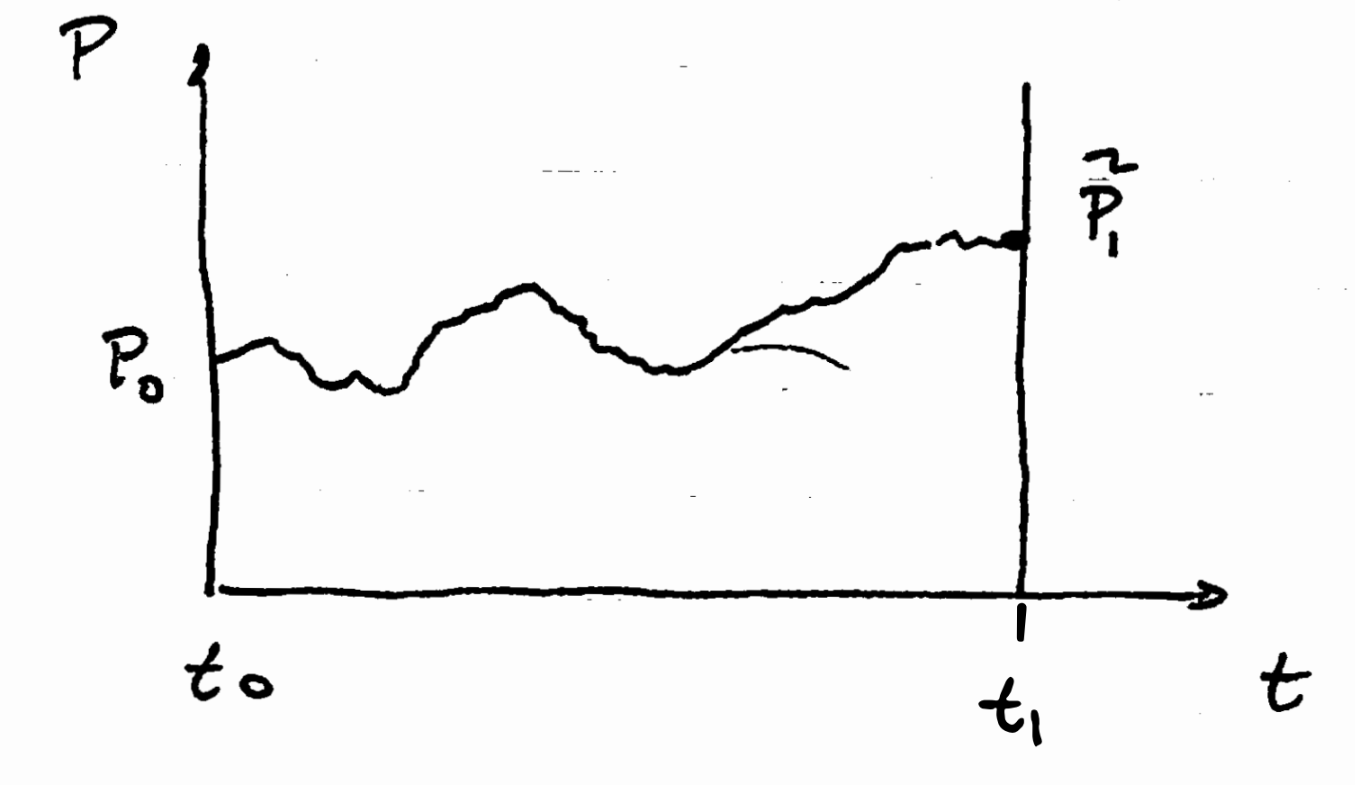
\includegraphics[width=0.4\textwidth]{images/L8-diffusion.png}
    \centering
\end{figure}
\end{frame}

\begin{frame}
Continuous (no jumps), non-differentiable process\\
\begin{figure}[diffusion]
    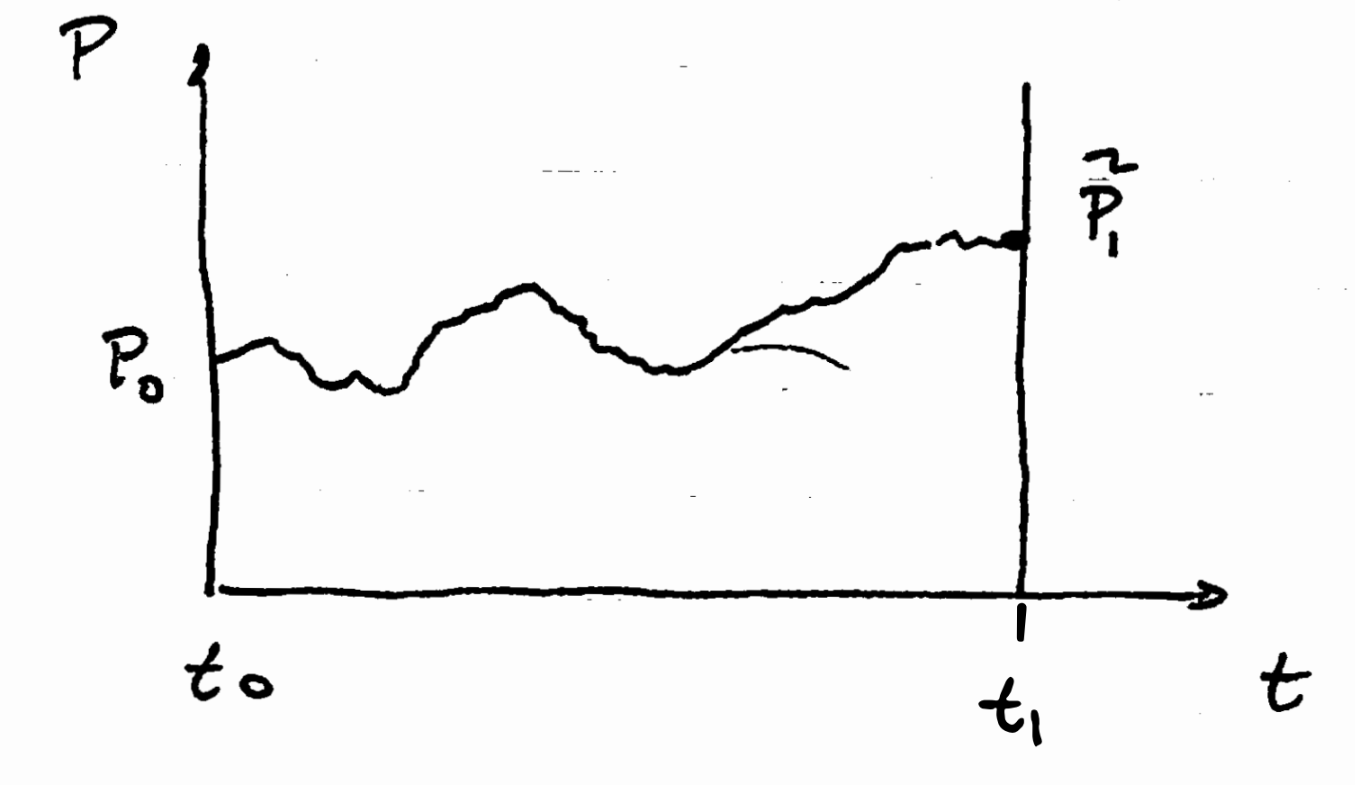
\includegraphics[width=0.6\textwidth]{images/L8-diffusion.png}
    \centering
\end{figure}
We will see if $\mu$ and $\sigma$ are constants, the distribution of $\tilde P_1$ is log-normal.\\
\end{frame}

\begin{frame}
It is generally useful to think of the Wiener process $dv$ as:\\
\begin{figure}[diffusion]
    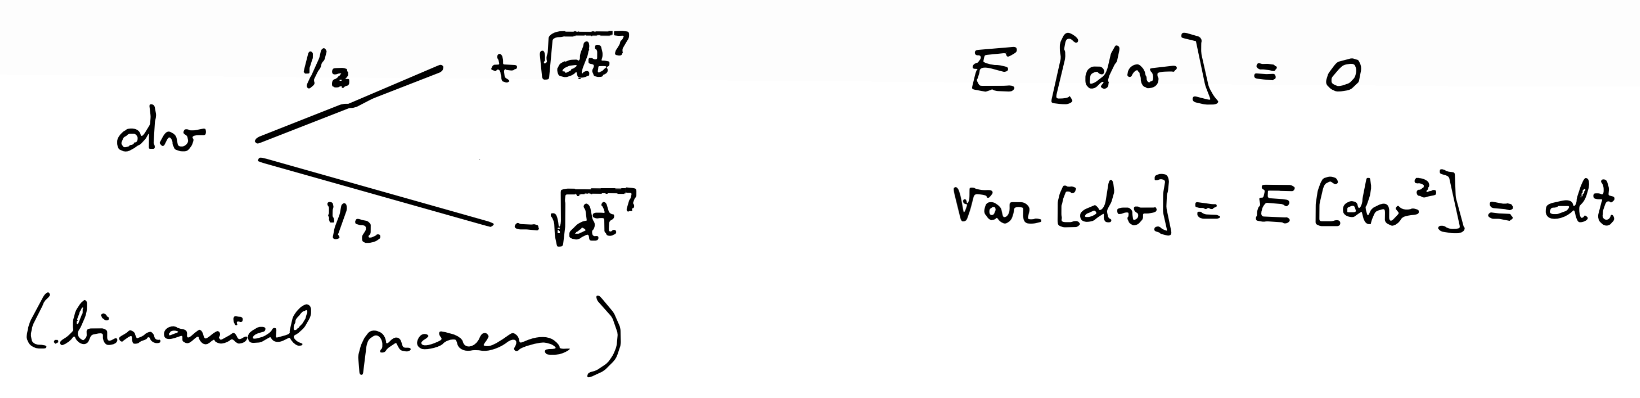
\includegraphics[width=1\textwidth]{images/L8-wiener.png}
    \centering
\end{figure}
Also note that even though $dv$ is stochastic, $dv^2$ is non-stochastic (in probability limit).
\begin{figure}[diffusion]
    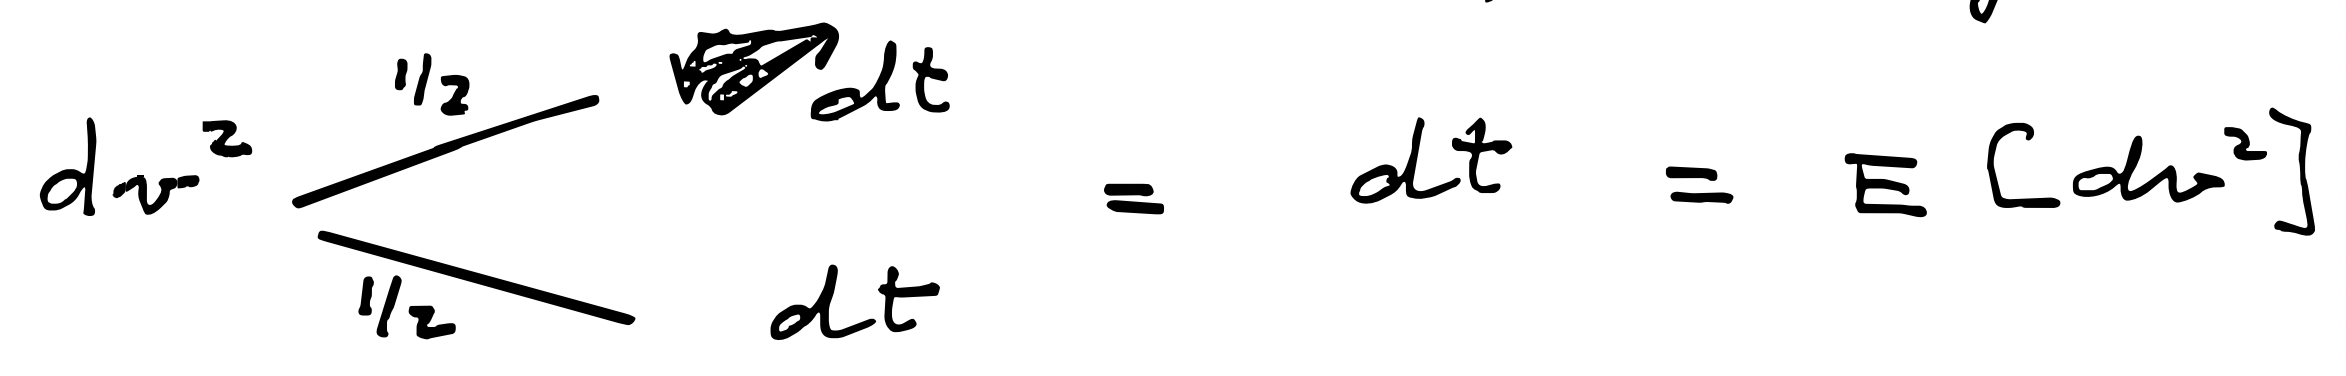
\includegraphics[width=0.8\textwidth]{images/L8-wiener2.png}
    \centering
\end{figure}
\end{frame}

\subsection{Chebyshev's Inequality}
\begin{frame}
If the mean ($\mu$) and variance ($\sigma^2$) of a distribution $\tilde{y}$ exist, then\\
\[Prob[|\tilde y - \mu| \geq \theta] \leq \frac{\sigma^2}{\theta^2}\]
For example, if $\tilde{y} = d\tilde{v}^2 = \tilde x^2 dt$,\\
\begin{align*}
    \longrightarrow E[d\tilde{v}^2] =&\; E[\tilde{x}^2 dt] = dt\\
    E[(d\tilde{v}^2 - dt)^2] =&\; E[d\tilde{v}^4] - dt^2 = E[d\tilde{x}^4 dt^2] - dt^2 = (m_4 - 1)dt^2\\
    \longrightarrow var(d\tilde{v}^2) =&\; 0 (dt^2)\\
\end{align*}
\[\therefore Prob[|\tilde y - \mu| \geq \theta] \leq \frac{(m_4-1)}{\theta^2}dt^2 = 0(dt^2)\]
\[\implies {p\!\!-\!\!\lim}\; d\tilde{v}^2 = dt\]
\end{frame}

\begin{frame}
Also,\\
\begin{align*}
    E[d\tilde{v_i}d\tilde{v_j}] =&\; E[\tilde{x_i}\sqrt{dt}\tilde{x_j}\sqrt{dt}] = \rho dt\\
    E[(d\tilde{v_i}d\tilde{v_j}-\rho dt)^2] =&\; E[\tilde{x_i^2}\tilde{x_j^2}dt^2]-\rho^2 dt^2\\
    =&\; (E[\tilde{x_i^2}\tilde{x_j^2}]-\rho^2) dt^2 = (m_{2,2}-\rho^2)dt^2\\
\end{align*}
\[\therefore Prob[|d\tilde{v_i}d\tilde{v_j} - \rho dt| \geq \theta] \leq \frac{(m_{2,2}-\rho^2)}{\theta^2}dt^2 = 0(dt^2)\]
\[\implies {p\!\!-\!\!\lim}\; d\tilde{v_i}d\tilde{v_j} = \rho dt\]
\end{frame}

% \begin{frame}
% \begin{align*}
%     E[\frac{dP}{P}] =&\; \mu dt + \sigma E[dv]\\
%     =&\; \mu dt + \sigma \cdot 0\\
% \end{align*}
% \[\therefore \mu = \frac{E[\frac{dP}{P}]}{dt} \;\;\;\; \textit{the instantaneous expected rate of return}\]
% \end{frame}

% \begin{frame}
% \begin{align*}
%     (\frac{dP}{P})^2 =&\; \mu^2 dt^2 + 2\mu\sigma \; dt \; dv + \sigma^2 dt^2\\
%     =&\; 0 + 0 + \sigma^2 dt^2\\
% \end{align*}
% \[\therefore \sigma^2 = \frac{(\frac{dP}{P})^2}{dt} = \frac{E[\frac{dP}{P}]^2}{dt} \;\;\;\; \textit{the instantaneous variance of return}\]
% \end{frame}

% \begin{frame}
% Then,\\
% \[\frac{dP}{P} = \mu dt + \sigma dv\]
% The instantaneous return equals the expected return (of magnitude $dt$) plus the unanticipated return (of magnitude $\sqrt{dt}$).
% \end{frame}

% \begin{frame}
% For two assets,\\
% \begin{align*}
%     \frac{dP_i}{P_i} =&\; \mu_i dt + \sigma_i dv_i\\
%     \frac{dP_j}{P_j} =&\; \mu_j dt + \sigma_j dv_j\\
% \end{align*}
% \[\therefore \frac{dP_i}{P_i}\cdot\frac{dP_j}{P_j} = \mu_i\mu_j dt^2 + \mu_i\sigma_j\;dt\;dv_j + \mu_j\sigma_i\;dt\;dv_i + \sigma_i\sigma_j\;dv_i\;dv_j\]
% \end{frame}

% \begin{frame}
% \[\therefore \frac{dP_i}{P_i}\cdot\frac{dP_j}{P_j} = \mu_i\mu_j dt^2 + \mu_i\sigma_j\;dt\;dv_j + \mu_j\sigma_i\;dt\;dv_i + \sigma_i\sigma_j\;dv_i\;dv_j\]
% the first three terms are order $< dt$, so:
% \[\frac{dP_i}{P_i}\cdot\frac{dP_j}{P_j} = 0 + 0 + 0 + \sigma_i\sigma_j\;dv_i\;dv_j\]
% and $dv_i\;dv_j=\rho_{ij}dt$ represents the correlation between $dv_i$ and $dv_j$, so:
% \[\frac{dP_i}{P_i}\cdot\frac{dP_j}{P_j} = \sigma_i\sigma_j\rho_{ij}dt \equiv \sigma_{ij} dt\]
% \end{frame}

\subsection{Ito's Lemma}
\begin{frame}
\textbf{Ito's Lemma}: The rule to compute the total differential in the presence of stochastic variables (diffusion process):
\[F \equiv F(P;t)\]
\[dF = F_P dP + F_t dt + \frac{1}{2} F_{PP}(dP)^2\]
The first two terms are the classical total differential if $P$ and $t$ are deterministic.\\
\hfill\break
If $P$ is stochastic, we have to add the next term in the Taylor series expansion because $(dP)^2$ is of order $dt$.
\end{frame}

\begin{frame}
Therefore if $\frac{dP}{P} = \mu dt + \sigma dv$,\\
\begin{align*}
    dF =&\; F_P(\mu P dt + \sigma P dv)+F_t dt + \frac{1}{2} F_{PP}(\sigma^2 P^2 dt)\\
    dF =&\; (\frac{1}{2} \mu^2P^2 F_{PP}+\mu P F_P+F_t)dt+P F_P \sigma dv\\
\end{align*}
In general, if $F \equiv F(P_1,...,P_n,t)$ then\\
\[dF = \sum_{i=1}^n F_{P_i}dP_i + F_tdt + \frac{1}{2} \sum_{i=1}^n\sum_{j=1}^n F_{P_iP_j}(dP_i)(dP_j)\]
where $(dP_i)(dP_j) = P_i P_j \sigma_{ij} dt$\\
\end{frame}

\begin{frame}
And more generally,
\begin{align*}
    dP =&\; \mu(P,t) dt + \sigma(P,t) dv\\
    (dP)^2 =&\; \sigma^2(P,t) dt\\
\end{align*}
So  Ito's Lemma:
\[dF = F_P dP + (F_t + \frac{1}{2} \sigma^2(P,t)F_{PP})dt\]
\end{frame}

\begin{frame}
\underline{Example}:
\begin{align*}
    \frac{dP}{P} =&\; \alpha dt + \sigma dv\\
    dP =&\; \alpha P dt + \sigma P dv\\
\end{align*}
and let $Y = \ln{P}$ such that
\begin{align*}
    Y_P =&\; \frac{1}{P} \;\;\;\; Y_t=0\\
    Y_{PP} =&\; -\frac{1}{P^2}\\
\end{align*}
\end{frame}

\begin{frame}
\underline{Example}: applying Ito's Lemma
\begin{align*}
    dY =&\; Y_P dP + \frac{1}{2} Y_{PP} (dP)^2\\
    dY =&\; \frac{P}{P}(\alpha dt + \sigma dv)-\frac{1}{2} \frac{P^2}{P^2} \sigma^2 dt\\
    dY =&\; (\alpha - \frac{1}{2}\sigma^2)dt + \sigma dv\\
\end{align*}
$Y$ receives i.i.d. random investments with instantaneous mean $\mu = (\alpha - \frac{1}{2}\sigma^2)$ and instantaneous variance $\sigma^2$.
Therefore, by the Central Limit Theorem, the change in $Y$ over any finite time interval $(0,T)$, $Y_T-Y_0$, is normally distributed with mean $\mu T$ and variance $\sigma^2 T$ (for $\mu$ and $\sigma$ constant).
\end{frame}

\begin{frame}
\underline{Example}: 
\[Y_T - Y_0 = \; \ln{P_T} - \ln{P_0} = \ln{\frac{P_T}{P_0}} = \ln{(1+z_T)}\]
\begin{align*}
    \ln{\frac{P_T}{P_0}} \sim &\; \mathcal{N}(\mu T, \sigma^2 T)\\
    \frac{P_T}{P_0} \sim &\; \mathcal{LN}(\mu T, \sigma^2 T)\\
\end{align*}
it can be shown that:
\[E[\frac{\tilde P_T}{P_0}]=e^{\mu T +\frac{1}{2}\sigma^2T} = e^{\alpha T}\]
\end{frame}

\begin{frame}
\underline{Example}: 
\[E[\frac{\tilde P_T}{P_0}]=e^{\mu T +\frac{1}{2}\sigma^2T} = e^{\alpha T}\]
therefore the instantaneous (continuously compounding) expected rate of return is $\alpha$.
therefore if $\alpha$ and $\sigma$ are constant, price relatives are log-normally distributed.
\begin{figure}[diffusion]
    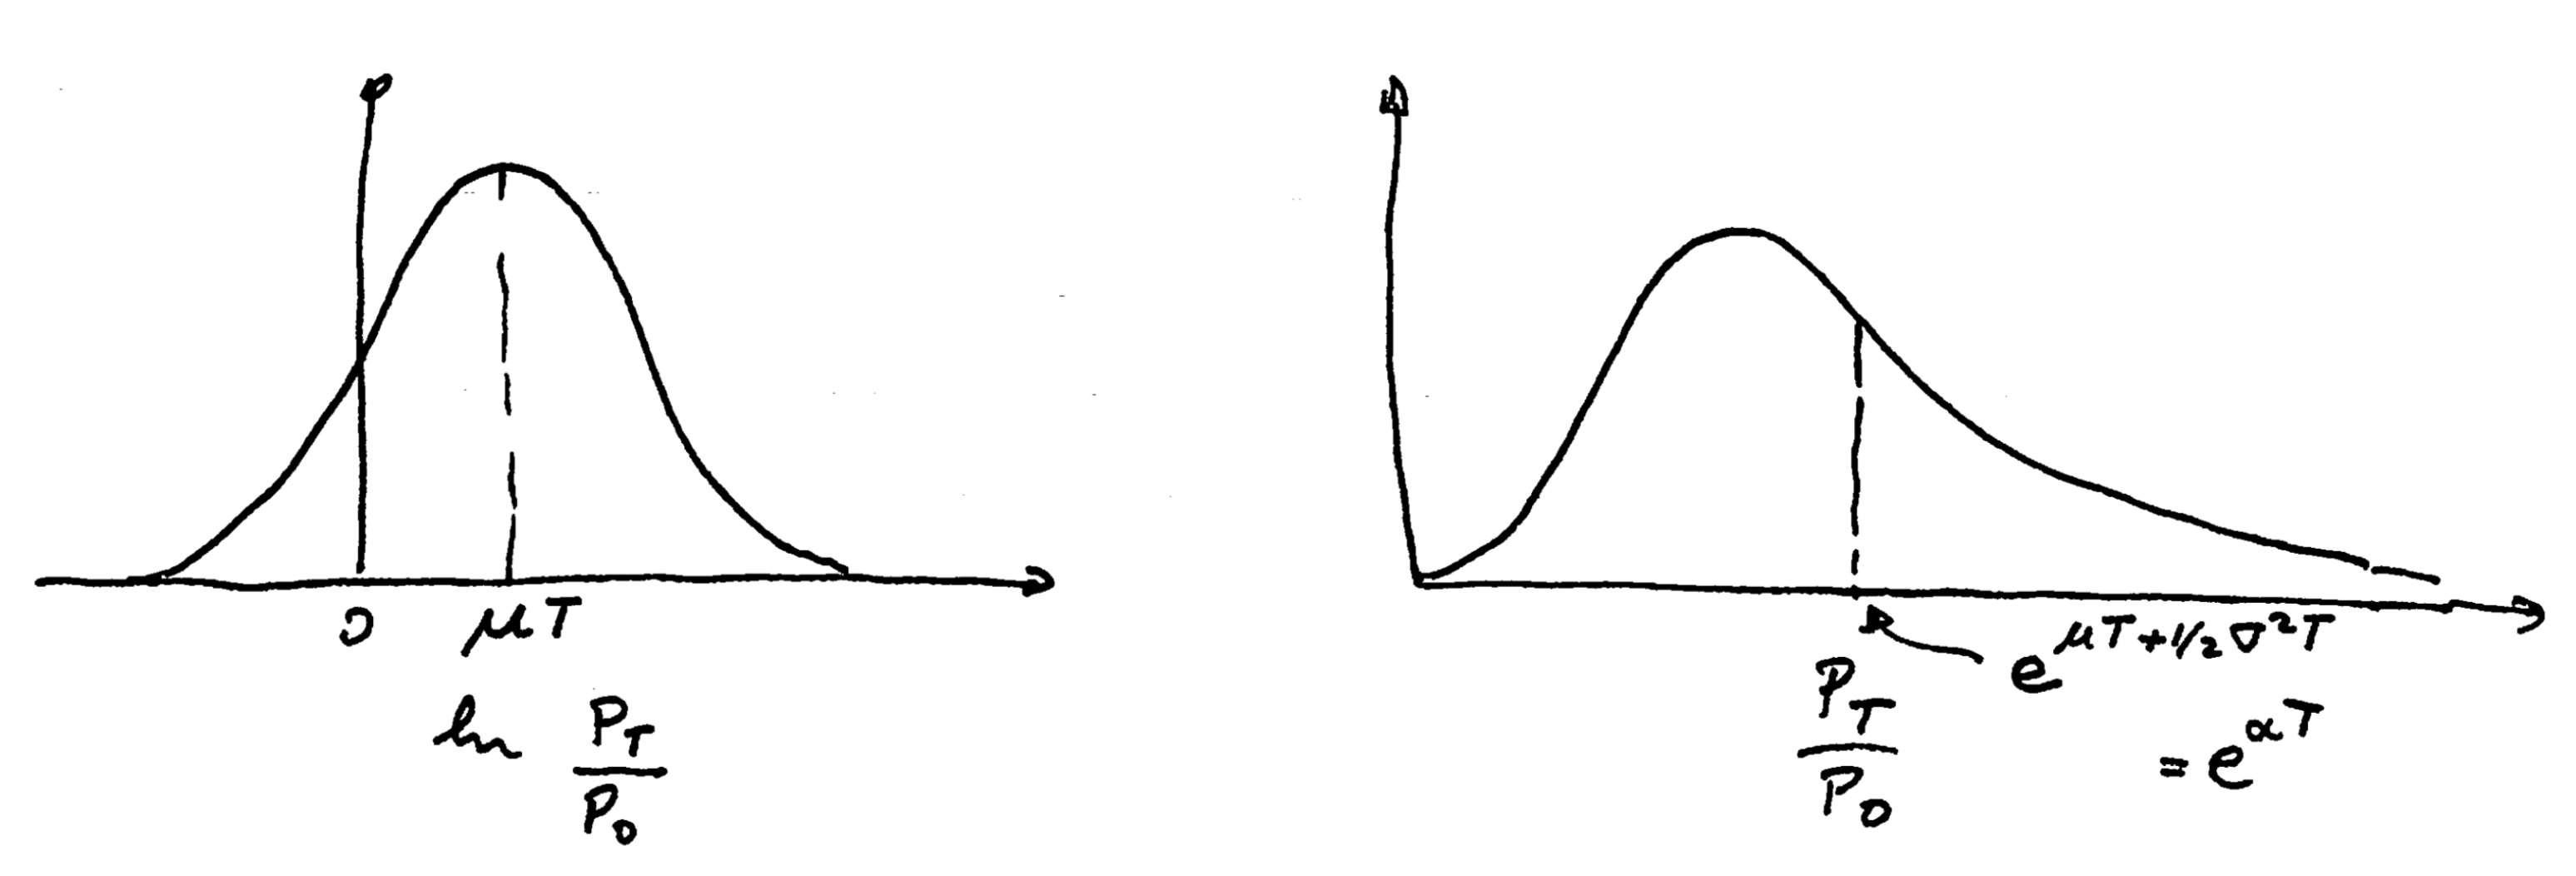
\includegraphics[width=0.9\textwidth]{images/L8-lognormal.png}
    \centering
\end{figure}
\end{frame}

%%%%%%%%%%%%%%%%%%%%%%%%%%%%%%%%%%%%%%%%%%%%%%%%%%%%%%%%%%%%%%%%%%%%%%%%%%%
%%%%%%%%%%%%%% TOPIC 9   %%%%%%%%%%%%%%%
%%%%%%%%%%%%%%%%%%%%%%%%%%%%%%%%%%%%%%%%%%%%%%%%%%%%%%%%%%%%%%%%%%%%%%%%%%%
\section{Continuous Time Portfolio Selection}
\begin{frame}
Suppose that security prices are such that their realized rates of return are compact with means and variances of equal importance, ie. the rate of return $\tilde z(t)$ follows:
\begin{equation}
    \tilde z_i(t) \equiv \frac{dP_i}{P_i} = \alpha_i dt + \sigma_i dv_i
\end{equation}
\begin{align*}
    \textit{with}\;\;\;\; &E[\frac{dP_i}{P_i}] =\; \alpha_i dt\\
    &E[(\frac{dP_i}{P_i})^2] =\; Var[\frac{dP_i}{P_i}] = \sigma_i^2 dt\\
    &E[(\frac{dP_i}{P_i})(\frac{dP_j}{P_j})] =\; \sigma_{ij}^2 dt = \sigma_i \sigma_j \rho_{ij} dt\\
\end{align*}
For the moment we assume that these parameters are constant (for log-normal distribution).\\
\end{frame}

\begin{frame}
The continuous-time version of the portfolio problem (assuming again a time-additive and state-independent utility function of consumption) is:\\
\begin{equation} \tag{2}
    \max_{C(t),\vec{w}(t)} E_0\bigg[\int_0^T U(C,t)dt + B[W(T),T]\bigg]
\end{equation}
The wealth accumulation equation:\\
\begin{equation} \tag{3}
    W(t+dt) = [W(t)+Y(t)dt-C(t)dt] \sum_{i=0}^n w_i(t)(1+z_i(t))
\end{equation}
where $C(t)$ and $Y(t)$ are now flows...
\end{frame}

\begin{frame}
For simplicity, assume $Y=0$,
\begin{align*}
    W(t+dt) &= [W(t)-C(t)dt] \bigg[1 + \sum_{i=0}^n w_i(t)(z_i(t)) \bigg] \;\;\Bigg\} \bigg[1 + \sum_{i=0}^n w_i(\frac{dP_i}{P_i}) \bigg]\\
    &= W(t)-C(t)dt+W(t)\sum_{i=0}^n w_i\frac{dP_i}{P_i}\\
    \therefore \;\; dW(t) &= -C(t)dt + W(t)\sum_{i=0}^n w_i\frac{dP_i}{P_i}\\
    &\textit{but} \;\;\;\; \sum_{i=0}^n w_i\frac{dP_i}{P_i} = \sum_{i=1}^n w_i[\alpha_i dt + \sigma_i dv_i] + \bigg(1-\sum_{i=1}^n w_i\bigg)r dt\\
    &\;\;\;\;\;\;\;\;\;\;\;\;\;\;\;\;\;\;\;\;\;\;\;\;\;\; = \bigg\{\sum_{i=1}^n w_i(\alpha_i-r) + r \bigg\}dt + \sum_{i=1}^n w_i \sigma_i dv_i \;\;\;\; \textit{...}\\
\end{align*}
\end{frame}

\begin{frame}
So,
\begin{equation} \tag{4}
    dW(t) = -C(t)dt + W(t)\Bigg[\sum_{i=1}^n w_i(\alpha_i-r) + r\Bigg]dt +W(t)\sum_{i=1}^n w_i \sigma_i dv_i
\end{equation}
and,
\begin{align} \tag{5}
\begin{split}
    E_t[dW(t)] &= -Cdt + W\Bigg[\sum w_i(\alpha_i-r) + r\Bigg]dt = \alpha_w dt
    \\
    Var_t[dW] &= E_t[dW^2] = W^2 \sum_{i=1}^n \sum_{j=1}^n w_i w_j \sigma_{ij} dt = \sigma_w^2 dt 
\end{split}
\end{align}
where the summations can be replaced with their vector equivalents...
\end{frame}

\begin{frame}
where the summations can be replaced with their vector equivalents...
\begin{align} \tag{5'}
\begin{split}
    E_t[dW(t)] &= -Cdt + W\bigg[\vec{w}'(\vec\alpha-r\vec1)+r\bigg]dt = \alpha_w dt
    \\
    Var_t[dW] &= E_t[dW^2] = W^2 \bigg[ \vec{w}'\bm{\Sigma}\vec{w}\bigg] dt = \sigma_w^2 dt 
\end{split}
\end{align}
and,
\begin{align*}
    dW &= \alpha_w dt + \sigma_w dv_w\\
    \sigma_w dv_w &= W \sum w_i \sigma_i dv_i\\
\end{align*}
\end{frame}

\begin{frame}
Define again the derive utility function of wealth,
\begin{equation} \tag{6}
    J[W(t),t] \equiv \max E_t \Bigg[ \int_t^T U(C,S)dS + B[W(T),T] \Bigg]
\end{equation}
Then,
\begin{equation} \tag{7}
    J[W(t),t] = \max E_t \Bigg[ \int_t^{t+dt} U(C,S)dS + J[W(t+dt),t+dt] \Bigg]
\end{equation}
\[\textit{but:}\;\;\;\; \int_t^{t+dt} U(C,S)dS = U(C,t)dt\]
and applying Ito's Lemma,
\[ J[W(t+dt),t+dt] = J[W,t] + J_tdt + J_WdW + \frac{1}{2} J_{WW}(dW)^2\]
\end{frame}

\begin{frame}
Substituting in (7), taking $E_t$, substituting (5), eliminating $J$ from both sides of the equation, and finally dividing by $dt$...\\
\begin{align*}
    \frac{dP_i}{P_i} &= \alpha_i dt + \sigma_i dv_i\\
    dW &= -C dt + W\sum_{i=0}^n w_i \frac{dP_i}{P_i}\\
    E_t[dW] &= -C dt + W \sum_{i=0}^n w_i\alpha_i dt = -C dt + W \vec{w}'\vec{\alpha} dt\\
    E_t[dW^2] &= W^2 \sum_{i=1}^n \sum_{i=1}^n w_i w_j \sigma_{ij} dt = -W^2 \vec{w}'\bm{\Sigma}\vec{w} dt\\
\end{align*}
\end{frame}

\begin{frame}
We obtain
\begin{align*}
    J[W(t),t] &\equiv \max\;E_t \Bigg[ \int_t^T U(C,S)dS + B[W(T),T]\\
    &= \max E_t \Bigg[U(C,t)dt + J[W(t+dt),t+dt)]\Bigg]\\
\end{align*}
or, \textbf{(8)} Bellman Equation: Stochastic Control Theory\\
\begin{align*}
    0 &= \max_{C,\vec{w}} \Bigg\{ U(C,t)+J_t+J_W[-C+W(\sum_{i=1}^n w_i(\alpha_i-r)+r)] + \frac{W^2}{2} J_{WW} \sum_{i=1}^n \sum_{j=1}^n w_i w_j \sigma_{ij} \Bigg\}\\
    0 &= \max_{C,\vec{w}} \Bigg\{ U(C,t)+J_t+J_W[-C+W(\vec{w}'(\vec{\alpha}_i-\vec{1}r)+r)] + \frac{W^2}{2} J_{WW} \vec{w}' \bm{\Sigma} \vec{w} \Bigg\}\\
\end{align*}
\end{frame}

\begin{frame}
\underline{1st order conditions:}\\
\begin{equation} \tag{9a}
    U_C = J_W \;\;\;\; \textit{envelope condition}
\end{equation}
\begin{equation} \tag{9b}
    J_W \cdot W(\vec{\alpha}-r\vec{1}) + J_{WW} W^2 \bm{\Sigma} \vec{w} = 0
\end{equation}
a set of linear equations, the same we get in mean-variance analysis.\\
\begin{equation} \tag{10}
    \vec{w}^* = -\frac{J_W}{W J_{WW}} \bm{\Sigma}^{-1}(\vec{\alpha} - r\vec{1})
\end{equation}
therefore $\frac{w_i^*}{w_j^*}$ is independent of utility.\\
$\longrightarrow$ two fund separation $\longrightarrow$ all investors hold the same risky portfolio $\longrightarrow$ the market.\\
\[\vec{m} = \frac{\bm{\Sigma}^{-1}(\vec{\alpha}-r\vec{1})}{\vec{1} \bm{\Sigma}^{-1}(\vec{\alpha}-r\vec{1})}\]
\end{frame}

\begin{frame}
Equilibrium can be obtained from (9b)
\[ \Bigg(-\frac{J_W^k}{J_{WW}^k}\Bigg)(\vec{\alpha} - r\vec{1}) = W^k \bm{\Sigma} \vec{w}^k \]
risk tolerance//
\hfill\break
Summing over all investors: $\sigma_k$, in equilibrium demand = supply for each firm.\\
\[ A (\vec{\alpha} - r\vec{1}) = \bm{\Sigma}\vec{V} \]
\end{frame}

\begin{frame}
\[ A (\vec{\alpha} - r\vec{1}) = \bm{\Sigma}\vec{V} \]
where
\[ A = \Sigma_k \Bigg(-\frac{J_W^k}{J_{WW}^k}\Bigg) \]
\[ \vec{V} = \Sigma_k W^k \vec{w}^k = \;\;\textit{value of firms} \]
\[ \vec{m} = \frac{\vec{V}}{\vec{1}\vec{V}} = \frac{\vec{V}}{M} \;\;\;\;\therefore\;\;\;\; \vec{V} = M\vec{m}\]
\[ \therefore \;\; A(\vec{\alpha}-r\vec{1}) = M \bm{\Sigma}\vec{m}\]
\hfill\break
where $\bm{\Sigma}\vec{m}$ represent covariances with the market...\\
\end{frame}

\begin{frame}
Pre-multiplying by $\vec{m}'$\\
\[ A(\alpha_m-r) = M \sigma_m^2 \]
\begin{equation} \tag{11}
    \therefore \;\; \alpha_i-r = \frac{\sigma_{im}}{\sigma_m^2}(\sigma_m-r) = \beta_i (\alpha_m -r)
\end{equation}
\hfill\break
ie. the CAPM holds for continuously compounded rates of return (\textit{Merton's ICAPM}) for a broad class of utility functions, compact distributions.
\end{frame}

\begin{frame}
If \underline{all} investors have \underline{log utility functions} (we will show later that if $U$ is log, $J$ is also logarithmic)\\
\begin{align*}
    -\frac{J_W^k}{J_{WW}^k W^k} &= 1\;\;\;\;\textit{relative risk aversion}\\
    -\frac{J_W^k}{J_{WW}^k} &= W^k\\
\end{align*}
and
\begin{align*}
    A &= \sum_k-\frac{J_W^k}{J_{WW}^k} = W\;\;\;\;\textit{aggregate wealth}\\
    W &= M + \;\textit{net supply of the riskless asset}\\
\end{align*}
\end{frame}

\begin{frame}
\begin{align*}
    \therefore \;\; \vec{\alpha}-r\vec{1} &= \frac{M}{W}\; \bm{\Sigma}\vec{m}\\
    \vec{\alpha}_i-r &= \frac{M}{W}\; \sigma_{im} = \sigma_{iw} \;\;\;\; \textit{covariance with aggregate wealth}\\
\end{align*}
valid only for \underline{log utility}.\\
\hfill\break
If no riskless asset exists then $r$ in (11) is replaced by the expected return on a zero beta portfolio.\\
\begin{equation} \tag{11'}
    \alpha_i-\alpha_0 = \beta_i (\alpha_m-\alpha_0)
\end{equation}
\end{frame}

%%%%%%%%%%%%%%%%%%%%%%%%%%%%%%%%%%%%%%%%%%%%%%%%%%%%%%%%%%%%%%%%%%%%%%%%%%%
%%%%%%%%%%%%%% TOPIC 10   %%%%%%%%%%%%%%%
%%%%%%%%%%%%%%%%%%%%%%%%%%%%%%%%%%%%%%%%%%%%%%%%%%%%%%%%%%%%%%%%%%%%%%%%%%%
\section{Continuous Time Portfolio Selection and Asset Pricing}
\subsection{Review}
\begin{frame}
\begin{align*}
    \frac{dP_i}{P_i} =&\; \alpha_i dt + \sigma_i dv_i\\
    \sigma_{ij} =&\; \bm{\Sigma} \;\;\;\; \textit{Constant opportunity set}\\
\end{align*}
Wealth accumulation equation\\
\begin{align*}
    dW &= \alpha_w dt + \sigma_w dv_w\\
    \alpha_w &= -C + W(\vec{w}'(\vec{\alpha}-r\vec{1})+r)\\
    \sigma_w^2 &= W^2 \vec{w}'\bm{\Sigma}\vec{w}\\
    \sigma_w dv_w &= W \sum_{i=1}^n w_i \sigma_i dv_i
\end{align*}
\end{frame}

\begin{frame}
Time additive utility function:\\
\[ \max_{C(t),\vec{w}(t)}\; E_0\Bigg[\int_0^T U(C,t)dt + B[W(T),T]\Bigg]\]
Derived utility of wealth:\\
\begin{align*}
    J[W(t),t] &\equiv \max\;E_t \Bigg[ \int_t^T U(C,S)dS + B[W(T),T]\\
    &= \max\; E_t \Bigg[U(C,t)dt + J[W(t+dt),t+dt)]\Bigg]\\
\end{align*}
\end{frame}

\begin{frame}
Bellman Equation:
\[ 0 = \max_{C(t),\vec{w}(t)} \Bigg\{ U(C,t)+J_t+J_W[-C+W(\vec{w}'(\vec{\alpha}_i-\vec{1}r)+r)] + \frac{W^2}{2} J_{WW} \vec{w}' \bm{\Sigma} \vec{w} \Bigg\} \]
First Order Conditions:
\begin{align*}
    U_C &= J_W\\
    \vec{w}^* &= -\frac{J_W}{W J_{WW}}\;\bm{\Sigma}^{-1}(\vec{\alpha}-r\vec{1})
\end{align*}
\underline{Implies}: Two-fund separation, ICAPM (Merton)\\
If we know $U(\cdot)$ we can solve for $C(\cdot)$ and $\vec{w}(\cdot)$ as a function of $J_W$, $J_{WW}$, etc... and substitute in the Bellman equation $\implies$ PDE for $J$.\\
\end{frame}

\subsection{Example}
\begin{frame}
Power utility $U(C,t) = e^{-\rho t}\frac{C^\gamma}{\gamma}$, no motive for bequest.\\
\hfill\break
Since we will always hold the market, we can assume that it is the only risky asset.\\
\hfill\break
From (8),
\begin{equation} \tag{12}
    0 = \max \Bigg[ e^{-\rho t}\frac{C^\gamma}{\gamma} + J_t + J_W[W(w(\alpha-r)+r)-C] + \frac{w^2W^2}{2}\sigma^2 J_{WW} \Bigg]
\end{equation}
\end{frame}

\begin{frame}
The optimal $C^*$ and $w^*$ are from (9a) and (10)\\
\[ e^{-\rho t}{C^*}^{\gamma-1} = J_W \;\;\implies\;\; C^* = (e^{\rho t}J_W)^{\frac{1}{\gamma-1}}\]
\[ w^* = \bigg(-\frac{J_W}{W J_{WW}}\bigg) \frac{\alpha-r}{\sigma^2} \]
Substituting in (12), we get a PDE for J:
\begin{align*}
\begin{split}
    0 = \frac{e^{-\rho t}}{\gamma} \bigg(e^{\rho t}J_W\bigg)^{\frac{\gamma}{\gamma-1}} + J_t + J_W\Bigg[ W\bigg[-\frac{J_W}{W J_{WW}}\frac{(\alpha-r)^2}{\sigma^2}+r\bigg] - (e^{\rho t}J_W)^{\frac{1}{\gamma-1}} \Bigg]&
    \\
    + \frac{1}{2}\frac{J_W^2}{J_{WW}} \frac{(\alpha-r)^2}{\sigma^2}&
\end{split}
\end{align*}
\end{frame}

\begin{frame}
\begin{equation} \tag{13}
    0 = e^{-\rho t} \bigg(\frac{1}{\gamma}-1\bigg)\bigg(e^{\rho t}J_W\bigg)^{\frac{\gamma}{\gamma-1}} + J_t + rWJ_W-\frac{1}{2}\frac{(\alpha-r)^2}{\sigma^2}\frac{J_W^2}{J_{WW}}
\end{equation}
with boundary condition: $J(W(T),T)=0$.\\
\hfill\break
Difficult PDE. Consider the $\infty$ horizon problem and for this problem try:\\
\[ J(W,t) = e^{-\rho t}I(W)\]
Then $J_t = -\rho I e^{-\rho t}$, $J_W = e^{-\rho t} I'$, $J_{WW} = e^{-\rho t} I''$...
\end{frame}

\begin{frame}
By substitution in (13) we obtain the PDE (dividing by $e^{-\rho t}$):
\[ 0 = \bigg(\frac{1-\gamma}{\gamma}\bigg)(I')^{\frac{\gamma}{\gamma-1}} - \rho I + rW I' - \frac{1}{2}\frac{(\alpha-r)^2}{\sigma^2}\frac{(I')^2}{I''}\]
Guess a solution of the form $I(W) = \frac{AW^\gamma}{\gamma}$. Substitution leaves\\
\[ 0 = AW^\gamma \bigg[ \frac{1-\gamma}{\gamma}A^{\frac{1}{\gamma-1}} - \frac{\rho}{\gamma}+r-\frac{1}{2}\bigg(\frac{(\alpha-r}{\sigma}\bigg)^2\frac{1}{\gamma-1}\bigg]\]
verifying this solution form for the constant:\\
\[ A = \Bigg[ \frac{\gamma}{1-\gamma} \bigg[ \frac{\rho}{\gamma} -r - \frac{1}{2}\bigg(\frac{\alpha-r}{\sigma}\bigg)^2\frac{1}{1-\gamma}\bigg]\Bigg]^{\gamma-1} \equiv a^{\gamma-1} \]
\end{frame}

\begin{frame}
\[ A = \Bigg[ \frac{\gamma}{1-\gamma} \bigg[ \frac{\rho}{\gamma} -r - \frac{1}{2}\bigg(\frac{\alpha-r}{\sigma}\bigg)^2\frac{1}{1-\gamma}\bigg]\Bigg]^{\gamma-1} \equiv a^{\gamma-1} \]
\[ \therefore \;\;\;\; J = e^{-\rho t} a^{\gamma-1} \frac{W^\gamma}{\gamma}\]
and the optimal choices
\begin{align*}
    C^* &= a\;W\\
    w^* &= \frac{\alpha-r}{(1-\gamma)\sigma^2}
\end{align*}
are independent of calendar time.
\end{frame}

\begin{frame}
For the finite horizon case, guess the solution:\\
\[ J(W,t) = e^{-\rho t} B(t) \cdot A \frac{W^\gamma}{\gamma}\]
Substitution into (13) verifies the guess where $B(t)$ is the solution to the 1st order ODE:\\
\[ B'(t) = (1-\gamma) \bigg[ aB-B^{\frac{-\gamma}{1-\gamma}}\bigg]\]
with boundary condition $B(T)=0$.\\
\end{frame}

\begin{frame}
Solution,\\
\[ B(t) = \bigg[ 1-e^{a(t-T)}\bigg]^{1-\gamma}\]
with optimal choices:\\
\begin{align*}
    C^* &= \frac{a}{1-e^{a(t-T)}}W(t)\;\;\;\; \textit{dep. on return characteristics (except in log case)}\\
    w^* &= \frac{\alpha-r}{(1-\gamma)\sigma^2}\;\;\;\;\;\;\;\;\;\;\;\textit{indep. of W, C, and $\rho$}
\end{align*}
\end{frame}

\subsection{Solution Procedure}
\begin{frame}
\underline{Solution steps} for equation (13)\\
\begin{enumerate}
    \item Consider first the $\infty$ horizon problem.
    \item Try separation of variables (eg. $J(W,t) = e^{-\rho t} I(W)$) such that we obtain a second order ODE for $I(W)$.
    \item Try solution $I(W) = A \frac{W^\gamma}{\gamma}$. It works and we compute $A$.
    \item Solution to $\infty$ horizon case (eg. $J = e^{-\rho t} A \frac{W^\gamma}{\gamma}$).
    \item For finite horizon, guess solution $J = A \frac{W^\gamma}{\gamma}\cdot B(t) \cdot A\frac{W^\gamma}{\gamma}$.
    \item Substitute into original equation, this gives an ODE for $B(t)$.
\end{enumerate}
\end{frame}

%%%%%%%%%%%%%%%%%%%%%%%%%%%%%%%%%%%%%%%%%%%%%%%%%%%%%%%%%%%%%%%%%%%%%%%%%%%
%%%%%%%%%%%%%% TOPIC 11   %%%%%%%%%%%%%%%
%%%%%%%%%%%%%%%%%%%%%%%%%%%%%%%%%%%%%%%%%%%%%%%%%%%%%%%%%%%%%%%%%%%%%%%%%%%
\section{Extended Model}

\subsection{Introduction to the Extended Model}

\begin{frame}
In equilibrium, weights of the market portfolio,\\
\[ \vec{m} = \frac{\bm{\Sigma}^{-1}(\vec{\alpha}-r\vec{1})}{\vec{1}'\bm{\Sigma}^{-1}(\vec{\alpha}-r\vec{1})} \]
and all investors hold this portfolio (and the riskless asset).\\
\hfill\break
But, if the investment opportunity set remains constant, then $\vec{m}$ is constant, which implies that the realized returns on all assets are constant! (apart from supply adjustments)\\
\hfill\break
This problem exists only in the ICAPM, since in the single period CAPM we only had one return.
\end{frame}

\begin{frame}
\underline{Extension of the Model}\\
\hfill\break
Strong Result $\longrightarrow$ CAPM holds for continuously compounded rates of return if prices have continuous sample paths.\\
\hfill\break
However, we assume that an investor can measure their well-being at any point in time by knowing only their wealth - ie. in (6) we assumed that $J(\cdot)$ is independent of the "state of the world".\\
\hfill\break
If relative commodity prices change, then utilities of consumption will be state dependent and so will $J$. Even if utility is state independent, there may be individual dependencies in the $J$ function if $\alpha$, $\sigma$, and $r$ vary randomly over time.
\end{frame}

\begin{frame}
Suppose there is a simple state variable which describes changes in these variables, $\alpha_i(x)$, $\sigma_{ij}(x)$, $r(x)$, and that changes in this state variable follows:\\
\[ dx = \mu dt + s dy \]
\[\textit{with}\;\; (dx)\bigg(\frac{dP_i}{P_i}\bigg) = cov_t\bigg(dx,\frac{dP_i}{P_i}\bigg) = \rho_{ix} s \sigma_i dt = \sigma_{ix} dt\]
As before, applying Ito's Lemma:\\
\begin{align*}
    J[W+dW, x+dx, t+dt] = J(W,x,t)+J_t\;dt &+ J_W\;dW + J_x\;dx + \frac{1}{2}\;J_{WW}\;(dW)^2\\
    &+ \frac{1}{2}\;J_{xx}\;dx^2+J_{xW}\;dx\;dW
\end{align*}
Taking expectations and multiplying as before...
\end{frame}

\begin{frame}
...we end up with\\
\[ \frac{dP_i}{P_i} = \alpha_i dt + \sigma_i dv_i \]
\[ (\sigma_{ij}) = \bm{\Sigma} \]
\[ dx = \mu\;dt + s\;dy \]
\[ (\sigma_{ix}) = \vec{\sigma} \]
\[ dW = \alpha_w dt + \sigma_w dv_w\]
\[ \alpha_w = -C+W(\vec{w}'(\vec{\alpha}-r\vec{1})+r)\]
\[ \sigma_w^2 = W^2\vec{w}' \bm{\Sigma} \vec{w} \]
\[ \sigma_w dv_w = W \sum_i w_i \sigma_i dv_i \]
\[ (dW)(dx) = W\vec{w}'\vec{\sigma} dt \;\; \textit{...}\]
\end{frame}

\begin{frame}
...and\\
\[ J \equiv J(W,x,t) \]
\[ J(W,x,t) = \max_{C(t),\vec{w}(t)}\; E_t \bigg[ U(C,t)dt+J(W+dW,x+dx,t+dt)\bigg]\]
so...
\end{frame}

\begin{frame}
\begin{align} \tag{14}
\begin{split}
    0 = \max_{C,\vec{w}}\; \bigg[ U(C,t)+J_t+&J_W(-C+W\sum_0^n w_i\sigma_i) + \frac{W^2}{2}\;J_{WW}\;\sum_{i=1}^n\sum_{j=1}^n\;w_iw_j\sigma_{ij}
    \\
    &+ J_x\;\mu + \frac{1}{2}\;J_{xx}\;s^2 +J_{xW}\;W\;\sum_1^n\;w_i\sigma_{ix}\bigg]
\end{split}
\end{align}
As before $U_C=J_W$, but now the portfolio weights satisfy
\begin{equation} \tag{15}
    J_W\;W\;(\alpha_i-r)+J_{WW}\;W^2\;\sum_{j=1}^n w_j^* \sigma_{ij} + J_{Wx}\;W\;\sigma_{ix} = 0 \;\; \textit{i=1,...,n}
\end{equation}
Or, in matrix form...
\begin{equation} \tag{15'}
    J_W\;(\vec\alpha-r\vec1)+J_{WW}\;W\;\bm{\Sigma}\vec{w}^* + J_{Wx}\;\vec\sigma = 0
\end{equation}
\end{frame}

\begin{frame}
Or, in matrix form...
\begin{equation} \tag{15'}
    J_W\;(\vec\alpha-r\vec1)+J_{WW}\;W\;\bm{\Sigma}\vec{w}^* + J_{Wx}\;\vec\sigma = 0
\end{equation}
Where $\bm{\Sigma}$ is the covariance matrix of returns and $\vec{\sigma}' = (\sigma_{1x},...,\sigma_{nx})$. Then,
\begin{align} \tag{16}
\begin{split}
    \vec{w}^* &= -\frac{J_W}{W J_{WW}} \bm{\Sigma}^{-1}(\vec\alpha-r\vec1) -\frac{J_{xW}}{W J_{WW}} \bm{\Sigma}^{-1}\vec\sigma
    \\
    w_i^* &= -\frac{J_W}{W J_{WW}} \sum_{j=1}^n v_{ij}(\alpha_j-r) -\frac{J_{xW}}{W J_{WW}} \sum_{j=1}^n v_{ij} \sigma_{jx}
\end{split}
\end{align}
If $x$ changes in a deterministic fashion or is uncorrelated with the returns on all assets, then as before $\frac{w_i^*}{w_j^*}$ is independent of preferences and all investors hold the market.\\
\end{frame}

\begin{frame}
In general, $\frac{w_i^*}{w_j^*}$ is not independent of preferences;\\
however, if we define\\
\[ D \equiv -\frac{J_W}{W J_{WW}} \vec{1}' \bm{\Sigma}^{-1} (\vec\alpha-r\vec1) \;\;,\;\;
    H \equiv -\frac{J_{xW}}{W J_{WW}} \vec{1}' \bm{\Sigma}^{-1} \vec\sigma
\]
then we may write (16) as
\[ w_i^* = D\; \frac{\sum_{j=1}^n v_{ij}(\alpha_j-r)}{\vec1' \bm{\Sigma}^{-1}(\vec\alpha-r\vec1)} + H\; \frac{\sum_{j=1}^n v_{ij} \sigma_{jx}}{\vec1' \bm{\Sigma}^{-1}\vec\sigma}\]
or
\begin{align} \tag{17}
\begin{split}
    w_i^* &= D\;d_i + H\;h_i
    \\
    \vec{w}^* &=  D\;\vec{d} + H\;\vec{h}   
\end{split}
\end{align}
\end{frame}

\begin{frame}
\begin{align} \tag{17}
\begin{split}
    w_i^* &= D\;d_i + H\;h_i
    \\
    \vec{w}^* &=  D\;\vec{d} + H\;\vec{h}   
\end{split}
\end{align}
where $\vec{d} = \bigg( \bm{\Sigma}^{-1}(\vec\alpha-r\vec1)\;/\;\vec1' \bm{\Sigma}^{-1}(\vec\alpha-r\vec1) \bigg)$\;\;,\;\; $\vec{h} = \bigg( \bm{\Sigma}^{-1}\vec\sigma \;/\; \vec1'\bm{\Sigma}^{-1}\vec\sigma \bigg)$\\
\hfill\break
for $\alpha_i$, $h_i$ independent of individual preferences and $\sum d_i = \sum h_i = 1$\\
\hfill\break
$\therefore$ All individuals form their portfolios by buying "shares" in two "mutual funds" $\vec{d}$ and $\vec{h}$. Note that these two portfolios \underline{do not} include the riskless asset.
\end{frame}

\begin{frame}
Portfolio $\vec{d}$ is similar to the single portfolio in the previous problem and, as before, is used to diversify. The second portfolio, $\vec{h}$, is a "hedge" portfolio.\\
\hfill\break
The correlation of portfolio $\vec{h}$ with the state variable $x$ can be obtained from\\
\begin{align*}
    \frac{dY_h}{Y_h} &= \sum h_i \sigma_i\;dt + \sum h_i\sigma_i\;dv_i\\
    dx &= \mu\;dt + s\;dy
\end{align*}
\hfill\break
covariance between return on $\vec{h}$ and change in state variable $x$:
\[ \bigg( \frac{dY_h}{Y_h} \bigg) (dx) = \vec{h}'\vec\sigma\;dt \]
\end{frame}

\begin{frame}
\begin{equation} \tag{18}
    \therefore \;\; \rho_{xh} \equiv \frac{\vec{h}'\vec\sigma}{(\vec{h}'\bm{\Sigma}\vec{h})^{1/2}\cdot s} \;\;\;\; \textit{correlation}
\end{equation}
This is the maximum correlation possible with this set of assets. To see this, take any portfolio $\vec{w}$:\\
\begin{align*}
    \rho_{xw} &= \frac{\vec{w}'\vec\sigma}{(\vec{w}'\bm{\Sigma}\vec{w})^{1/2}\cdot s}\\
    \frac{\partial \rho_{xw}}{\partial \vec{w}} &= \frac{s(\vec{w}'\bm{\Sigma}\vec{w})^{1/2}\vec\sigma-s(\vec{w}'\vec\sigma)\bm{\Sigma}\vec{w}(\vec{w}'\bm{\Sigma}\vec{w})^{-1/2}}{s^2(\vec{w}'\bm{\Sigma}\vec{w})}
\end{align*}
and choose $\vec{w} = \bm{\Sigma}^{-1}\vec\sigma = \vec{h}(\vec1'\bm{\Sigma}^{-1}\vec \sigma)$
\end{frame}

\subsection{Interpretation of portfolios $\vec{d}$ and $\vec{h}$}
\begin{frame}
We will show that $\vec{d}$ above minimizes the variance of changes in \underline{wealth} whereas $\vec{d}$ and $\vec{h}$ together minimize the variance of changes in \underline{consumption}.\\
\hfill\break
Consider the following problems: (1) minimizing the variance of the growth in wealth and consumption subject to consuming $C^*$, (2) earning an expected rate of return on the portfolio equal to that on the portfolio optimally chosen.\\
\[ \eta^* = \vec{w'}^{*} (\vec{\alpha}-r\vec{1})+r \]
For the first problem.\\
\[ \min \;\sigma_W^2 \;\;\textit{s.t.}\;\; \eta=\eta^* \]
\end{frame}

\begin{frame}
\begin{align*}
    L &= \sigma_W^2 + \lambda(\eta^* - \eta)\\
    \frac{\partial L}{\partial \vec{w}} &= 2W^2\bm{\Sigma}\vec{w} - \lambda(\vec\alpha-r\vec1) = 0
\end{align*}
\[ \vec{w}^{**} = \frac{\lambda}{2W^2}\;\bm{\Sigma}^{-1}(\vec\alpha-r\vec1 )\]
Normalizing the sum of these weights to units gives:\\
\[ \vec{w}^{**} = \vec{d} \]
Thus $\vec{d}$ alone would represent the best risk-return trade-off if wealth were the proper criterion for judging...
\end{frame}

\begin{frame}
But utility comes only indirectly from wealth:\\
\hfill\break
Optimal consumption depends upon wealth, age, and state of the world.
\[ C \equiv C(W,x,t) \;\;\;\; \textit{optimal $C^*$}\]
\begin{align*}
    dC &= C_W\;dW + C_x\;dx+C_t\;dt + \frac{1}{2}\;C_{WW}\;(dW)^2 + C_{Wx}\;dx\;dW + \frac{1}{2}\;C_{xx}\;(dx)^2
\end{align*}
or
\begin{align*}
    dC &= \mu_C\;dt + C_W\sigma_W\;dv_W+C_xs\;dy\\
    \sigma_C^2 &= C_W^2\sigma_W^2 + 2 C_W C_xx \sigma_{xW} + C_x^2s^2\\
    \sigma_x^2 &= C_W^2 W^2 \vec{w}'\bm{\Sigma} \vec{w} + 2 C_W C_x W \vec{w}' \vec\sigma + C_x^2 s^2
\end{align*}
\end{frame}

\begin{frame}
\[ L \equiv \sigma_C^2 + \lambda(\eta^* - \eta)\]
\begin{align*}
    \frac{\partial L}{\partial \vec{w}} &= 2 C_W^2 W^2 \bm{\Sigma} \vec{w} + 2 C_W C_x W \vec\sigma - \lambda(\vec\alpha-r\vec1)=0\\
    \vec{w}^{**} &= \frac{\lambda}{2 C_W^2 W^2}\;\bm{\Sigma}^{-1}(\vec\alpha-r\vec1) - \frac{C_x}{W C_W}\;\bm{\Sigma}^{-1}\vec\sigma
\end{align*}
therefore the set of consumption variance minimizing portfolio is a linear combination of $\vec{d}$ and $\vec{h}$.
\end{frame}

%%%%%%%%%%%%%%%%%%%%%%%%%%%%%%%%%%%%%%%%%%%%%%%%%%%%%%%%%%%%%%%%%%%%%%%%%%%
%%%%%%%%%%%%%% TOPIC 12   %%%%%%%%%%%%%%%
%%%%%%%%%%%%%%%%%%%%%%%%%%%%%%%%%%%%%%%%%%%%%%%%%%%%%%%%%%%%%%%%%%%%%%%%%%%
\section{Consumption Based CAPM}

\subsection{Consumption-Based Intertemporal Model}

\begin{frame}
First order conditions in the extended model:\\
\begin{equation} \tag{1}
    J_W\;(\vec\alpha-r\vec1)+J_{WW}\;W\bm{\Sigma}\vec{w}^*+J_{Wx}\;\vec\sigma = 0
\end{equation}
\begin{equation} \tag{2}
    U_C = J_W
\end{equation}
\[ \textit{from (2)} \;\;\;\; J_{WW} = U_{CC}\;C_W^* \;\;,\;\;\; J_{Wx} = U_{CC}\;C_x^*\]
Substituting into (1)...\\
\begin{equation} \tag{3}
\begin{split}
    \bigg( -\frac{U_C}{U_{CC}} \bigg)(\vec\alpha-r\vec1) = \bm{\Sigma}\vec{w}^* W C_W^* + \vec\sigma C_x^*
    \\
    \bigg( -\frac{U_C}{U_{CC}} \bigg)(\alpha_i-r) = C_W^* W \sum_j w_j \sigma_{ij} + C_x^* \sigma_{ix}
\end{split}
\end{equation}
\end{frame}

\begin{frame}
Recall that,\\
\[ C^* \equiv C^*(W,x,t)\]
\begin{align*}
    dC^* &= C_W\;dW +C_x\;dx+C_t\;dt+\frac{1}{2}C_{WW}\;(dW)^2+\frac{1}{2}C_{xx}\;(dx)^2+C_{Wx}\;(dx)(dW)\\
    dC^* &= \mu\;dt + W C_W \sum_{i=1}^n w_i \sigma_i\; dv_i + C_x s\;dy
\end{align*}
therefore the covariance of the investor's consumption with the returns on asset $i$ is:
\[ \sigma_{iC} = \frac{(dC^*)(\frac{dP_i}{P_i})}{dt} = W C_W \sum_{j=1}^n w_j \sigma_{ij} + C_x \sigma_{ix}\]
\end{frame}

\begin{frame}
and the vector of covariances of consumption with asset return is:\\
\begin{equation} \tag{4}
    \vec{\eta^k} = W C_W^* \bm{\Sigma}\vec{w}^* + C_x^* \vec\sigma
\end{equation}
From (3) and (4),\\
\[ \bigg( -\frac{U_C^k}{U_{CC}^k} \bigg)(\vec\alpha-r\vec1) = \vec{\eta^k}\]
Summing over all investors:
\begin{equation} \tag{5}
    A(\vec\alpha-r\vec1) = \vec{\eta}
\end{equation}
\end{frame}

\begin{frame}
Summing over all investors:
\begin{equation} \tag{5}
    A(\vec\alpha-r\vec1) = \vec\eta
\end{equation}
where,
\begin{align*}
    A &= \sum_k \bigg( -\frac{U_C^k}{U_{CC}^k}\bigg) \;\;\;\; \textit{a measure of aggregate risk aversion}\\
    \vec{\eta} &= \sum_k \vec{\eta^k} \;\;\;\; \textit{covariance of aggregate consumption with asset returns}
\end{align*}
If we premultiply (5) by $\vec{w}_m'$, the vector of market weights:\\
\begin{equation} \tag{6}
    \vec{w}_m' \vec{\eta} \equiv \sigma_{mC} = A \vec{w}_m' (\vec\alpha-r\vec1) = A(\alpha_m-r)
\end{equation}
\end{frame}

\begin{frame}
Solving for $A = \frac{\sigma_{mC}}{\alpha_m-r}$ and substituting in (5) we get,\\
\begin{equation} \tag{7}
    \alpha_i-r = \frac{\sigma_{iC}}{\sigma_{mC}}\;(\alpha_m-r)
\end{equation}
where $\sigma_{iC}$ is the covariance of change in aggregate consumption with returns on security $i$, and $\sigma_{mC}$ is the same measure with returns on the market portfolio.\\
\hfill\break
Note that $\frac{\sigma_{iC}}{\sigma_{mC}}$ replaces $\beta_i$ in the one-factor CAPM. It may be interpreted as the regression coefficient of security $i$ on the market using aggregate consumption as an instrument...\\
\end{frame}

\begin{frame}
Furthermore, any portfolio weights could have used in (6), so $m$ can denote any portfolio.\\
\hfill\break
"Consumption betas"
\[ \beta_{iC} = \frac{\sigma_{iC}}{\sigma_C^2} \;\;,\;\;\; \beta_{mC} = \frac{\sigma_{mC}}{\sigma_C^2}\]
therefore,
\[ \alpha_i-r = \frac{\beta_{iC}}{\beta_{mC}}\;(\alpha_m-r)\]
\end{frame}

%%%%%%%%%%%%%%%%%%%%%%%%%%%%%%%%%%%%%%%%%%%%%%%%%%%%%%%%%%%%%%%%
%%%%%%%%%%%%%% TOPIC 13  Introduction to Options %%%%%%%%%%%%%%%
%%%%%%%%%%%%%%%%%%%%%%%%%%%%%%%%%%%%%%%%%%%%%%%%%%%%%%%%%%%%%%%%
\section{Introduction to Options}

\includepdf[page={2-}]{pdfs/topic13}

%%%%%%%%%%%%%%%%%%%%%%%%%%%%%%%%%%%%%%%%%%%%%%%%%%%%%%%%%%%%%%%%%%%%%%%%%%%
%%%%%%%%%%%%%% TOPIC 14   %%%%%%%%%%%%%%%
%%%%%%%%%%%%%%%%%%%%%%%%%%%%%%%%%%%%%%%%%%%%%%%%%%%%%%%%%%%%%%%%%%%%%%%%%%%
\section{Continuous Time Option Pricing}

\subsection{The Pricing of Options}

\begin{frame}
\underline{Terminology}:
\begin{align*}
    F(S,\tau;E) &\;\;\;\; \text{price of american call option}\\
    f(S,\tau;E) &\;\;\;\; \text{price of european call option}\\
    S\;: &\;\;\;\; \text{current stock price}\\
    \tau\;: &\;\;\;\; \text{time to expiration (or maturity)}\\
    E\;: &\;\;\;\; \text{exercise price}\\
\end{align*}
\end{frame}

\begin{frame}
\underline{General facts}: independent of stochastic processes for $S$ and $r$.\\
\hfill
\begin{enumerate}
    \setcounter{enumi}{0}
    \item $F(S,\tau_1;E) \geq F(S,\tau_2;E) \;\;for\;\; \tau_1>\tau_2$\\
    the right to exercise during ($\tau_2,\tau_1$) must have non-negative value\\
    \hfill
    \item $F(S,\tau_1;E) \geq f(S,\tau_2;E)$\\
    the right of early exercise must have non-negative value.\\
    \hfill
    \item $F(S,\tau;E_1) \leq F(S,\tau;E_2)$ for $E_1 > E_2$\\
    $f(S,\tau;E_1) \leq f(S,\tau;E_2)$ for $E_1 > E_2$\\
    by dominance\\
    \hfill
    \item $S = F(S,\infty;0) \geq F(S,\tau;E) \geq f(S,\tau;E)$\\
    trivially from (1-3)\\
\end{enumerate}
\end{frame}

\begin{frame}
\underline{General facts}: independent of stochastic processes for $S$ and $r$.\\
\hfill
\begin{enumerate}
    \setcounter{enumi}{4}
    \item $f(0,\tau;E) = F(0,\tau;E) = 0$\\
    from (4)\\
    \hfill
    \item $P(\tau)$: present (riskless) value of \$1 at time $\tau$.\\
    $F(S,\tau;E) \geq \max\;\bigg[0,S-E[P(\tau)]\bigg]$\\
    (if the stock pays no dividends)\\
\end{enumerate}
\hfill\break
\end{frame}

\begin{frame}
\underline{Proof (6)}: Consider the portfolio with one call option and E unit discount bonds with maturity $\tau$, and the alternate investment in one share of common stocks.\\
\hfill\break
\underline{Initial Investment}
\[\text{Portfolio: } E[P(\tau)]+f(S_0,\tau;E) \;\;\;\; \text{Stock: } S_0\]
\begin{align*} \tag*{\Bigg\} Final Value}
\begin{split}
    S_\tau &< E \;\;\;\; \text{Portfolio: } E+0 \;\;\;\;\;\;\;\;\;\;\;\;\;\;\;\;\;\;>\;\; \text{Stock: } S_\tau
    \\
    S_\tau &\geq E \;\;\;\; \text{Portfolio: } E+S_\tau-E=S_\tau \;\;=\;\; \text{Stock: } S_\tau
\end{split}
\end{align*}
\[\therefore \;\; E[P(\tau)]+f(S,\tau;E) \geq S\]
but also $f(\cdot) \geq 0$, \hfill$\qed$\\
\end{frame}

\begin{frame}
\underline{General facts}: independent of stochastic processes for $S$ and $r$.\\
\hfill
\begin{enumerate}
    \setcounter{enumi}{6}
    \item An "American" call with constant $E$ on a non-dividend paying stock will never be exercised prior to maturity.\\
    \hfill
    $F(S,\tau;E) \geq f(S,\tau;E) \geq S - E[P(\tau)] > S-E$ (exercise value)\\
    \hfill
    so the option is worth more "alive" than "dead" whenever $P(\tau) < 1$\\
    \hfill
    $\therefore \;\; F(S,\tau;E) = f(S,\tau;E)$ for non-dividend paying stocks\\
    \hfill
    \item $F(S,\infty;E) = f(S,\infty;E) = S$ for non-dividend paying stocks\\
    \hfill
    \item An option is a convex function of $E$\\
    \[E_2 = \lambda E_1 + (1-\lambda)E_3\;,\;\;0 \leq \lambda \leq 1\]
    \[f(E_2) = \lambda f(E_1) + (1-\lambda)f(E_3)\]
\end{enumerate}
\hfill\break
\end{frame}

\begin{frame}
\underline{General facts}: independent of stochastic processes for $S$ and $r$.\\
\hfill
\begin{enumerate}
    \setcounter{enumi}{8}
    \item An option is a convex function of $E$\\
    \[E_2 = \lambda E_1 + (1-\lambda)E_3\;,\;\;0 \leq \lambda \leq 1\]
    \[f(E_2) = \lambda f(E_1) + (1-\lambda)f(E_3)\]
    to prove this, compare the outcome with portfolios for different $S$.\\
    \hfill
    Holds also for American.\\
    \hfill
\end{enumerate}
\end{frame}

\begin{frame}
\underline{General facts}: independent of stochastic processes for $S$ and $r$.\\
\hfill
\begin{enumerate}
    \setcounter{enumi}{9}
    \item $f(S,\tau;E_1)-f(S,\tau;E_2) \leq P(\tau)(E_2-E_1)\;,$ for $E_2>E_1$\\
    \hfill\break
    \underline{Proof}: Compare a portfolio long the $E_1$ option and short the $E_2$ option to an investment of the present value of $E_2-E_1$ dollars.\\
    \hfill
\end{enumerate}
\underline{Initial Investment}
\[\text{Portfolio: } f(S,\tau;E_1)-f(S,\tau;E_2) \;\;\;\; \text{Dollars: } P(\tau)(E_2-E_1)\]
\begin{align*} \tag*{\Bigg\} Final Value}
\begin{split}
    S &\leq E_1 \;\;\;\; \text{Portfolio: } 0 \;\;\;\;\;\;\;\;\;\;\;\;\;\;< \text{Dollars: } E_2-E_1
    \\
    E_1 < S &< E_2 \;\;\;\; \text{Portfolio: } S-E_1 \;\;\;\;\;\;< \text{Dollars: } E_2-E_1
    \\
    S &\geq E_2 \;\;\;\; \text{Portfolio: } E_2-E_1 \;\;\;\;= \text{Dollars: } E_2-E_1
    \\
\end{split}
\end{align*}
\hfill$\qed$
\end{frame}

\begin{frame}
\underline{General facts}: independent of stochastic processes for $S$ and $r$.\\
\hfill
\begin{enumerate}
    \setcounter{enumi}{10}
    \item An option is a non-decreasing function of the Rothschild-Stiglitz riskiness of the underlying stock.\\
    \hfill\break
    [In a B-S world, it will be easy to prove that the option is an increasing function of $\sigma^2$ of the underlying stock (See Note($\star$) in later slides)]\\
    \hfill\break
    \item $g(S,\tau;E)$: price of a European put option.\\
    \hfill\break
\end{enumerate}
\end{frame}

\begin{frame}
For non-dividend paying stocks.\\
$g(S,\tau;E) = f(S,\tau;E)-S+E\;P(\tau)$\\
\hfill\break
\begin{center}
\begin{tabular}{ l l l }
    At expiration & $\max(0,E-S_\tau)$ & $\max(0,E-S_\tau)-S_\tau+E$ \\
    $S_\tau < E$ & $E-S_\tau$ & $0\;\;+\;\;E-S_\tau=E-S_\tau$ \\
    $S_\tau \geq E$ & $0$ & $S_\tau-E\;\;-\;\;S_\tau+E=0$ \\
\end{tabular}
\end{center}
\end{frame}

\subsection{Black-Scholes}
\begin{frame}
\underline{Option pricing by the Black-Scholes Methodology}\\
\hfill\break
Assumptions
\begin{itemize}
    \item no transation costs or taxes
    \item trading takes place continuously
    \item short selling is allowed
    \item the borrowing and lending rates are equal and constant
    \item the stock pays no dividends and its price dynamics follows a diffusion process
\end{itemize}
\[\frac{dS}{S} = \alpha \;dt + \sigma \;dz\]
\begin{align*}
    \alpha:& \text{ can be stochastic or depend upon other state variables (but bounded)}\\
    \sigma:& \text{ constant [we can derive the PDE exactly in the same way if $\sigma = \sigma(S,t)$]}
\end{align*}
\end{frame}

\begin{frame}
\[ F \equiv F(S,\tau)\]
a generic option (american, european, put, call))\\
\hfill\break
also on constants $E, r, \sigma$.\\
\begin{align*} \tag*{\bigg\} \;\;\;\; $dt = -d\tau$}
\begin{split}
    \tau:& \text{ time to maturity}
    \\
    \text{t}:& \text{ chronological time}
\end{split}
\end{align*}
\end{frame}

\begin{frame}
Ito's Lemma:\\
\hfill\break
\begin{align*}
    dF &= F_S\;dS+F_\tau\;d\tau+\frac{1}{2}F_{SS}\;dS^2\\
    &= F_S(\alpha S\;dt+\sigma S\;dz)-F_\tau \;dt + \frac{1}{2}F_{SS}(\sigma^2 S^2\;dt)\\
    dF &= (\frac{1}{2}\sigma^2 S^2 F_{SS}_\alpha S F_S - F_\tau)\;dt + \sigma S F_S \;dz\\
\end{align*}
In return form we can write this as,\\
\[\frac{dF}{F} = \alpha_F\;dt+\sigma_F\;dz \;\;\text{...}\]
\end{frame}

\begin{frame}
In return form we can write this as,\\
\[\frac{dF}{F} = \alpha_F\;dt+\sigma_F\;dz\]
where\\
\begin{align*}
    \alpha_F &= (\frac{1}{2} \sigma^2 S^2 F_{SS} + \alpha S F_S - F_\tau) / F\\
    \sigma_F &= \sigma S F_S / F\\
\end{align*}
Eg. instantaneous rate of return on the option ($\alpha_F$), and instantaneous standard deviation on the option ($\sigma_F$). \underline{Note} that instantaneous return on F and S are perfectly correlated (same $dz$).\\
\end{frame}

\begin{frame}
Now consider forming the portfolio (instantaneous):
\begin{align*}
    X_1 &= \text{\$ invested in the stock}\\
    X_2 &= \text{\$ invested in the option}\\
\end{align*}
Total instantaneous dollar return to the portfolio is [total investment in $Y$ is $X_1+X_2$]\\
\begin{align*}
    dY &= X_1\;\frac{dS}{S}+X_2\;\frac{dF}{F}\\
    &= X_1(\alpha\;dt + \sigma\;dz)+X_2(\alpha_F\;dt + \sigma_F\;dz)\\
    dY &= (\alpha X_1 + \alpha_F X_2)\;dt+(\sigma X_1 + \sigma_F X_2)\;dz\\
\end{align*}
\end{frame}

\begin{frame}
We can choose $X_1$ and $X_2$ (instantaneously) in proportions such that the portfolio becomes riskless. That is, the coefficient of $dz=0$.
\[\sigma X_1 + \sigma_F X_2 = 0 \;\; or \;\; \frac{X_1}{X_2} = - \frac{\sigma_F}{\sigma} \;\; \textit{(no risk condition)}\]
\underline{Black-Scholes}: Then, to avoid arbitrage profits, the instantaneous return on the portfolio has to be equal to the risk free rate ($r$ - continuously compounded rate).\\
\[dY = (\alpha X_1 + \alpha_F X_2)\;dt = (X_1 + X_2)r\;dt\]
or,
\[(\alpha-r)X_1+(\alpha_F-r)X_2 = 0 \;\; \textit{(no arbitrage condition)}\]
\begin{center}
$\therefore$ \boxed{\frac{\alpha-r}{\sigma} = \frac{\alpha_F -r}{\sigma_F}}    
\end{center}
\end{frame}

\begin{frame}
\begin{center}
\boxed{\frac{\alpha-r}{\sigma} = \frac{\alpha_F -r}{\sigma_F}} the risk premium (excess return over $r$) per unit of risk ($\sigma$) is the same for the stock and for \underline{any} option written on it.\\
\end{center}
\hfill\break
\underline{Note}: the no risk condition implies that if we write one option ($X_2 = -F$) the number of dollars invested in the stock will be\\
\[ X_1 = -X_2 \frac{\sigma_F}{\sigma} = F \frac{S\;F_S}{F} = S\;F_S\]
\end{frame}

\begin{frame}
so the number of shares of the stock will be,
\[ \text{\underline{Neutral Hedge} : } \;\; \frac{X_1}{S} = F_S\]
and the slope of the option curve gives us the neutral hedge\\
\begin{figure}[neutral-hedge]
    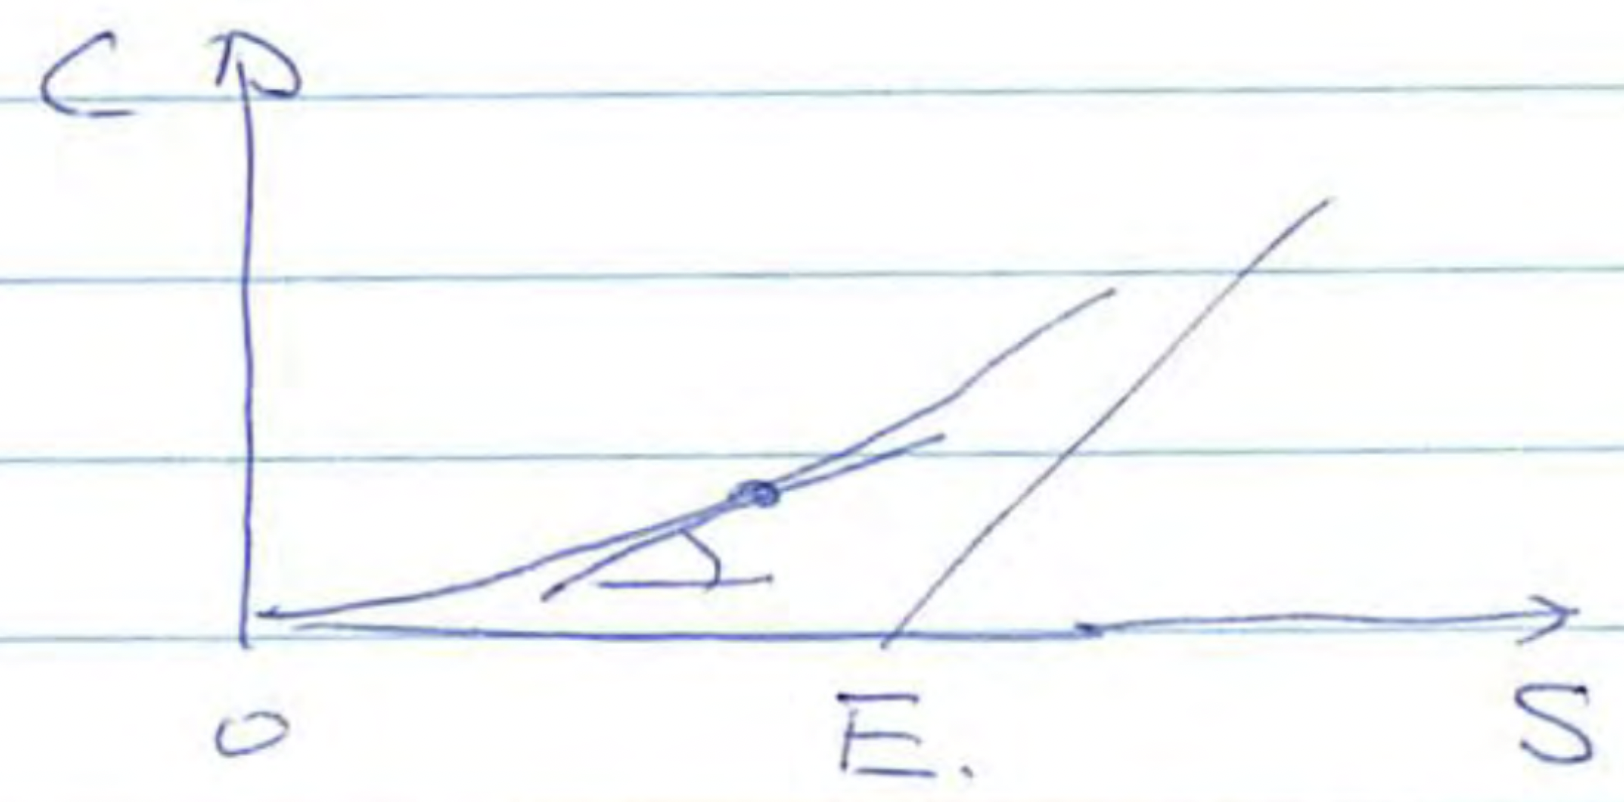
\includegraphics[width=0.7\textwidth]{images/L14-neutralhedge.png}
    \centering
\end{figure}
\end{frame}

\begin{frame}
To derive the PDE for the option we substitute $\alpha_F$ and $\sigma_F$ in the equation relationship:\\
\begin{align*}
    (\alpha-r)\sigma_F &= \sigma(\alpha_F-r)\\
    (\alpha-r)\frac{\sigma\;SF_S}{F} &= \sigma\bigg(\frac{\frac{1}{2}\sigma^2 S^2 F_{SS}+\alpha S F_S - F_\tau}{F}-r\bigg)\\
    \alpha S F_S - r S F_S &= \frac{1}{2} \sigma^2 S^2 F_{SS} + \alpha S F_S - F_\tau -rF...
\end{align*}
\begin{center}
    \boxed{\frac{1}{2}\sigma^2 S^2 F_{SS} + r S F_S - rF - F_\tau = 0}
\end{center}
Fundamental PDE that governs the value of \underline{any} option on S.
\end{frame}

\subsection{Note($\star$)}
\begin{frame}
    
\end{frame}

%%%%%%%%%%%%%%%%%%%%%%%%%%%%%%%%%%%%%%%%%%%%%%%%%%%%%%%%%%%%%%%%%%%%%%%%%%%%%%%%%%%
%%%%%%%%%%%%%% TOPIC 15  The Options Approach to Valuing Risky Debt %%%%%%%%%%%%%%%
%%%%%%%%%%%%%%%%%%%%%%%%%%%%%%%%%%%%%%%%%%%%%%%%%%%%%%%%%%%%%%%%%%%%%%%%%%%%%%%%%%%
\section{The Options Approach to Valuing Risky Debt}
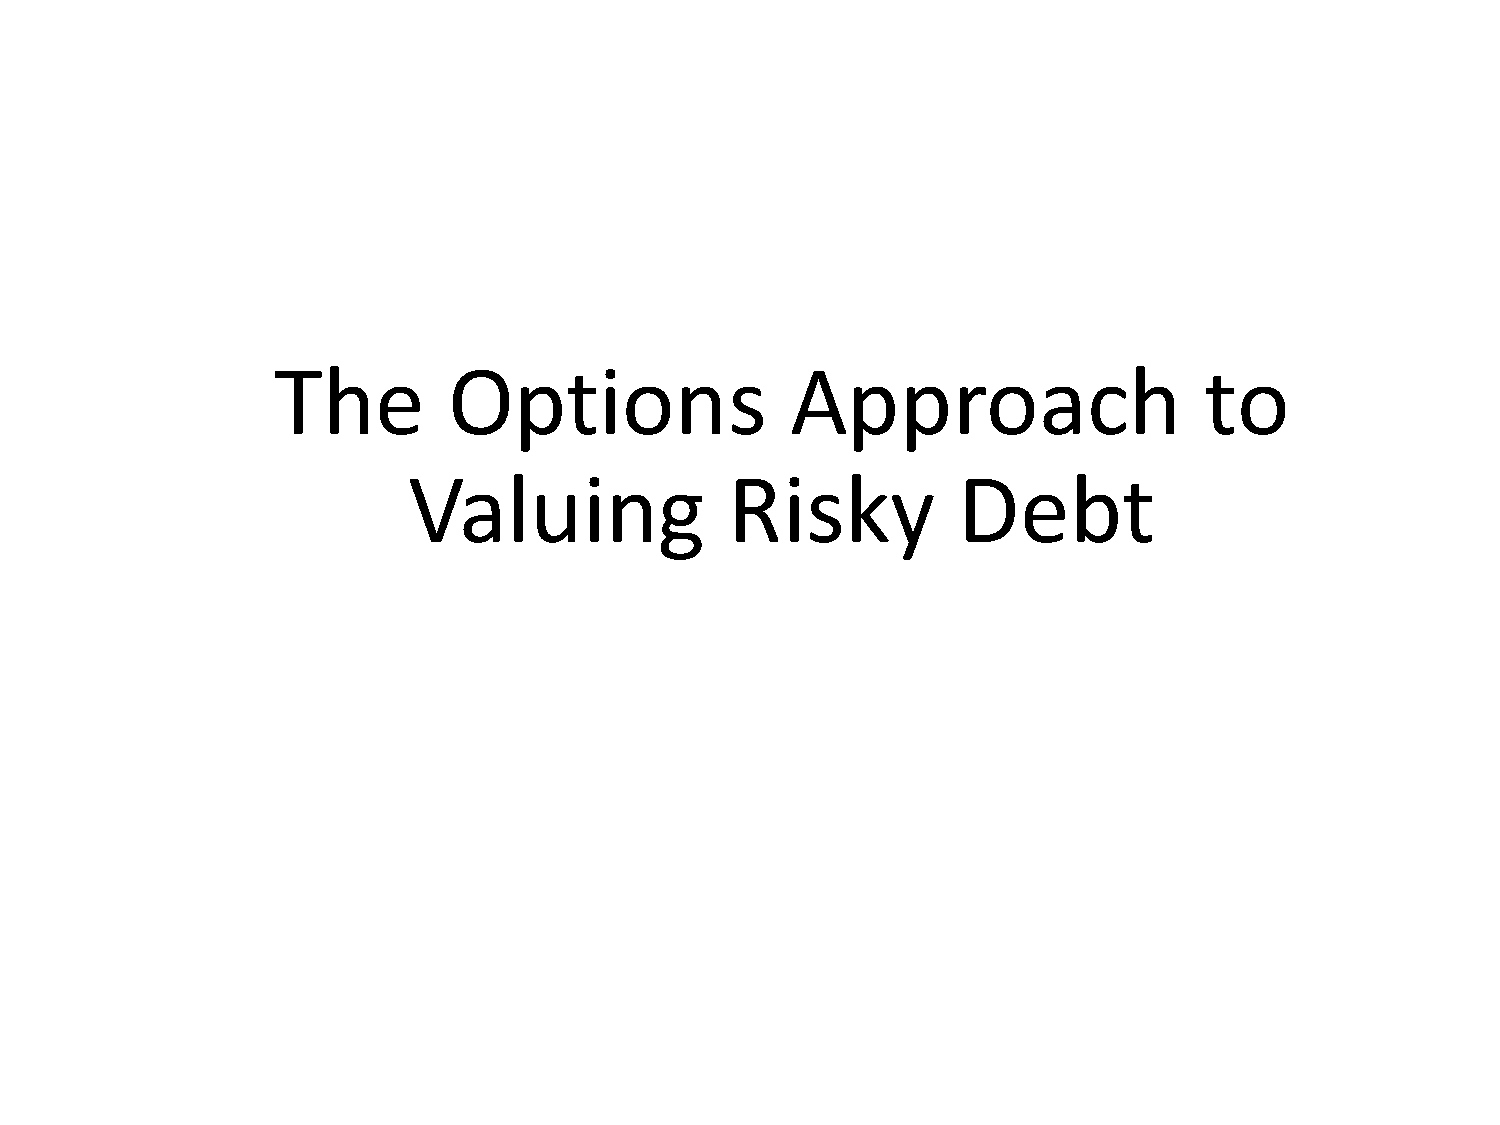
\includepdf[page={2-}]{pdfs/topic15}

%%%%%%%%%%%%%%%%%%%%%%%%%%%%%%%%%%%%%%%%%%%%%%%%%%%%%%%%%%%%%%%%%%%%%%%%%%%
%%%%%%%%%%%%%% TOPIC 16   %%%%%%%%%%%%%%%
%%%%%%%%%%%%%%%%%%%%%%%%%%%%%%%%%%%%%%%%%%%%%%%%%%%%%%%%%%%%%%%%%%%%%%%%%%%
\section{More about Continuous Time Option Pricing}

%%%%%%%%%%%%%%%%%%%%%%%%%%%%%%%%%%%%%%%%%%%%%%%%%%%%%%%%%%%%%%%%%%%%%%%%%%%
%%%%%%%%%%%%%% TOPIC 17   %%%%%%%%%%%%%%%
%%%%%%%%%%%%%%%%%%%%%%%%%%%%%%%%%%%%%%%%%%%%%%%%%%%%%%%%%%%%%%%%%%%%%%%%%%%
\section{Stochastic Models of the Term Structure}

%%%%%%%%%%%%%%%%%%%%%%%%%%%%%%%%%%%%%%%%%%%%%%%%%%%%%%%%%%%%%%%%%%%%%%%%%%%
%%%%%%%%%%%%%% TOPIC 18   %%%%%%%%%%%%%%%
%%%%%%%%%%%%%%%%%%%%%%%%%%%%%%%%%%%%%%%%%%%%%%%%%%%%%%%%%%%%%%%%%%%%%%%%%%%
\section{A Simple Version of CIR}

\section*{References}
\begin{frame}[allowframebreaks]{References}
    \printbibliography
\end{frame}

\end{document}